%% HEADER
%%%%%%%%%%%%%%%%%%%%%%%%%%%%%%%%%%%%%%%%%%%%%%%%%%%%%%%%%%%%%
%%
%%
\newcommand{\hyperrefpdfauthor}{}
\newcommand{\hyperrefpdftitle}{}
\newcommand{\hyperrefpdfsubject}{}
\newcommand{\hyperrefpdfkeywords}{}
\newcommand{\hyperrefpdfborder}{0}
\newcommand{\subfigureautorefname}{\figureautorefname}
\documentclass{styles/wissdoc-kw-eng}

\usepackage{pdfpages}
\usepackage[printonlyused]{acronym}
\usepackage[table]{xcolor}
\usepackage{tikz}
% % newer acronym packaged dont use bflabel anymore,
\providecommand\aclabelfont{} % the new command ist aclabelfont however, we also need to be backwards compatible so... we do it like this
\renewcommand{\aclabelfont}[1]{\normalfont{\normalsize{#1}}\hfill} % keine serifenlose schrift für acronym

% newer acronym packaged dont use bflabel anymore, to not fail the statement below provide the command if not existing
\providecommand\bflabel{} 
\renewcommand{\bflabel}[1]{\aclabelfont{#1}} 

%\usepackage{acronym}
%\usepackage{caption,setspace}
\usepackage{subcaption}
\usepackage[export]{adjustbox}
\usepackage{float}
\floatstyle{ruled}
\newfloat{listing}{htbp}{lop}[chapter]
\floatname{listing}{Listing}
%\usepackage[hang,center,nooneline]{caption}
\captionsetup{font={small,stretch=0.80}}
\captionsetup[subfigure]{justification=centering,labelformat=empty}
\captionsetup[table]{font={small,sf}}
\captionsetup[listing]{font={small,sf}}
\usepackage[absolute]{textpos}
\usepackage{styles/etoolbox}
%% Normales LaTeX oder pdfLaTeX? %%%%%%%%%%%%%%%%%%%%%%%%%%%%
%% ==> Das neue if-Kommando "\ifpdf" wird an einigen wenigen
%% ==> Stellen benötigt, um die Kompatibilität zwischen
%% ==> LaTeX und pdfLaTeX herzustellen.
%\newif\ifpdf
%\ifx\pdfoutput\undefined
%    \pdffalse              %%normales LaTeX wird ausgeführt
%\else
%    \pdfoutput=1
%    \pdftrue               %%pdfLaTeX wird ausgeführt
%\fi


%% Fonts für pdfLaTeX %%%%%%%%%%%%%%%%%%%%%%%%%%%%%%%%%%%%%%%
%% ==> Nur notwendig, falls keine cm-super-Fonts installiert
\ifpdf
	\usepackage{ae}       %%Benutzen Sie nur eines dieser Pakete:
	%\usepackage{zefonts}  %%je nachdem, welches Sie besitzen.
\else
	%%Normales LaTeX - keine speziellen Fontpackages notwendig
\fi

%% zur Zitaten des Quelltextes%%%%%%%%%%%%%%%%%%%%%%%%%%%%%%%
% "final" forces printing of all listings, even if the global "draft" is set
\usepackage[final]{listings}
\lstset{
    basicstyle=\footnotesize\ttfamily,
    tabsize=4,
    numberstyle=\tiny\color{gray},
    numbersep=5pt,
    numbers=left,
    captionpos=b,
    abovecaptionskip=0pt,
    belowcaptionskip=0pt,
    aboveskip=10pt,
    belowskip=0pt,
    floatplacement=tbp,
    frame=topline,
    framerule=.1pt,
    framesep = 3pt,
    }
\renewcommand\lstlistingname{\textbf{Listing}}
% This is only kept for backwards compatibility. You should never have to use it. Use the listing-environment instead.
%\DeclareCaptionFormat*{lstruled}{{\bfseries#1\small\space\normalfont#3\hrule height.1pt depth0pt}\par}
%\captionsetup[lstlisting]{format=lstruled,singlelinecheck=false}

%% mehrere Abbildungen in eine %%%%%%%%%%%%%%%%%%%%%%%%%%%%%%


%% Packages für Formeln %%%%%%%%%%%%%%%%%%%%%%%%%%%%%%%%%%%%%
\usepackage{amsmath}
\usepackage{amsthm,amssymb}
\usepackage{amsfonts}


%% Zeilenabstand %%%%%%%%%%%%%%%%%%%%%%%%%%%%%%%%%%%%%%%%%%%%
\usepackage{setspace}
%\singlespacing        %% 1-zeilig (Standard)
%\onehalfspacing       %% 1,5-zeilig
%\doublespacing        %% 2-zeilig


%% Andere Packages %%%%%%%%%%%%%%%%%%%%%%%%%%%%%%%%%%%%%%%%%%
%\usepackage{a4wide} %%Kleinere Seitenränder = mehr Text pro Zeile.
\usepackage{fancyhdr} %%Fancy Kopf- und Fußzeilen
%\usepackage{longtable} %%Für Tabellen, die eine Seite überschreiten
\usepackage{lscape}
\usepackage{rotating} 
%\usepackage[htt]{hyphenat} %Trennung von Typewriter-Schriften
%\usepackage{listings}


% Tabellen mit Center und left
\usepackage{tabularx,colortbl} % colored table background
\newcolumntype{C}[1]{>{\centering\arraybackslash}p{#1}}
\newcolumntype{R}[1]{>{\raggedleft\arraybackslash}p{#1}}
% Table spacings
\newcommand\T{\rule{0pt}{2.5ex}\rule[-1.0ex]{0pt}{0pt}}
\newcommand\B{\rule[-1.0ex]{0pt}{0pt}}

\definecolor{slightgray}{gray}{.90} 


%% Definitionen %%%%%%%%%%%%%%%%%%%%%%%%%%%%
\newcommand{\todo}[1]{ \textcolor{red}{\textbf{TODO: #1}} }

%% zur Benutzung bei ergänzenden Daten%%%%%%%%%%%%%%%%%%%%%%%%
%\usepackage{endnotes}
%\renewcommand{\notesname}{Konfigurationsdaten der Messreihen}
%\renewcommand{\theendnote}{\Alph{endnote}}
%\renewcommand{\enotesize}{\normalsize}

%\hyphenation{Sensor-netz-werk
%}

%%%%%%%%%%%%%%%%%%%%%%%%%%%%%%%%%%%%%%%%%%%%%%%%%%%%%%%%%%%%%
%% DOKUMENT
%%%%%%%%%%%%%%%%%%%%%%%%%%%%%%%%%%%%%%%%%%%%%%%%%%%%%%%%%%%%%
\begin{document}

%% Dateiendungen für Grafiken %%%%%%%%%%%%%%%%%%%%%%%%%%%%%%%
%% ==> Sie können hiermit die Dateiendung einer Grafik weglassen.
%% ==> Aus "\includegraphics{titel.eps}" wird "\includegraphics{titel}".
%% ==> Wenn Sie nunmehr 2 inhaltsgleiche Grafiken "titel.eps" und
%% ==> "titel.pdf" erstellen, wird jeweils nur die Grafik eingebunden,
%% ==> die von ihrem Compiler verarbeitet werden kann.
%% ==> pdfLaTeX benutzt "titel.pdf". LaTeX benutzt "titel.eps".
%\ifpdf
%    \DeclareGraphicsExtensions{.pdf,.jpg,.png}
%\else
%    \DeclareGraphicsExtensions{.eps}
%\fi

\pagestyle{empty} %%Keine Kopf-/Fusszeilen auf den ersten Seiten.

\ifnotdraft{
%% Deckblatt %%%%%%%%%%%%%%%%%%%%%%%%%%%%%%%%%%%%%%%%%%%%%%%%
\frontmatter
% !TEX root =  ../thesis.tex

\titlehead{
%	\hfill
%	
\includegraphics[width=10cm,keepaspectratio]{logos/rwth}
} % end titlehead


\begin{titlepage}

\begin{textblock*}{10cm} (12.7cm,2.7cm)

\includegraphics[width=10cm,keepaspectratio]{logos/rwth}
\end{textblock*}

\let\footnotesize\small \let\footnoterule\relax

\hbox{}
\vfill

\centering

\begin{doublespace} 
{ \huge\sffamily\textbf{An EMG-based Method for}}\\ \vspace{0.7em}
 {\huge\sffamily\textbf{Finger Gesture Recognition}} \\ \vspace{0.2em}

\end{doublespace}
\vskip 2cm

{\large\sffamily

Master Thesis\\[5pt]
\textbf{Ioannis Agalliadis}
\vskip 1cm

This work was submitted to the\\[5pt]
\textbf{Department of Medical Informatics\\[5pt]
        RWTH Aachen University, Germany}
\vskip 2cm

Adviser(s):
\vskip 2mm
Dr. Stephan Jonas\\
Marko Jovanovi{\' c}
\vskip 5mm
Examiners:
\vskip 2mm
Univ.-Prof. Dr.med. Dr.rer.nat. Dipl.-Math. Klaus Kabino\\
Prof. Dr. Jan Borchers
\vskip 1cm

\begin{tabular}{R{6cm}p{6cm}}
Registration date:  & 2017-12-13 \\
Submission date:    & 2017-04-10 \\
\end{tabular}

} %\large\sffamily

\vfill

\end{titlepage}

\cleardoublepage

\cleardoublepage
% !TEX root =  ../thesis.tex
\includepdf[pages={1},offset=75 -75,pagecommand={
\begin{tikzpicture}[remember picture,overlay,shift={(current page.center)}]
\coordinate (begin-generic) at (5.3,11.3);
\coordinate (end-generic) at (6.4,11.3);
\coordinate (begin-bachelor) at (6.45,11.3);
\coordinate (end-bachelor) at (9,11.3);
\coordinate (begin-master) at (-5.4,10.8);
\coordinate (end-master) at    (-3.15,10.8);
\node at (-5.5,13.4)
       [text width=7cm,rounded corners,below right]
{
Agalliadis, Ioannis
};
\node at (3.25,13.4)  [text width=5cm,rounded corners,below right]
{
359894 % This is optional
};
% ===== for type generic uncomment the next 2 lines =====
% \draw[line width=1mm] (begin-bachelor) -- (end-bachelor);
% \draw[line width=1mm] (begin-master) -- (end-master);
% ===== for type bachelor uncomment the next 2 lines =====
%\draw[line width=1mm] (begin-generic) -- (end-generic);
%\draw[line width=1mm] (begin-master) -- (end-master);
% ===== for type master uncomment the next 2 lines =====
 \draw[line width=1mm] (begin-generic) -- (end-generic);
 \draw[line width=1mm] (begin-bachelor) -- (end-bachelor);
%
\node at (-5.5,10.4)
       [text width=16.5cm,rounded corners,below right]
{
An EMG-based Method for Finger Gesture Recognition
};
\node at (-5.5,4.6)
       [text width=7cm,rounded corners,below right]
{
Aachen, 10.04.2018
};
\node at (-5.5,-8.45)
       [text width=7cm,rounded corners,below right]
{
Aachen, 10.04.2018
};
\end{tikzpicture}
}]{Formular_Eidesstattliche_Versicherung_neu.pdf}

\cleardoublepage
\cleardoublepage
\vspace {2cm}
\begin{center}
\paragraph{Abstract}
\hrulefill
\end{center}
Wearable devices have been evolving over the last years. The integration of sensors on them encourages scientists to use wearable devices more frequently as they are cheaper and the purchasing accessibility is easier than other specialized devices. In this work, we will use a gesture control armband called Myo. Myo is equipped with a gyroscope, magnetometer, accelerometer and a set of electromyographic (EMG) sensors. Along with the Myo we will use a cell phone which receives the signals from the Myo. The focus point of this master thesis is to research different features based only on EMG signals coming from finger movements. EMG is a signal measurement of the electrical activity of the muscles and is one of the most common sources of information used to study muscle function and neurological disorders. One of the main reasons behind that is that we want to correctly detect finger movements using only the EMG signals that are associated only with arm muscles responsible for motoring the fingers. Also, the existing literature is limited on finger gesture recognition using non-intruding device such as Myo \cite{myo}. The goal of this master thesis is to apply the earned knowledge to Myo controlled prosthetic arms worn by amputees that have lost some or all of their fingers or patients that have deficiency of moving their fingers due to a stroke, tendinitis, or peripheral neuropathy. The fact that each finger has a different degree of freedom (DoF) gives us the chance to detect various finger gestures. The most trite ones which we will examine are the extension and the flexion of a finger or a group of fingers. In particular, the thumb can be flexed and extended (2 DoF). The rest of the fingers can be flexed and extended in one direction (1 DoF). The need of a solid classification between these two different kind of movements is imperative. What’s more, there can be more combinations such as holding three fingers (thumb excluded) as a cluster and moving forward backward the remaining free finger. The increasing degree of complexity of the different finger gestures plays a significant role in order to have a more complete detection cover over the whole spectrum of finger gestures. After the collection of the recordings, we will introduce a preprocessing stage which will help us in extracting features from the raw data. In this work, we will use a range of methods such as root mean square (RMS), moving average (smooth), Short-Time Fourier Transform (STFT) and a variety of discrete wavelet transforms. The collection of all feature extraction vectors will then be passed into classifiers and classification errors from each feature will be compared with each other in order to determine the best performance. In the implemented framework we will examine the approach of an \ac{ANN} classifier.

\cleardoublepage
\cleardoublepage

\chapter*{Acknowledgments}

I want to thank my advisers Marko Jovanovi{\' c} and Dr. Stephan Jonas for their scientific assistance and continuous support over this period. Special thanks to Dr. Ekaterina Kutafina for providing me also ideas for my master thesis.
I would like to thank also the mHealth group generally for creating a friendly and supportive environment.\\
Furthermore, I want to thank my family for motivating me to finish my master thesis.\\
Finally, I want to thank Univ.-Prof. Dr.med. Dr.rer.nat. Dipl-Math Klaus Kabino and Prof. Jan Borchers for the possibility to write this thesis as well as supervising it.
\cleardoublepage

% Titelseite hatte noch normale Tabellen. Von hier ab sollen alle
% Tabellen laut style-Vorgaben sans serif sein.
\AtBeginEnvironment{tabular}{\sffamily}
\AtBeginEnvironment{tabularx}{\sffamily}

%% Inhaltsverzeichnis %%%%%%%%%%%%%%%%%%%%%%%%%%%%%%%%%%%%%%%
\tableofcontents %Inhaltsverzeichnis
\cleardoublepage %Das erste Kapitel soll auf einer ungeraden Seite beginnen.
} % end ifnotdraft

\pagestyle{fancy} %%Ab hier die Kopf-/Fusszeilen: headings / fancy / ...

%%%%%%%%%%%%%%%%%%%%%%%%%%%%%%%%%%%%%%%%%%%%%%%%%%%%%%%%%%%%%
% einzelne Kapitel
%%%%%%%%%%%%%%%%%%%%%%%%%%%%%%%%%%%%%%%%%%%%%%%%%%%%%%%%%%%%%
%\input{commands}

\mainmatter
\input{chapters/01_Introduction}
\chapter{Methods}
The proposed processing techniques and methods used for evaluating finger movements and recognizing errors requires six steps:  (1) removal of artifacts from \ac{EMG} data, (2) segmentation of the \ac{EMG} data into individual movements, (3) division of the \ac{EMG} data into 11 folds (11 is the number of the features we are preprocessing the EMG data with), (4) windowing, (5) feature extraction, (6) classification. The machine learning model learns the patterns of the preprocessed data by the selected features, segmented individual finger movements. Based on the detection accuracies of each machine learning model, allows us to have feedback on which of the features are working best on the \ac{EMG} data.\\
\section{Pipeline summary}
In Fig. \ref{fig:pipeline_summary} the overview of the system's pipeline is depicted. \\
\begin{figure}[h!]
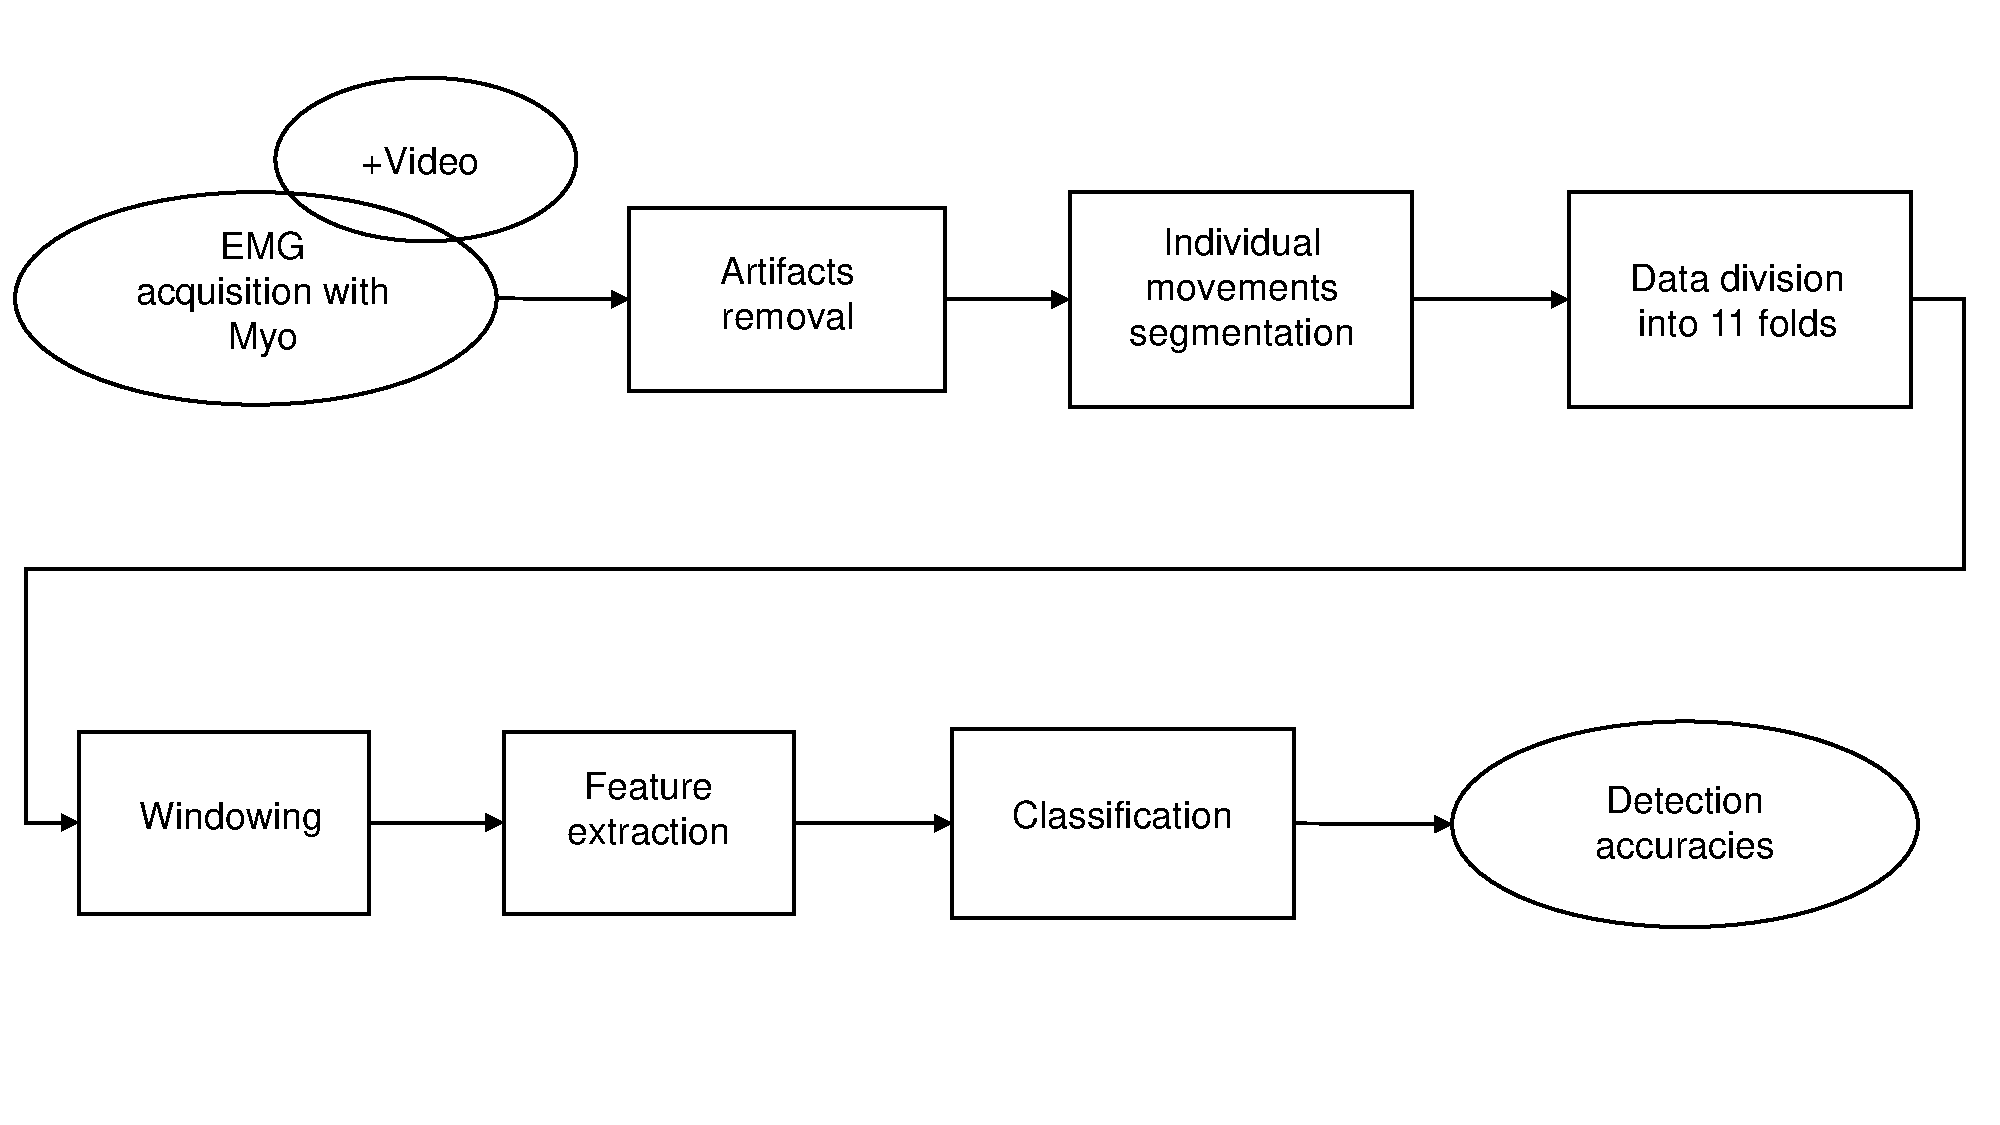
\includegraphics[width=15cm,left,keepaspectratio]{figures/pipeline_summary.pdf}
\caption{Overview of the pipeline}
\label{fig:pipeline_summary}
\end{figure}
\section{Data collection}
In Fig. \ref{fig:data_collection} we can see how the data are acquired. Firstly, the subject wears the Myo armband in his/her arm and via Bluetooth connection the Myo armband is connected with a mobile phone. After the completion of the corresponding finger gesture the zip folder with the acquired signals and the video recording are uploaded to the cloud. The \ac{EMG} signals and the video recordings are downloaded to the PC. The video recording is used next, in order to determine the intervals of the gestures we are interested in. Then, we input the frames of interest in the Cutter App, an application implemented by Seiffarth Johannes, and the \ac{EMG} signals are segmented in the corresponding frame intervals. Also, with the same application we can visualize the \ac{EMG} waveforms of the different recordings and to remove any artifacts. In the current work, due to the variable frame rate of the cell phone's camera the frames of the video did not correspond to the corresponding waveform in time, thus leading to artifacts. This behavior of the mobile device's camera happened unexpectedly during the different takes. Therefore, every recording was examined carefully before segmenting it.
\begin{figure}[h!]
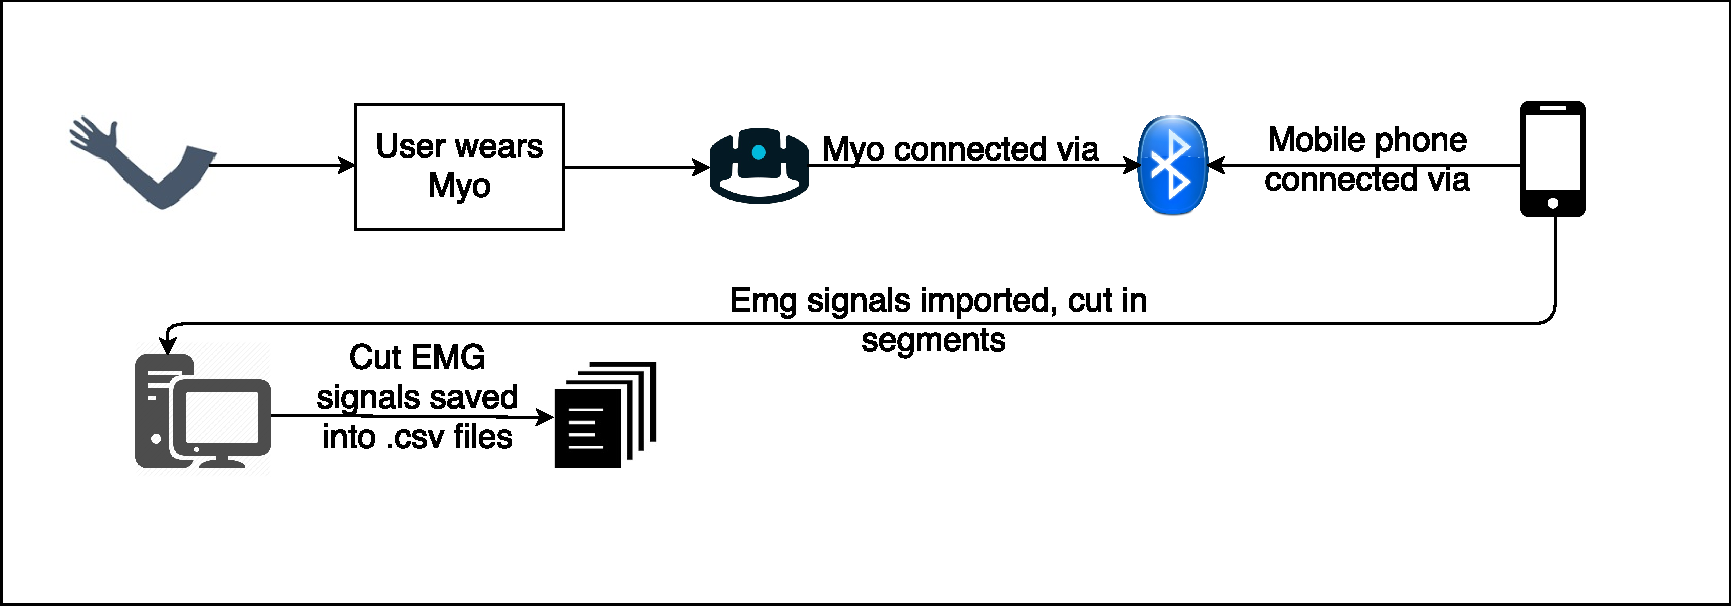
\includegraphics[width=15cm,left,keepaspectratio]{figures/data_collection}
\caption{Data collection}
\label{fig:data_collection}
\end{figure}
\section{Cross-Validation}
Next, as the Fig. \ref{fig:division_into_5_folds} demonstrates, the data are divided into training, testing and evaluation folders. Specifically, we start by removing 20\% of the segmented data and we create a evaluation folder with this data. Until the machine learning model is fully developed we do not touch the data from the evaluation folder. In addition, cross validation technique allows to compensate for small data sets and makes our results more robust. Then, we have to decide on the number of the folds. If we choose a large number of folds we will have too little data in each fold and if we choose a small number of folds, the method will not be serving its purpose. In our case, we choose to create five training and test folds and one evaluation folder. The remaining 80\% of the data, will be our train and test data.\\
After the creation of the evaluation folder, we create the five test folders by dividing randomly the remaining data accordingly to the number of the folders we created. In our case, we take a random 20\% from the remaining data and distribute it to each of the five test folders. Then, we create each of the five train folders by combining all the data from the test folders but excluding the folder with the mutual shared number. For example, the train folder with the number one will take all the data from the test folders with the number two, three, four and five thus, excluding the test folder with the number one. This applies for the rest of the train folders. After the completion of all of the above steps, we end up having five folders with train and test data and one evaluation folder storing our segmented EMG signals and ready to input them to our machine learning models.
\begin{figure}[h!]
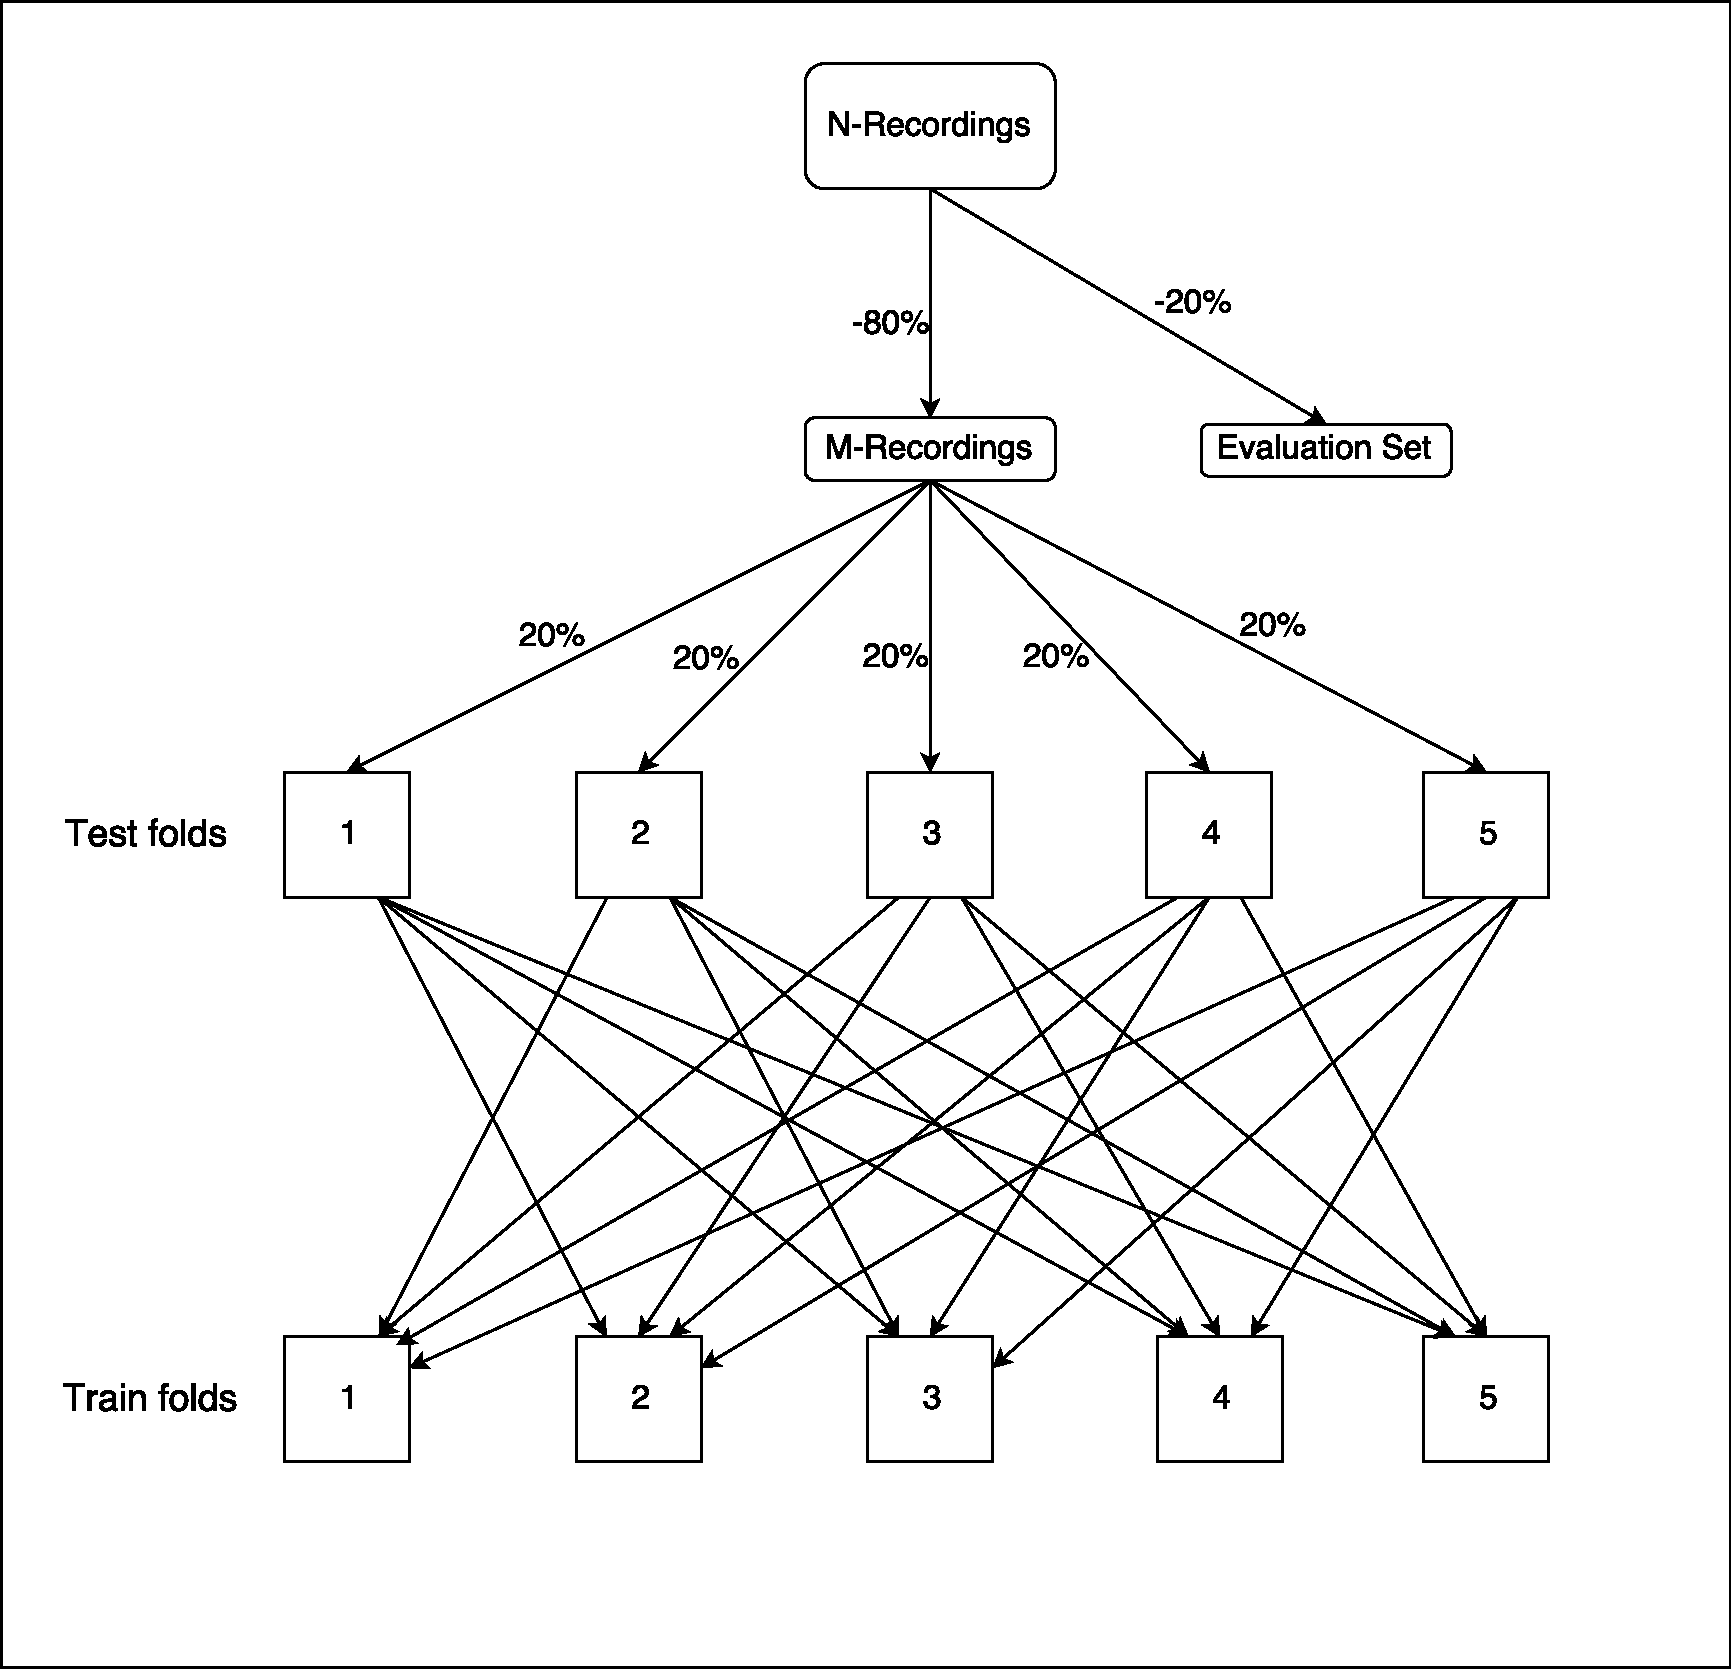
\includegraphics[width=15cm,left,keepaspectratio]{figures/data_division}
\caption{Division of recording into 5 folds}
\label{fig:division_into_5_folds}
\end{figure}

\section{Windowing}
Windowing is a common technique in machine learning to improve the detection accuracies. It is a procedure that is applied to the training and testing data before they are fed into the machine learning and thus it can be universally applied, independently of the  classification algorithm  in use  \cite{dietterich_machine_2002}. \\
In order to forward the data into the machine learning algorithm we often have to apply windowing to the data in order to properly format them as an input. In our experiments we acquire raw EMG data from the Myo that are captured at a fixed sampling frequency of 200 Hz. We force the classifier to take a certain perspective on the problem by defining a sample to consist of this set. 
Windowing is a way to avoid the problem of comparatively long ranges of samples by reducing the input vector's length. We define a window length \textit{w} and reshape the input vector in such a way that each input vector contains \textit{w} sensor readings. For example, if we acquire the EMG data of one Myo armband and assume a window of size \textit{w} = 10, each input vector contains not just 8, but 80 values, corresponding to 10 consecutive readings of the 8 EMG sensors in one Myo armband.\\
With this technique, each output value corresponds to larger set of sensor readings, more actual muscle activity is mapped to a gesture. This seems to be reasonable approach when looking at the vast differences in resolution: up to 200 sensor readings per second vs. one gesture change every few seconds. In such a manner, this approach forces the classifier to look at the data through a window that shows a more expressive excerpt of the input data.\\
The disadvantage that comes with windowing is that every value \textit{w} that is used creates an artificial connection between those \textit{w} values of input data that either may or may not be relevant to determine the corresponding output values. For example, if the window length \textit{w} is wide, a window can contain data that belongs to multiple gestures. On the contrary, if the window is narrow it may not contain the necessary number of samples to characterize succesfully the multiple gestures. That is why \textit{w} needs to be chosen carefully.\\
A solution to overcome this particular problem of windowing is to create \textit{overlapping} windows. Without overlapping windows each sample is somehow treated with the same weight. However, when someone observes the extracted features from two consecutive frames the change of property between the frames may induce a discontinuity. With the overlapping though, some $x_i$ of the original input vector will land in multiple windows. With this way, each measurement can be viewed twice but in a different context.\\
Depending on the value \textit{o} which is bounded with $0 \leq o \leq w-1$ this can increase  the size of the input vector. At the cost of larger vector sizes and effectively more computation time, overlapping windows  can reduce the impact of the artificial connection between values that is introduced by windowing. \\
\subsection{Windowing in current work}
In our case, Fig. \ref{fig:windowing} states that we take each train, test and evaluation sets and we apply a window of 128 length with a step of one to each recording. For the sake of computation time we changed the step from one to 64 for the later experiments. Each row of each recording consists of nine columns where the first column is the timestamp and the rest eight columns are the indicators from the eight \ac{EMG} sensors. All the produced 128-length windows are concatenated vertically in a final array.
\begin{figure}[h!]
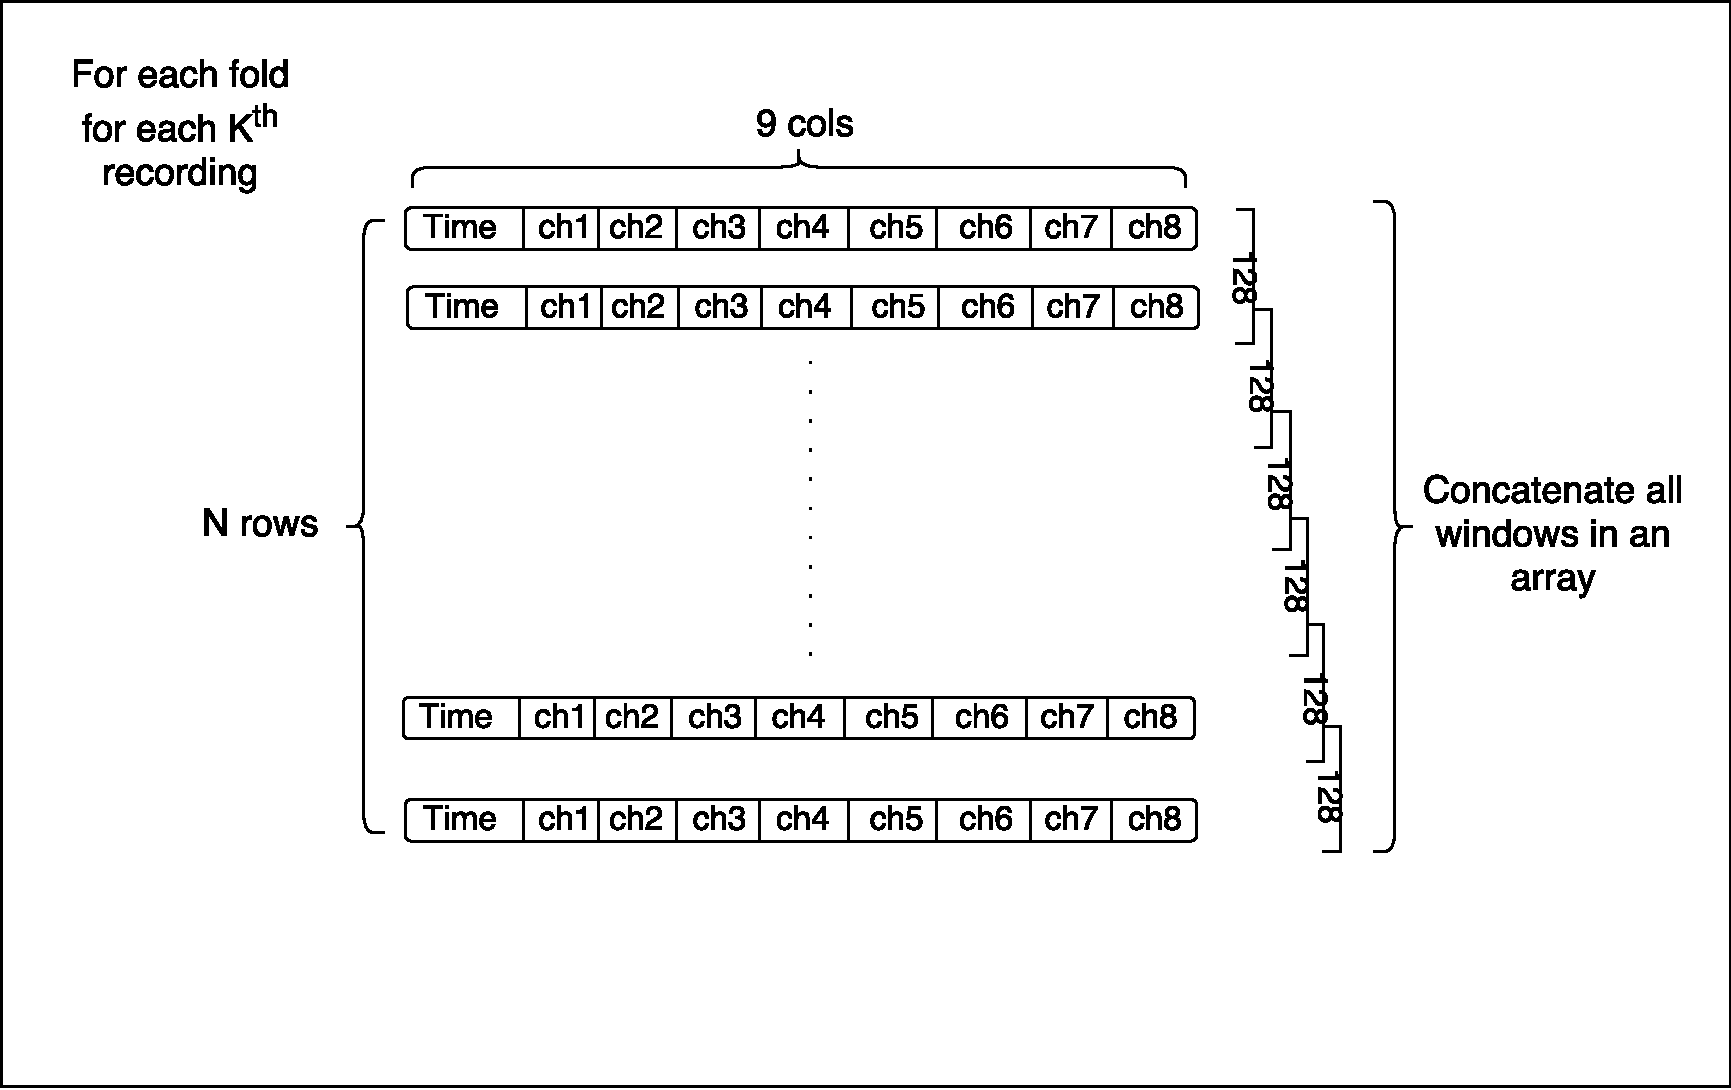
\includegraphics[width=15cm,left,keepaspectratio]{figures/windowing}
\caption{Windowing}
\label{fig:windowing}
\end{figure}

\section{Feature extraction}
The information extracted from the \ac{EMG} signals, which are represented in a feature vector, is chosen to help in minimizing the classification error which show us which of the selected features have the possibility for the most efficient identification of the each finger gesture. \\

In this section we are going to explain further the methods we used to extract the features from the acquired EMG signals. 
\subsection{Moving average}
The moving average function, calculates a series of averages from successive segments of a series of values. A moving average is used with time series data to smooth out short-term fluctuations as our data are already noisy. The simple moving average is taken from an equal number of data points on either side of a central value. This requires using an odd number of values in the sample window. In our case, moving average is taken in a window size of five. The definition of the arithmetic mean is given by the following equation \cite{whittaker_calculus_1924}:
\begin{equation}
s_i = \frac{1}{n} \sum_{j=1}^{i+n-1}\alpha_j
\end{equation}
\subsection{Root mean square}
Root mean square (abbreviated RMS and sometimes called the quadratic mean) is the square root of the arithmetic mean of the squares of a set of values. The equation is following:
\begin{equation}
x_{RMS} = \sqrt{\frac{x_1^2+x_2^2+ \hdots + x_n^2}{n}} =
          \sqrt{\frac{\sum_{i=1}^{n}x_i^2}{n}} = \sqrt{\langle x^2 \rangle}
\end{equation}
where $\langle x^2 \rangle$ is the arithmetic mean of the series $x_i^2$ \cite{kenney_mathematics_2013}. If $x$ is a row or a column vector, $x_{RMS}$ is a real-valued scalar. 
\subsection{Short-time Fourier transform}
STFT is a well known technique in signal processing to analyze non-stationary signals. Particularly, STFT helps to analyze a small section of the signal over time thanks to the \textit{windowing} function applied (e.g., Hann, Gaussian) on the signal. Fig. \ref{fig:fft} shows us in brief how STFT works.
\begin{figure}[!htb]
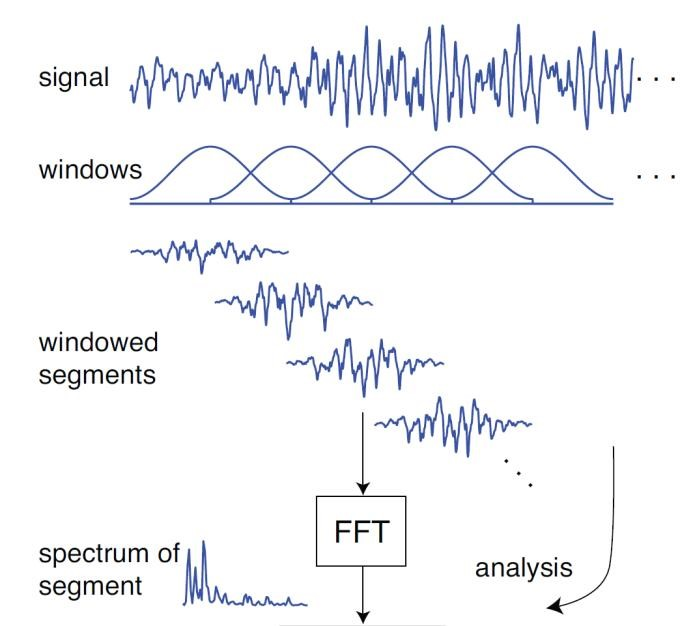
\includegraphics[width=10cm,center,keepaspectratio]{figures/fft}
\caption{Application of the STFT in the segmented windows \cite{sethares_rhythm_2007}}
\label{fig:fft}
\end{figure}
STFT maps a signal into a two-dimensional function of time and frequency. Each section, that means $x[n]w[n-m]$ is Fourier transformed, and the complex result is added to a matrix, which records magnitude and phase for each point in time and frequency. This can be expressed as:
\begin{equation}
\textbf{STFT}{x[n]}(m, \omega) \equiv X(m, \omega) = \sum_{n = - \infty}^{\infty}x[n]w[n-m]\exp^{-j\omega n}
\end{equation}
with signal $x[n]$ and window $w[n]$. STFT provides information about when and which frequencies in a signal occurs. One can obtain that information with a limited precision depending on the size of the window.  As the size of the time window is the same for all frequencies this constitutes a disadvantage and leads to cutting valuable information. To determine accurately time or frequency one need to vary the window size. The weak point of STFT is that whoever wants to use it will face the problem of resolution. Which means that there is a question of what window size should someone choose. Narrow windows offer good time resolution but poor frequency resolution. Wide windows offer good frequency resolution but poor time resolution \cite{polikar_wavelet_1996}. To visualize what we explained with words, in Fig. \ref{fig:spectrograms} we produce four spectrograms to emphasize between the different effect the window size of STFT has on the signal that is consisted from simple stationary sinusoidal waveforms joined together. The signal is sampled at frequency 400 Hz:
\begin{equation}
x(t) = \begin{cases}
      cos(2 \pi 10 t) & 0s \leq t < 5s \\
      cos(2 \pi 25 t) & 5s \leq t < 10s\\
      cos(2 \pi 50 t) & 10s \leq t < 15s \\
      cos(2 \pi 100 t) & 15s \leq t < 20s
\end{cases}
\end{equation}
\begin{figure}[!htb]
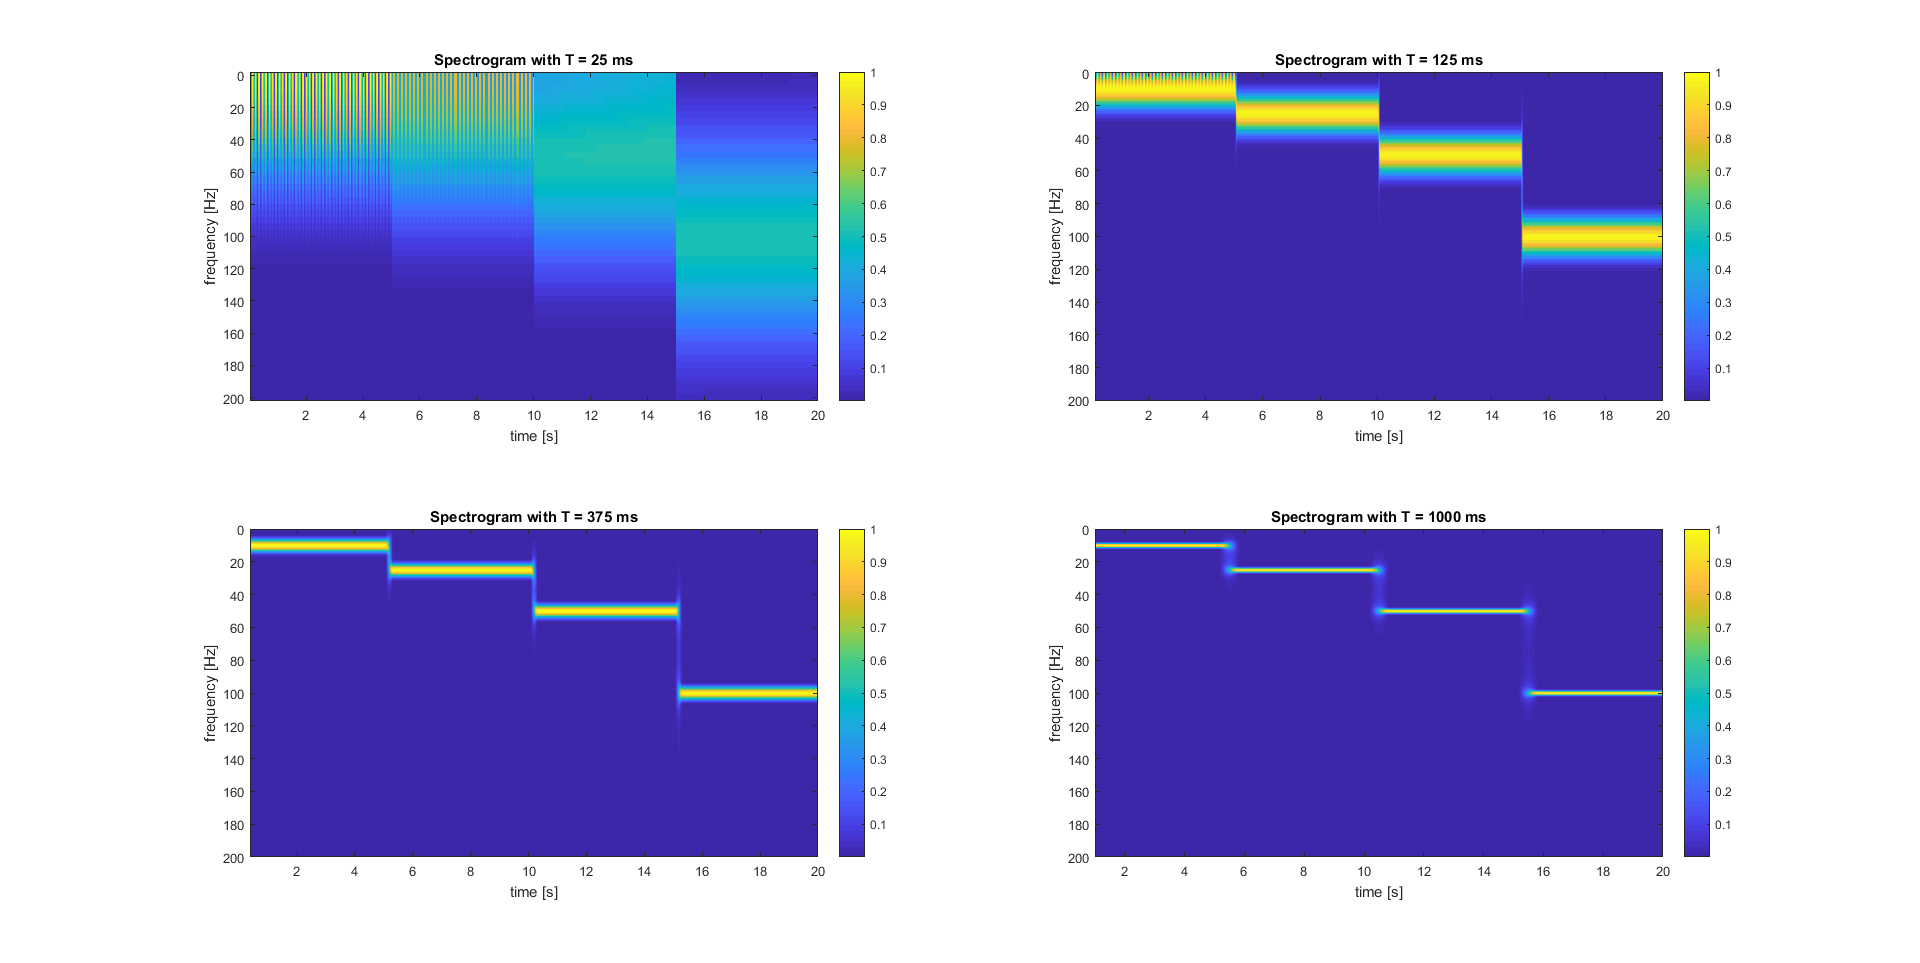
\includegraphics[width=20cm,center,keepaspectratio]{figures/spectrograms}
\caption{Spectrograms of the thumb extension}
\label{fig:spectrograms}
\end{figure}
As we can observe, with the 25 ms window we are able to say with great precision when the frequency of the signal changes but to identify which frequencies exist in the signal still remains a difficult task. On the contraty, with bigger window sizes such as with T = 1000 ms we can detect with great precision which frequencies exist in the signal while the determination of the periods when these frequencies happen is difficult to distinguish because of the blur.
\newpage
The spectrogram we used to visualize the STFT of the signals is generated by the squared magnitude of the STFT. The equation is following:
\begin{equation}
\textbf{spectrogram}\{x(t)\}(\tau, \omega) \equiv \left|X(\tau, \omega)\right|^2
\end{equation}
In the Fig. \ref{fig:STFT_ch7_ext} we can see the spectrogram of a signal coming from the thumb extension and in the Fig. \ref{fig:STFT_ch7_flx} we can see the spectrogram of a signal coming from the thumb flexion.
\begin{figure}[!htb]
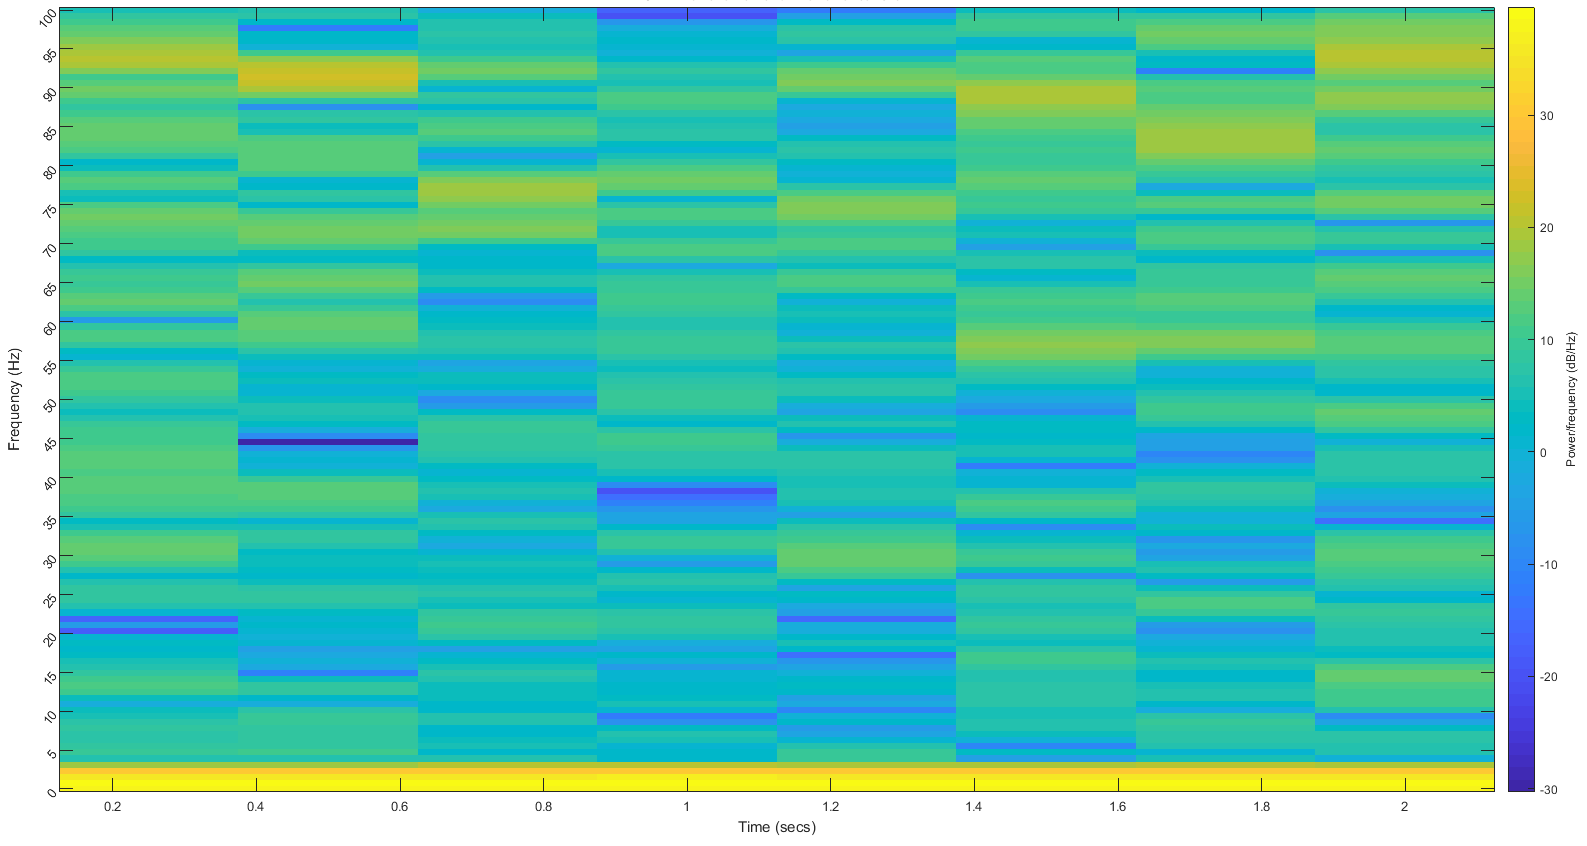
\includegraphics[width=16cm,left,keepaspectratio]{figures/STFT_ch7_ext}
\caption{Spectrogram of the thumb extension from Myo's 7th channel}
\label{fig:STFT_ch7_ext}
\end{figure}
\begin{figure}[!htb]
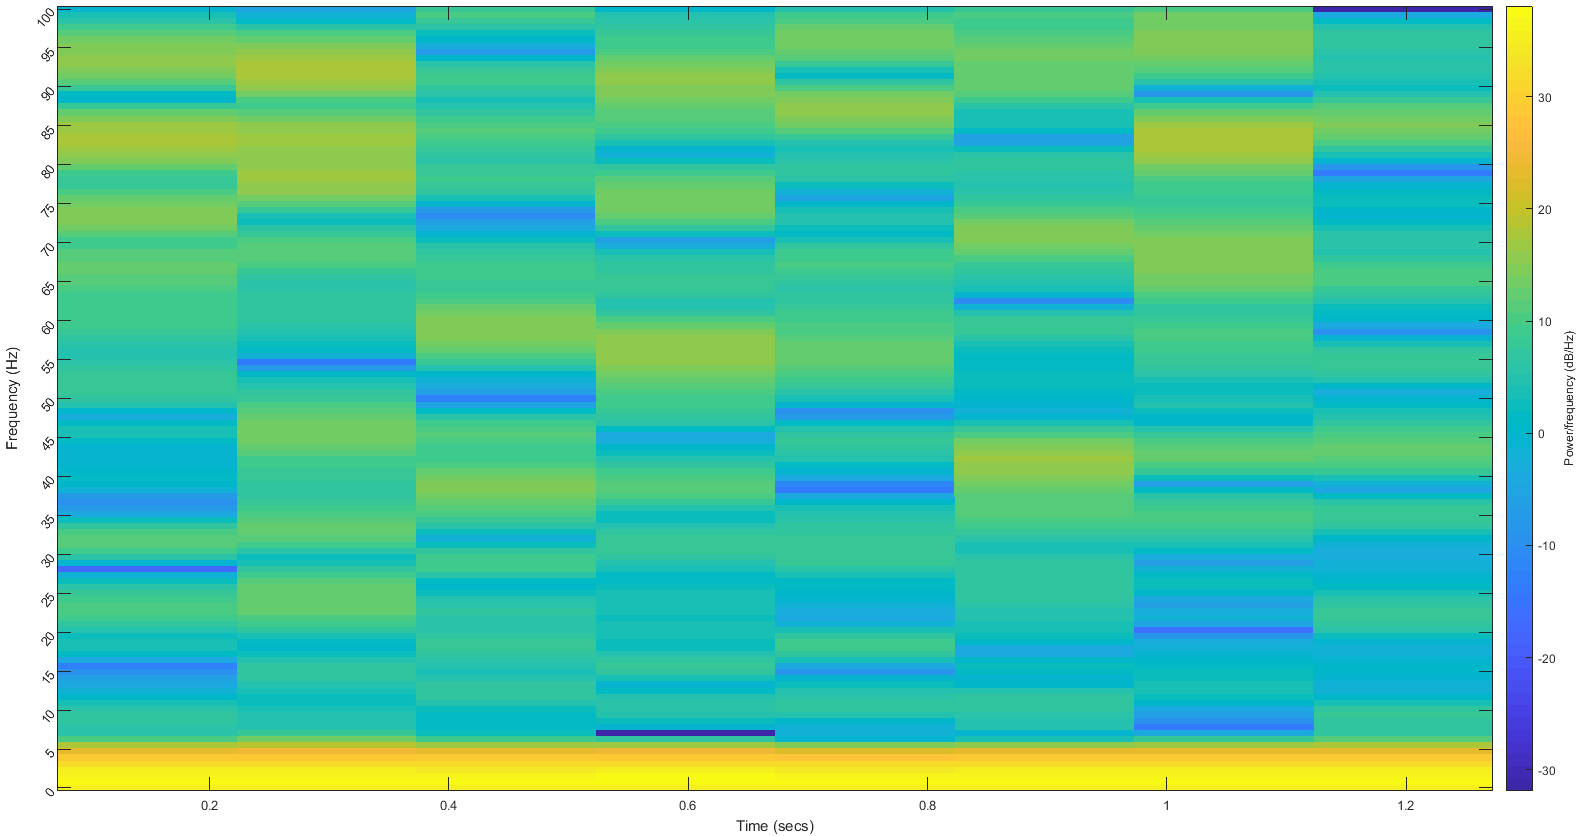
\includegraphics[width=16cm,left,keepaspectratio]{figures/STFT_ch7_flx}
\caption{Spectrogram of the thumb flexion from Myo's 7th channel}
\label{fig:STFT_ch7_flx}
\end{figure}
The spectrogram can be represented as a visual heat map where the horizontal axis represents the time axis and the vertical axis represents the frequency axis. In the above image the darker colors visualize for a particular time point and a particular frequency low magnitude. So, the darker the colors the lower the magnitude and similarly the higher in magnitude the frequency component is, the lighter the color.
\subsection{Wavelet Analysis}
Wavelet analysis (also called wavelet theory or just wavelets) has attracted much attention in signal processing. In order to overcome the resolution problem with the fixed window size in Fourier Transform a different approach is employed. Like Fourier analysis, wavelet analysis deals with expansion of functions in terms of a set of basis functions. Unlike Fourier analysis, wavelet analysis expands functions not in terms of trigonometric polynomials but in terms of wavelets, which are generated in the form of translations and dilations of a fixed function called the mother wavelet \cite{lee_wavelet_1994}. \\
A wavelet is a little wave oscillation with an amplitude that begins at zero increases and decreases back to zero. The original signal is convoluted with the wavelets. With this way, useful information is extracted from the raw signals. \\
\begin{figure}[H]
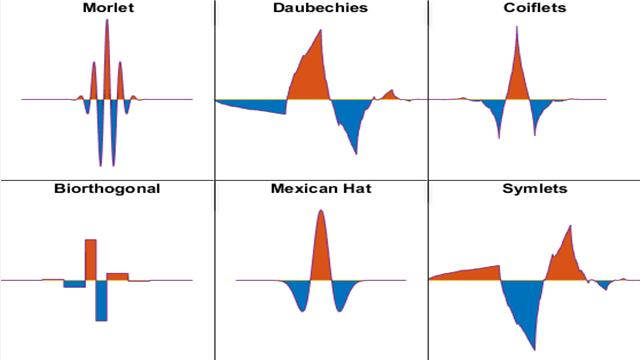
\includegraphics[width=13cm,center,keepaspectratio]{figures/wavelets}
\caption{Wavelet families \cite{fig:wavelets}}
\label{fig:wavelets}
\end{figure}
\subsection{Continuous wavelet transform}
The formula for the continuous wavelet transform is:
\begin{equation}
\textbf{CWT}^\psi_\chi(\tau,s) = \Psi^{\psi}_{\chi}(\tau,s) = \frac{1}{\sqrt{\left|s\right|}}\int x(t) \psi ^{\ast} (\frac{t - \tau}{s})dt
\label{Eq:CWT}
\end{equation}
where $\tau $ is translation (location of the window) and $s$ is scale. $\psi ^{\ast} (\frac{t - \tau}{s})$ is the \textbf{mother wavelet} which we will explain further later. \\
The most significant difference between STFT and wavelets is that the width of the window is changed in wavelet analysis whereas the window used by STFT is fixed \cite{giurgiutiu_comparison_2003}. For local areas with high frequencies the window size will be shorter whereas for local areas with low frequencies the window size will be longer. 
The term \textbf{mother wavelet} gets its name by two important properties. Firstly, wavelet as it is a small wave (finite length), and mother because all functions with different regions of support stem from a main function, the mother wavelet. This means that mother wavelet acts as a prototype for generating other functions. The translation term is related to the location of  the window while it is shifting through the signal. Thus, translation term corresponds to the time information. As we can observe there is no frequency component in the Eq. \ref{Eq:CWT}. Instead, we have the scale parameter which is $\frac{1}{frequency}$. In terms of frequencies, low frequencies (high scales) correspond to a macroscopic information of the entire signal, whereas high frequencies (low scales) correspond to a microscopic detailed information of the signal. High scales (low frequencies) last for the entire duration of the signal while low scales (high frequencies) do not last for the entire duration of the signals but appear from time to time like short bursts.  \\
\subsection{Discrete wavelet transform}
The discrete wavelet transform (\ac{DWT}) is an implementation of the wavelet transform using a discrete set of the wavelet scales and translations obeying some rules. DWT is simply a sampled version of \ac{CWT}. The Discrete Wavelet Transform (\ac{DWT}) provides sufficient information for synthesis and analysis of the original signal. \ac{DWT} is similar to the Fourier transform in that it is a decomposition of a signals in terms of a basis set of functions. In Fourier Transform, the basis set consists of sines and cosines and the expansions has one parameter which is the window length. In wavelet transform, the expansion has two parameters and the wavelets are generated from a single mother wavelet using dilation and offsets corresponding to the two parameters. The formula for the discrete wavelet transform is given by:
\begin{equation*}
f(t) = \sum_s\sum_{\tau} c_{s\tau} \psi_{s\tau} (t)
\end{equation*}
where the two-parameter expansion coefficients are given by
\begin{equation*}
c_{s \tau} = \int f(t) \psi_{s \tau}(t)dt
\end{equation*}
and the wavelets obey the situation
\begin{equation*}
\psi_{s\tau}(t) = 2^{\frac{s}{2}} \Psi(2^s t-\tau)
\end{equation*}
Here $\Psi$ is the mother wavelet, $s$ is the scale parameter and $\tau$ is the translate parameter. DWT applies the same idea as CWT. CWT is a correlation between a wavelet at different scales and the signal with the scale (or frequency) being used as a measure of similarity. By scaling the analysis window, shifting it in time, multiplying it and integrating it over all times, we acquire the CWT of a signal. \\
In the discrete case, filters of different cutoff frequencies are used to analyze the signal at different scales. The signal is passed through a series of high pass filters to analyze the high frequencies and it is passed through a series of low pass filters to analyze the low frequencies. The resolution of the signal, which is the amount of detail in the signal, is changed by the different filter operations and the scale is changed by the upsampling and the downsampling (subsampling). Subsampling a signal means that we reduce the sampling rate or removing some samples from the signal whereas upsampling means that we increase the sampling rate by adding new samples to the signal.
\begin{figure}[!htb]
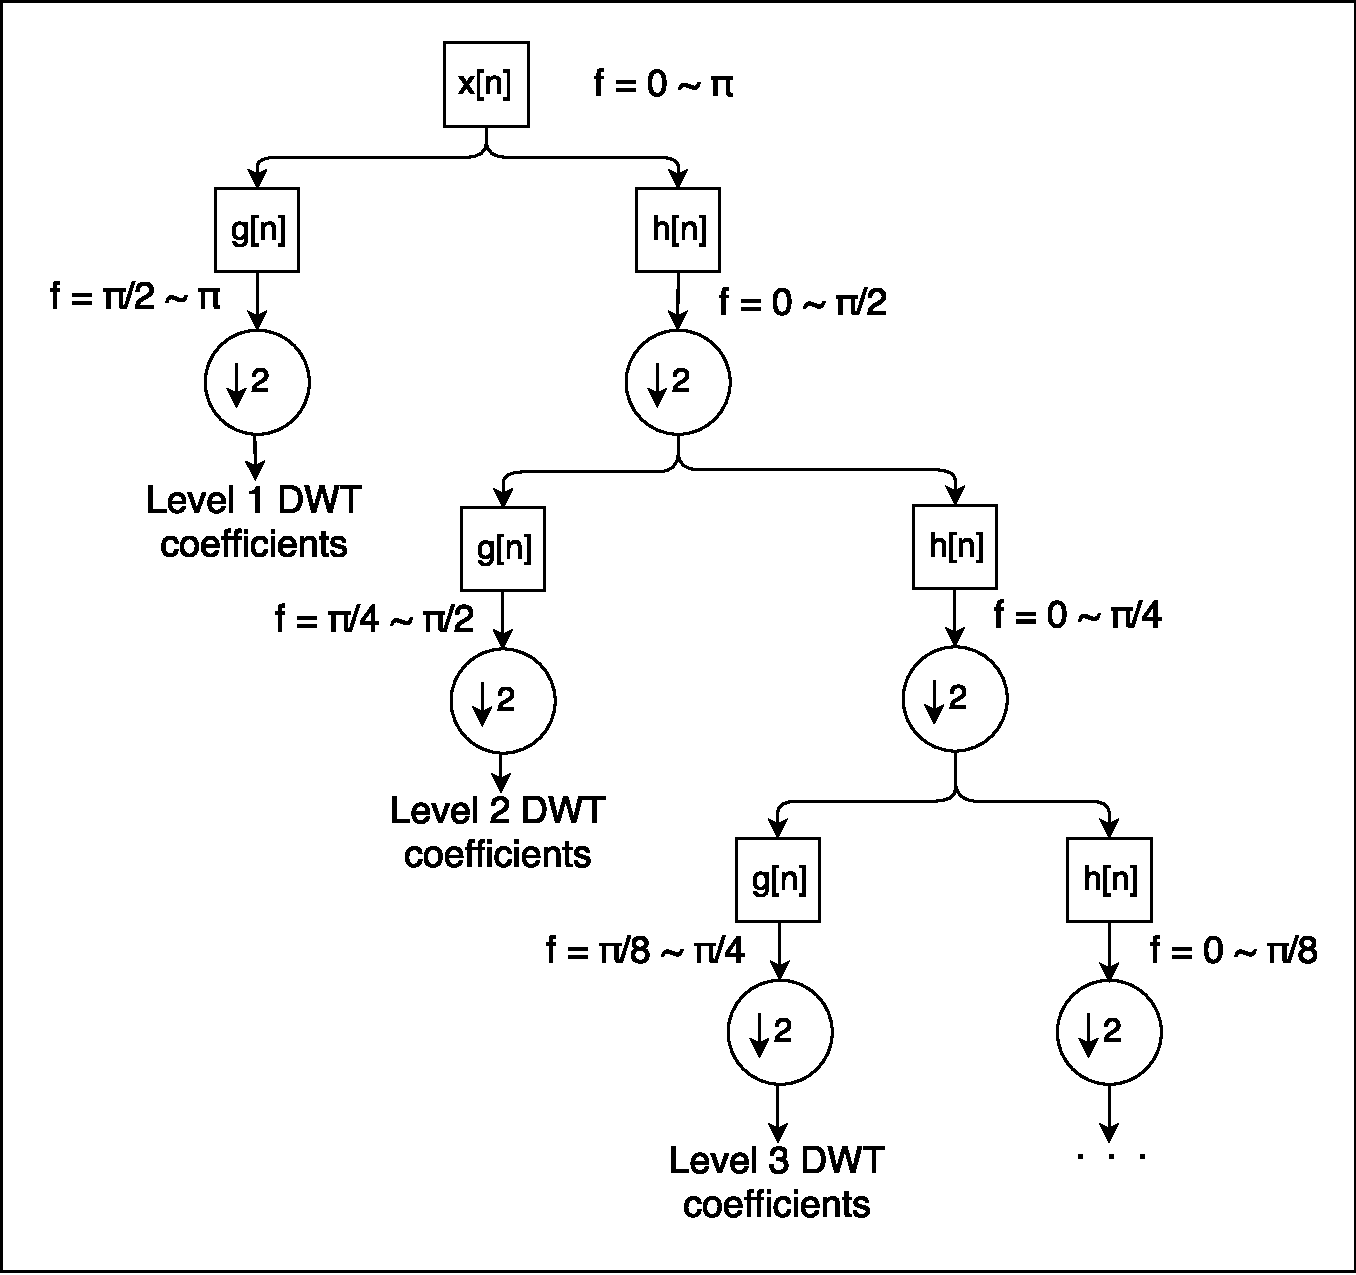
\includegraphics[width=15cm,left,keepaspectratio]{figures/subbandcoding}
\caption{The subband coding algorithm}
\label{fig:subbandcoding}
\end{figure}
The procedure starts with passing this signal through a half band digital lowpass filter with impulse response $h[n]$. The mathematical operation of convolution corresponds to filtering the signal with the impulse response of the filter. The convolution in discrete time is defined as:
\begin{equation*}
x[n] \circledast h[n] = \sum_{k=-\infty}^\infty x[k] \cdot h[n-k]
\end{equation*}
The half band lowpass filter removes all frequencies that are above half of the highest frequency in the signal. After passing the half band lowpass filter, half of the samples are eliminated thus leading to a subsampling of the signal by two, causing it to remain with half the number of points. Resolution is related to the amount of the information in the signal and therefore resolution is halved after the filtering operations. This causes the scale to double. This procedure can be expressed as:
\begin{equation*}
y[n] = \sum_{k=-\infty}^\infty h[k] \cdot x[2n-k]
\end{equation*}
According to the \ref{fig:subbandcoding} DWT employs two sets of functions, the scaling and the wavelet functions which correspond to low and highpass filters. These filters with the different frequency bands and with different resolutions, decompose the signal into a coarse approximation and detail information \cite{polikar_wavelet_1996}. The decomposition is obtained by applying successively highpass and lowpass filtering on the time domain signal.\\
The raw signal $x[n]$ is passed through a halfband highpass filter $g[n]$ and a lowpass filter $h[n]$. According to the Nyquist's rule, after the filtering, half of the samples are eliminated, since the signal has now a highest frequency of $p/2$ radians instead of $p$. This composes one level of decomposition and can be expressed as:
\begin{equation*}
y_{high}[k] = \sum_n x[n]g[2k - n]
y_{low}[k] = \sum_n x[n]h[2k - n]
\end{equation*}
where $y_{high}[k]$ and $y_{low}[k]$ are the outcomes of the highpass and lowpass filter after subsampling by 2.\\
Since only half of the number of the samples characterizes the raw signal, the decomposition halves the time resolution whereas the frequency resolution is doubled since the frequency band of the signal spans half the previous frequency band. At every level, the filtering and the subsampling half the number of samples (hence half the time resolution) and half the frequency band spanned (hence double the frequency resolution) \cite{polikar_wavelet_1996}. In the Fig. \ref{fig:subbandcoding} $h[n]$ $g[n]$ are lowpass and highpass filters and the bandwidth of the signal at every level is denoted with ``f''.\\
The most prominent frequencies in the raw signal will have the biggest amplitude in the DWT. The difference between DWT and the Fourier transform is that the time localization will be preserved. The time localization will have a different resolution depending on the current level we use for the DWT. The length of the signal determines the number of levels that the signal can be decomposed to. For example, if the signal length is 1024, ten levels of decomposition are possible \cite{polikar_wavelet_1996}. \\
If the main information is located in the high frequencies, the time localization will be more precise since higher frequencies are characterized by more number of samples. If the main information is located in the low frequencies, the time localization is less precise, since a small number of samples express the raw signal at low frequencies.\\
\subsubsection{Haar wavelet: An example of wavelet function}
The haar wavelet is the simplest kind of wavelet function. The haar wavelet is conceptually simple, memory efficient and computationally cheap. The haar transform also, does not have overlapping windows. Its formula is the following:
\[
\phi (t)
\begin{cases}
         1, & \text{if  } 0 \leq t \leq 1 \\
         0, & \text{otherwise}
\end{cases}         
\]
If we define the function $\psi(t)$ as $\psi(t) = \phi(2t) - \phi(2t-1)$, we can obtain the following function:
\[
\psi(t) = 
\begin{cases}
1, & \text{if } 0 < t \leq \frac{1}{2} \\
-1, & \text{if } \frac{1}{2} < t \leq 1 \\
0, & \text{otherwise }
\end{cases}
\]
The function $\phi(t)$ is the Haar scaling function, and $\psi(t)$ is the Haar wavelet. \cite{lee_wavelet_1994}
\subsection{Feature extraction in current work}
In Fig. \ref{fig:feature_extraction} we show that before proceeding with the preprocessing of the former matrix we created, we discard the time vector as we are not going to use the timestamps. Subsequently, we extract each 128-row-size segment from the matrix and we filter it with each feature we selected. After the feature extraction of each segment we convert the resulting matrix into a row. Each row represents the matrix from a preprocessed 128-row-size segment. The produced number of columns is variable for each different feature. We repeat all the aforementioned processes, for the data which are included in each of the folds. 
\begin{figure}[h!]
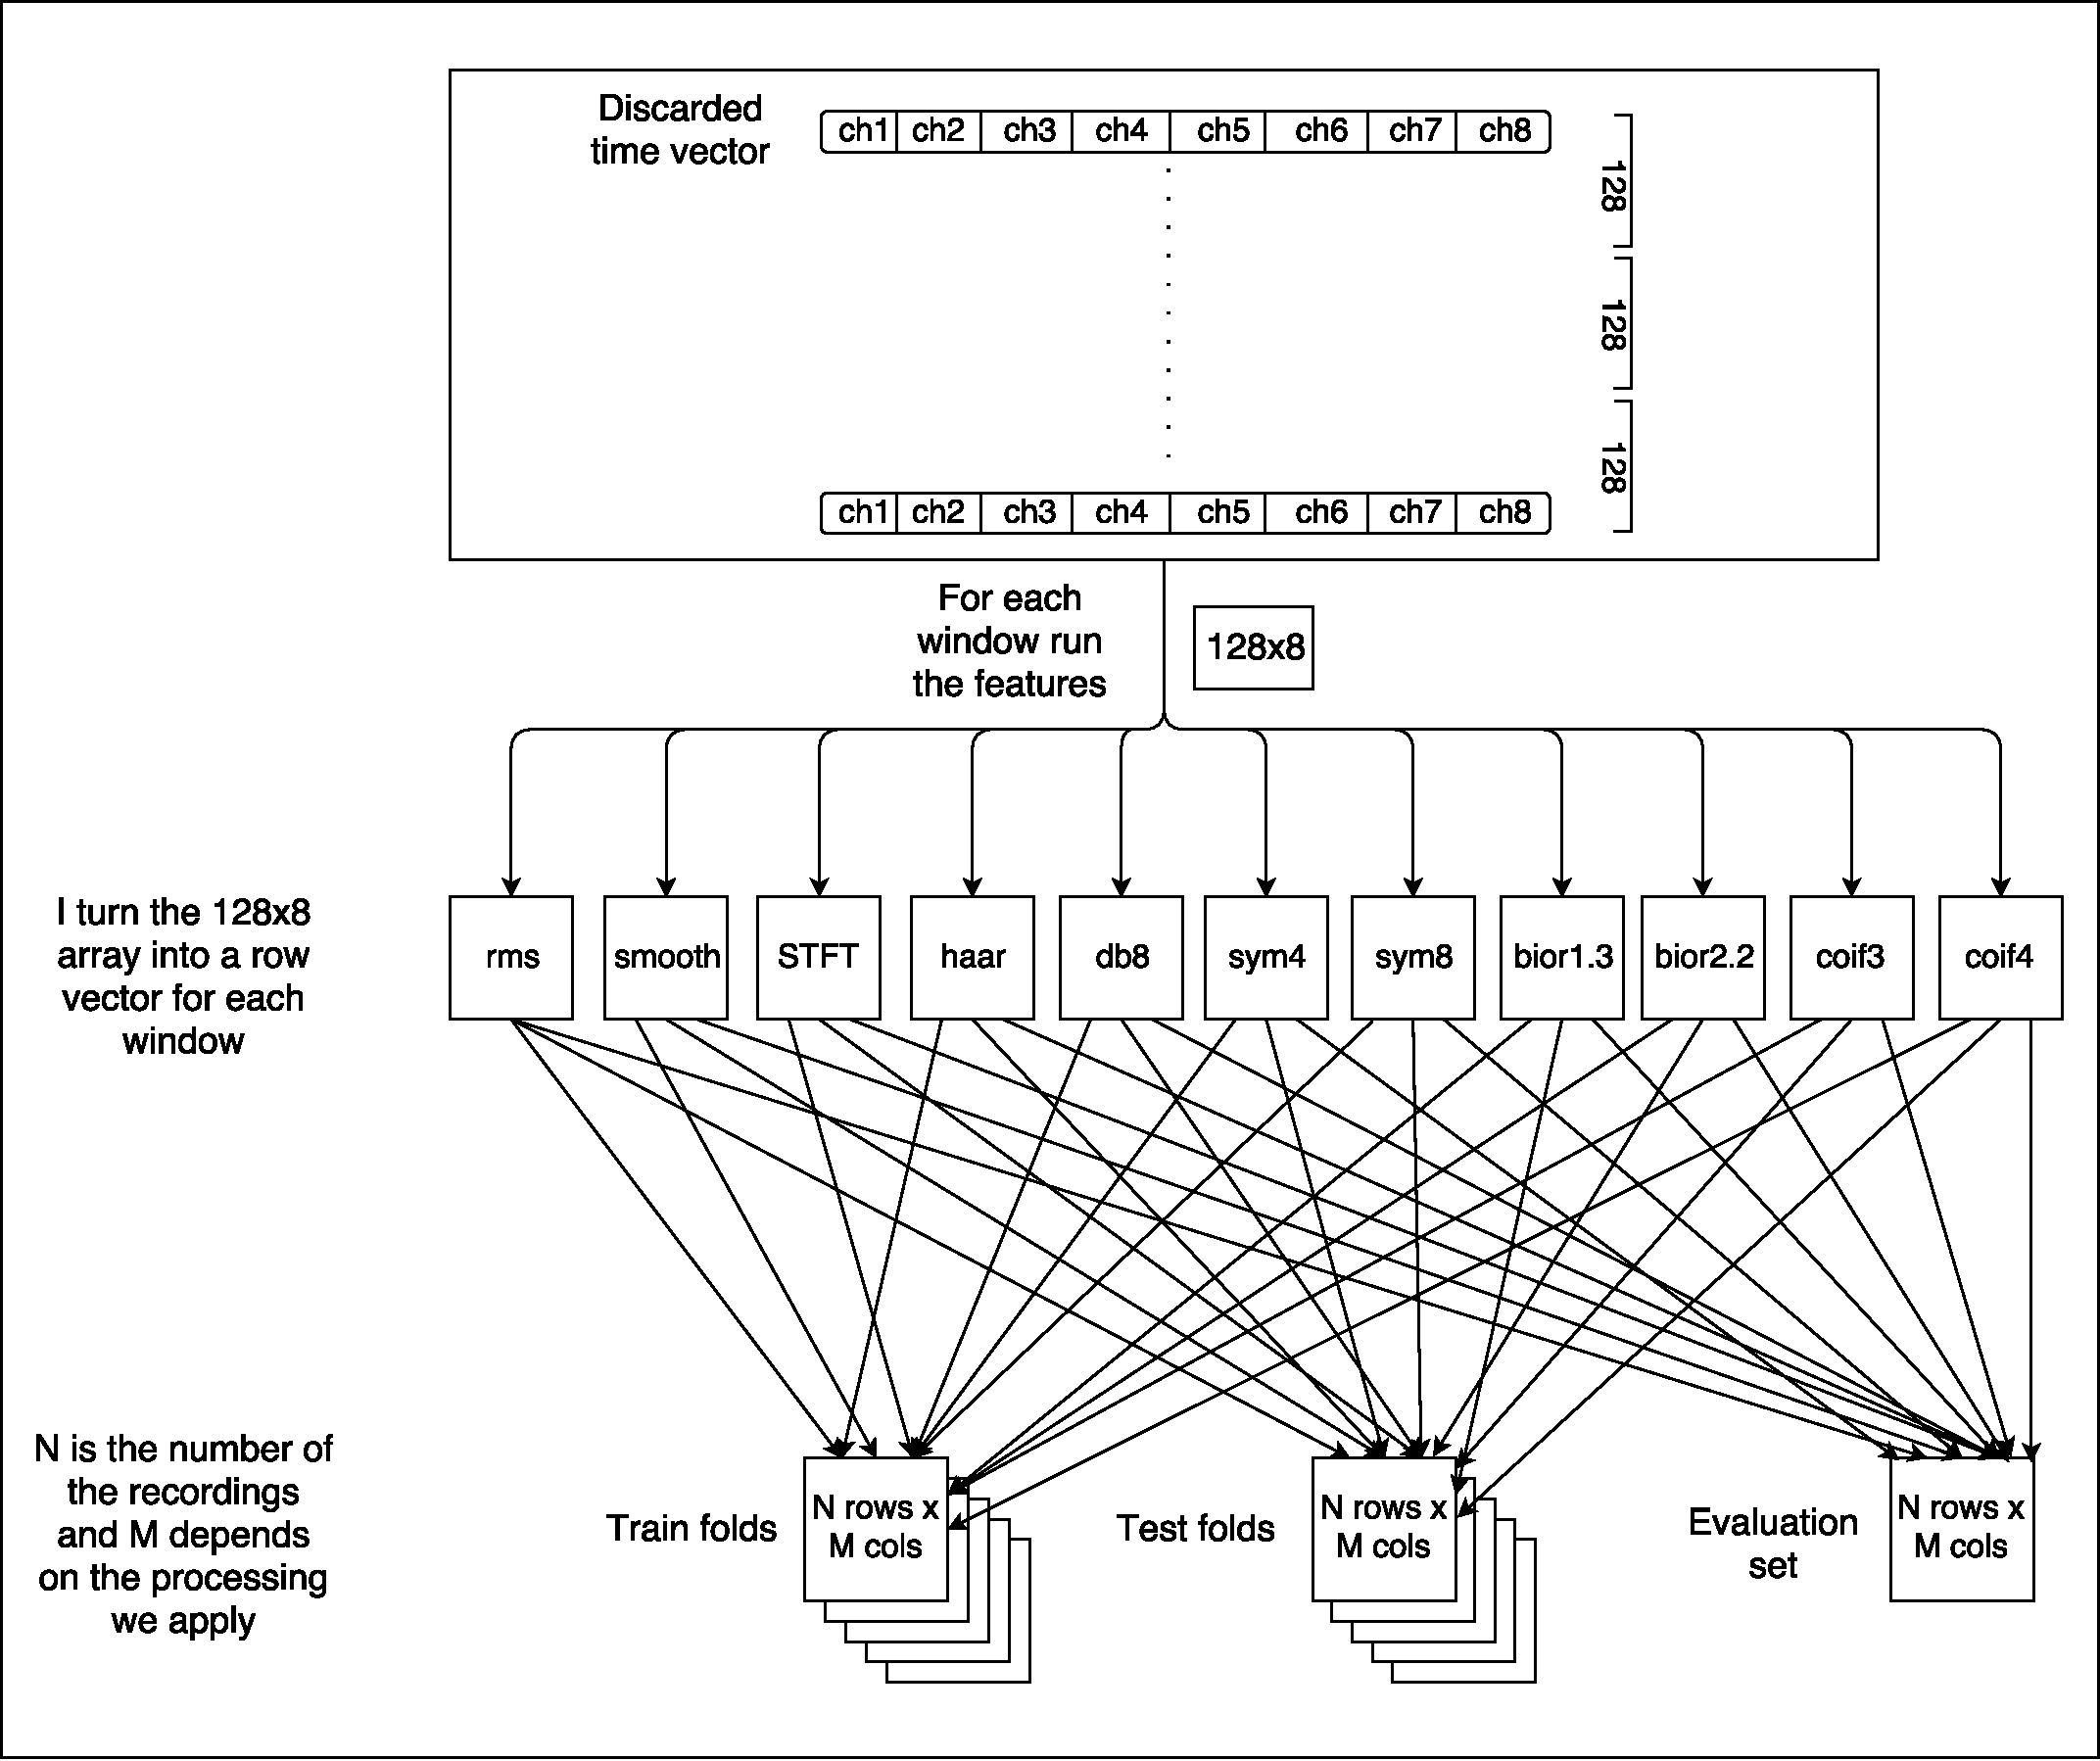
\includegraphics[width=15cm,left,keepaspectratio]{figures/feature_extraction}
\caption{Feature extraction}
\label{fig:feature_extraction}
\end{figure}
\section{Training and classification}
In Fig.\ref{fig:train_classification} we see that for each movement for feature from the train folds we train the SVM, \ac{ANN} classifiers. After the training has happened we use the test folds we previously created and we classify them with the newly trained network. After, that classification we calculate the accuracy which is calculated by the extraction of mean-squared-error from one.
\begin{figure}[h!]
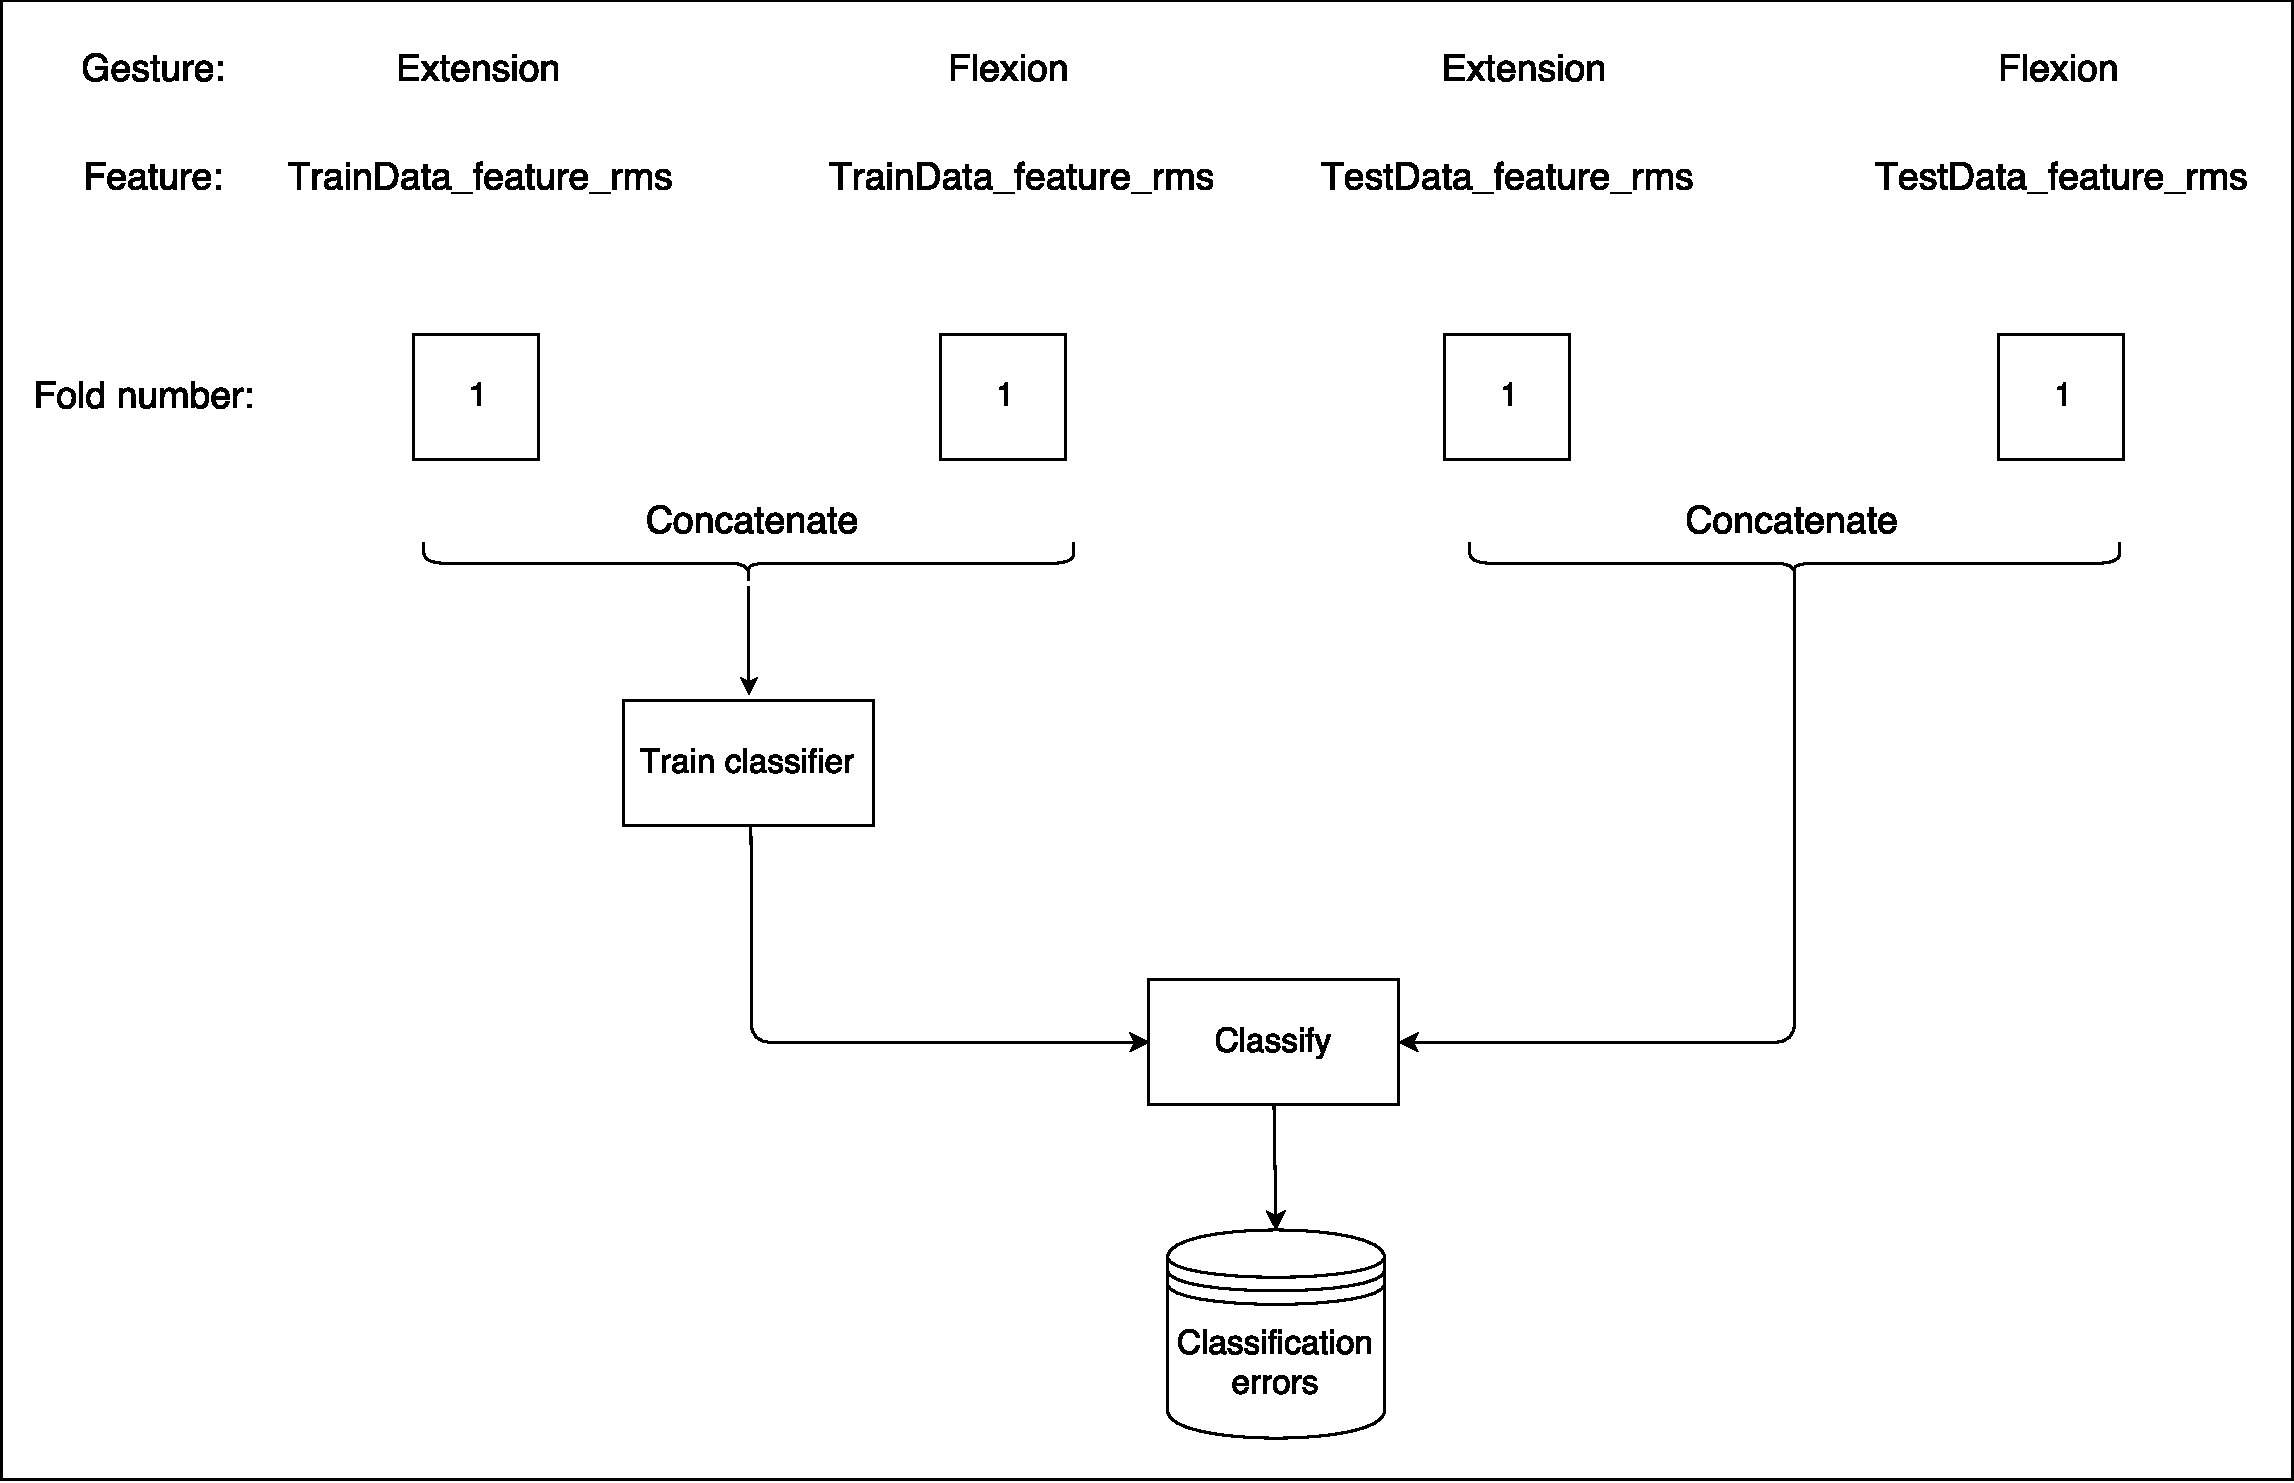
\includegraphics[width=15cm,center,keepaspectratio]{figures/train_classification}
\caption{Training \& classification: For the training part we concatenate the n-th training fold with the extension and the flexion data for each of the extracted features. We proceed by training the model with these data. Then, we concatenate the n-th test fold for the extension and flexion data and for the same feature as we did for the training folds. After testing the newly trained neural network with the test data we have the detection accuracies. }
\label{fig:train_classification}
\end{figure}
\subsection{Forward selection, backward elimination}
A common problem in pattern classification is to select a subset of features from a pool of many potential variables. As in most cases, in ours too, data acquisition process collects samples on a large number of variables because it is unknown which ones are the most important for class discrimination. To identify and select the most important and nonredundant variables from the large pool of potential variables is the goal of the feature subset selection \cite{mao_orthogonal_2004}.\\
In the work of Jovic et al. forward selection typically starts with an empty feature set and then considers adding one or more features to the set \cite{jovic_review_2015}.\\
In backward elimination, we typically start with the whole feature set and considers removing one or more features from the set.\\
Bidirectional search start from both sides, from an empty set and from the whole set, simultaneously considering larger and smaller feature subsets. Heuristic selection generates a starting subset based on a heuristic and then explores it further.\\
\section{Artificial intelligence}
Artificial intelligence (\ac{AI}) is a thriving field with many practical applications and current active research topics. AI tries to automate routine labor, understand speech or images, make diagnoses in medicine and support scientific research with the creation of intelligent software \cite{Goodfellow-et-al-2016}.\\
Artificial intelligence rapidly tackled and solved problems that are difficult for human beings but relatively straight-forward for computers, problems that can be described by a list of mathematical formulas. The demanding challenge for artificial intelligence is to solve tasks that are easy for people to solve but hard for them to describe formally, problems that we solve intuitively such as recognizing faces \cite{Goodfellow-et-al-2016}.\\
Computers have been able to defeat the best human chess players but only recently to recognize object or speech. A life of a person demands an immense amount of world knowledge. Much of this knowledge is subjective and therefore difficult to formally articulate. Thus, one of the key challenges in artificial intelligence is how to transfer this informal knowledge into the computer \cite{Goodfellow-et-al-2016}.\\
One solution is to create a knowledge base where we have to hard-code knowledge about the world formally. That will make the computer able to reason automatically about statements in languages that are designed to be used with logical inference rules. The disadvantage is that people struggle to describe everything about the world formally with logical rules \cite{Goodfellow-et-al-2016}.\\
This main disadvantage suggest that AI systems need the ability to acquire their own knowledge, by extracting patterns from data. This capability is also known as \textbf{machine learning}. The introduction of machine learning enable the computers to overcome problems that require knowledge of the real world and make decisions that appear subjective\cite{Goodfellow-et-al-2016}.\\
Many artificial intelligence  tasks can be solved by finding the right set of features to extract for that task, then providing these features to a simple machine learning algorithm such as logistic regression or naive Bayes. Although, for many tasks, is difficult to know what features should be extracted. \\
A way to improve machine learning with feature extraction is to use machine learning to discover the representation itself. This is known as representation learning. With this approach, the AI systems are enabled to adapt to new tasks faster with minimal human intervention. A representation learning algorithm can discover a good set of features for a complex task requires hours to months whereas the same complex task would require a great deal of time and effort.
\subsection{Biological and artificial neural networks}
The human brain is the most complex and most powerful organ of the human body. The inner functionality of the human brain is modeled around the \textit{neurons} and the networks of neurons known as \textit{biological neural networks}. The estimated number of human brain neurons is 100 billion, which are interconnected and communicate with one another through an interface consisting of \textit{axon terminals} that are connected to \textit{dendrites} across a gap (synapse) as shown in Fig. \ref{fig:biological_neuron}. 
\begin{figure}[h!]
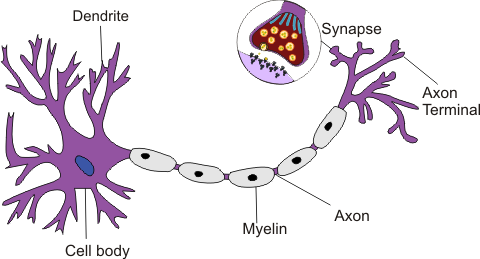
\includegraphics[width=10cm,center,keepaspectratio]{figures/biological_neuron}
\caption{Anatomy of a biological neuron \cite{fig:biological_neuron}}
\label{fig:biological_neuron}
\end{figure}
Simply put, the neuron will pass a message to another neuron across this interface if the sum of weighted input signals from one or more neurons exceeds a threshold to cause the message transmission. When the threshold is exceeded and the message is passed along to the next neuron is known as \textit{activation}.\\
An artificial neural network is basically a mathematical function. It is built from simple functions which have parameters which get adjusted. An example of such a function is shown in Fig. \ref{fig:artificial_neuron}. The below network takes $x_1$ to $x_n$ as numerical inputs and has weights $w_1$ to $w_n$ associated with these inputs. Additionally, there is another input $1$ with bias $b$ (called the bias) associated with it. There are thousands of those simple functions (also called ``neurons'') which build an artificial neural network. Each neuron's input signal is a weighted combination of many input signals and the weight of each input means that the input can have a different influence  on any subsequent calculations, und ultimately on the final output of the entire network. In addition, the main function of bias is to provide every node with a trainable constant value in addition to the normal inputs that the node receives. \\
\begin{figure}[h!]
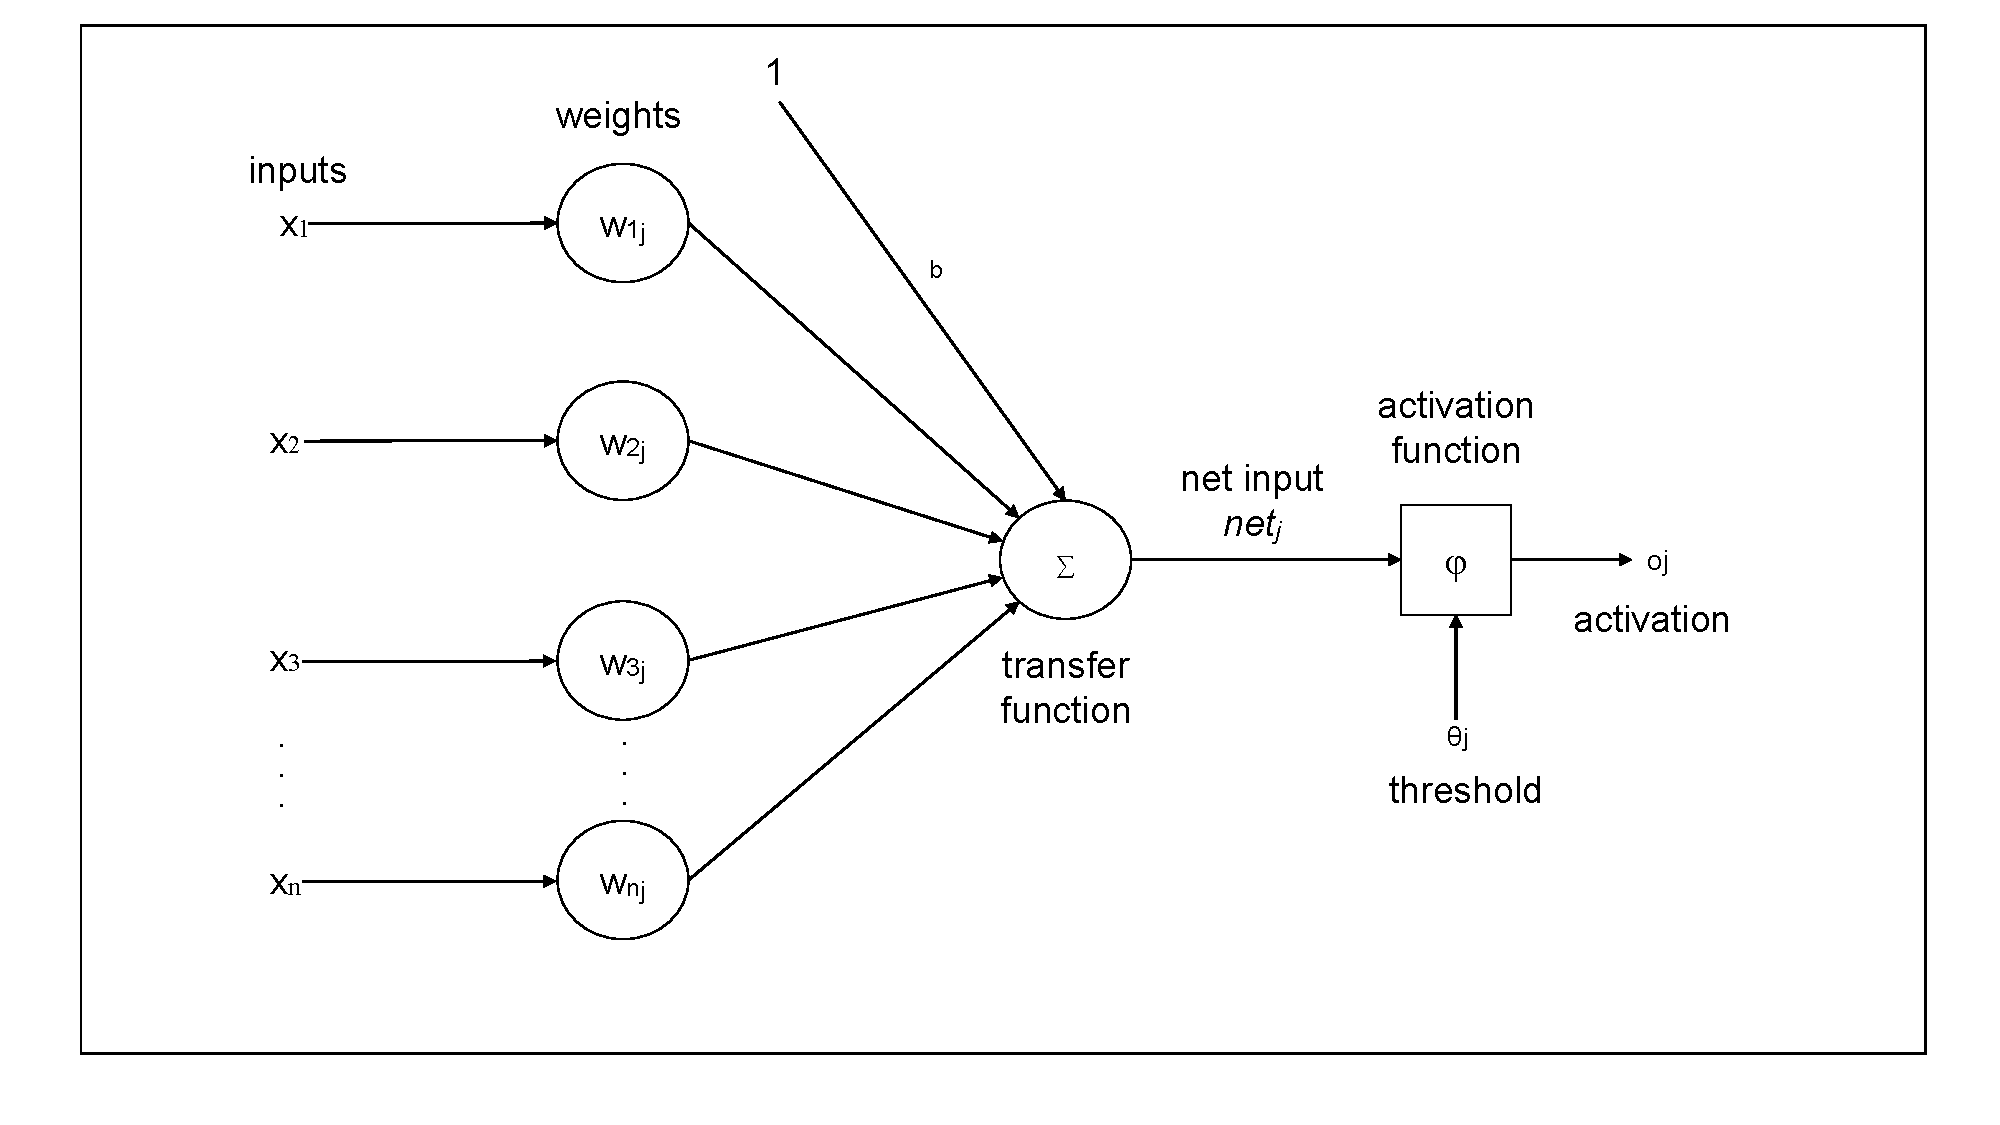
\includegraphics[width=15cm,center,keepaspectratio]{figures/artificial_neuron}
\caption{Artificial neuron}
\label{fig:artificial_neuron}
\end{figure}
Additionally, each neuron applies a transformation function to the weighted inputs, meaning that the summed weighted input signal is transformed mathematically prior to evaluating only if the activation threshold is exceeded. Here we list some of the several activation functions someone can encounter in practice: log-sigmoid, tan-sigmoid, the positive linear often referred to as rectified linear unit (ReLU) and the softmax tranfer functions which we will explain them later in detail. The combination of the weighted of input signals and the functions applied are typically either linear or nonlinear.\\
These input signals can originate in many ways, with our senses being some of the most important, as well as breathing, drinking and eating for example. A single neuron can receive hundreds of thousands of these input signals at once that undergo the summation process to determine if the message gets passed along and ultimately causes the brain to instruct actions, memory recollection and so on.\\
All the thoughts which are generated in our brains and the subsequent instructions given to our muscles, organs, and body are the results of these neural networks in action. The brain's neural networks continuously change and update themselves in many ways, including modifications to the amount of weighting applied among the neurons.\\
Ergo, it comes naturally to assume that, in order to transfer the brain's functionality and capabilities to  a computing machine, it must be implemented by a computer, artificial version of this network of neurons. This is the birth of this statistical processor and  known as \textit{artificial neural networks}. \\
\subsection{Artificial neural networks}
Artificial neural network is an interconnected group of natural or artificial neurons that uses a mathematical or computational model inspired by and modeled on biological neural networks. They are capable of processing nonlinear relationships between inputs and outputs in parallel. These networks are characterized by containing adaptive weights along the paths of many neurons which can be tuned by a learning algorithm which learns from observed data in order to improve the model. Apart from the learning algorithm, a cost function has to be chosen.\\
The cost function is used to learn the optimal solution to the problem being solved. It helps in determining the best values for all the tunable parameters, by adapting the weights along with other parameters such as the learning rate. These values are determined through optimization techniques such as gradient descent or stochastic gradient descent. These optimization techniques try to find the optimal solution, which when successful that means that ANN is able to solve the problem in question with a high accuracy. \\
Architecturally, an artificial neural network is modeled using layers  of artificial neurons, as shown in Fig. \ref{fig:artificial_neuron}, which are able to receive input and apply an activation function along with a threshold to determine if messages are passed along.\\
As shown in Fig. \ref{fig:simple_neural_network} the first layer in a neural network model is always the input layer followed by one hidden layer and lastly by an output layer. Each layer can contain one or more neurons. Models become increasingly complex by increasing the number of hidden layers, the number of neurons in any given layer or the number of paths between neurons. The following network is also known as feed-forward network. \\
\begin{figure}[h!]
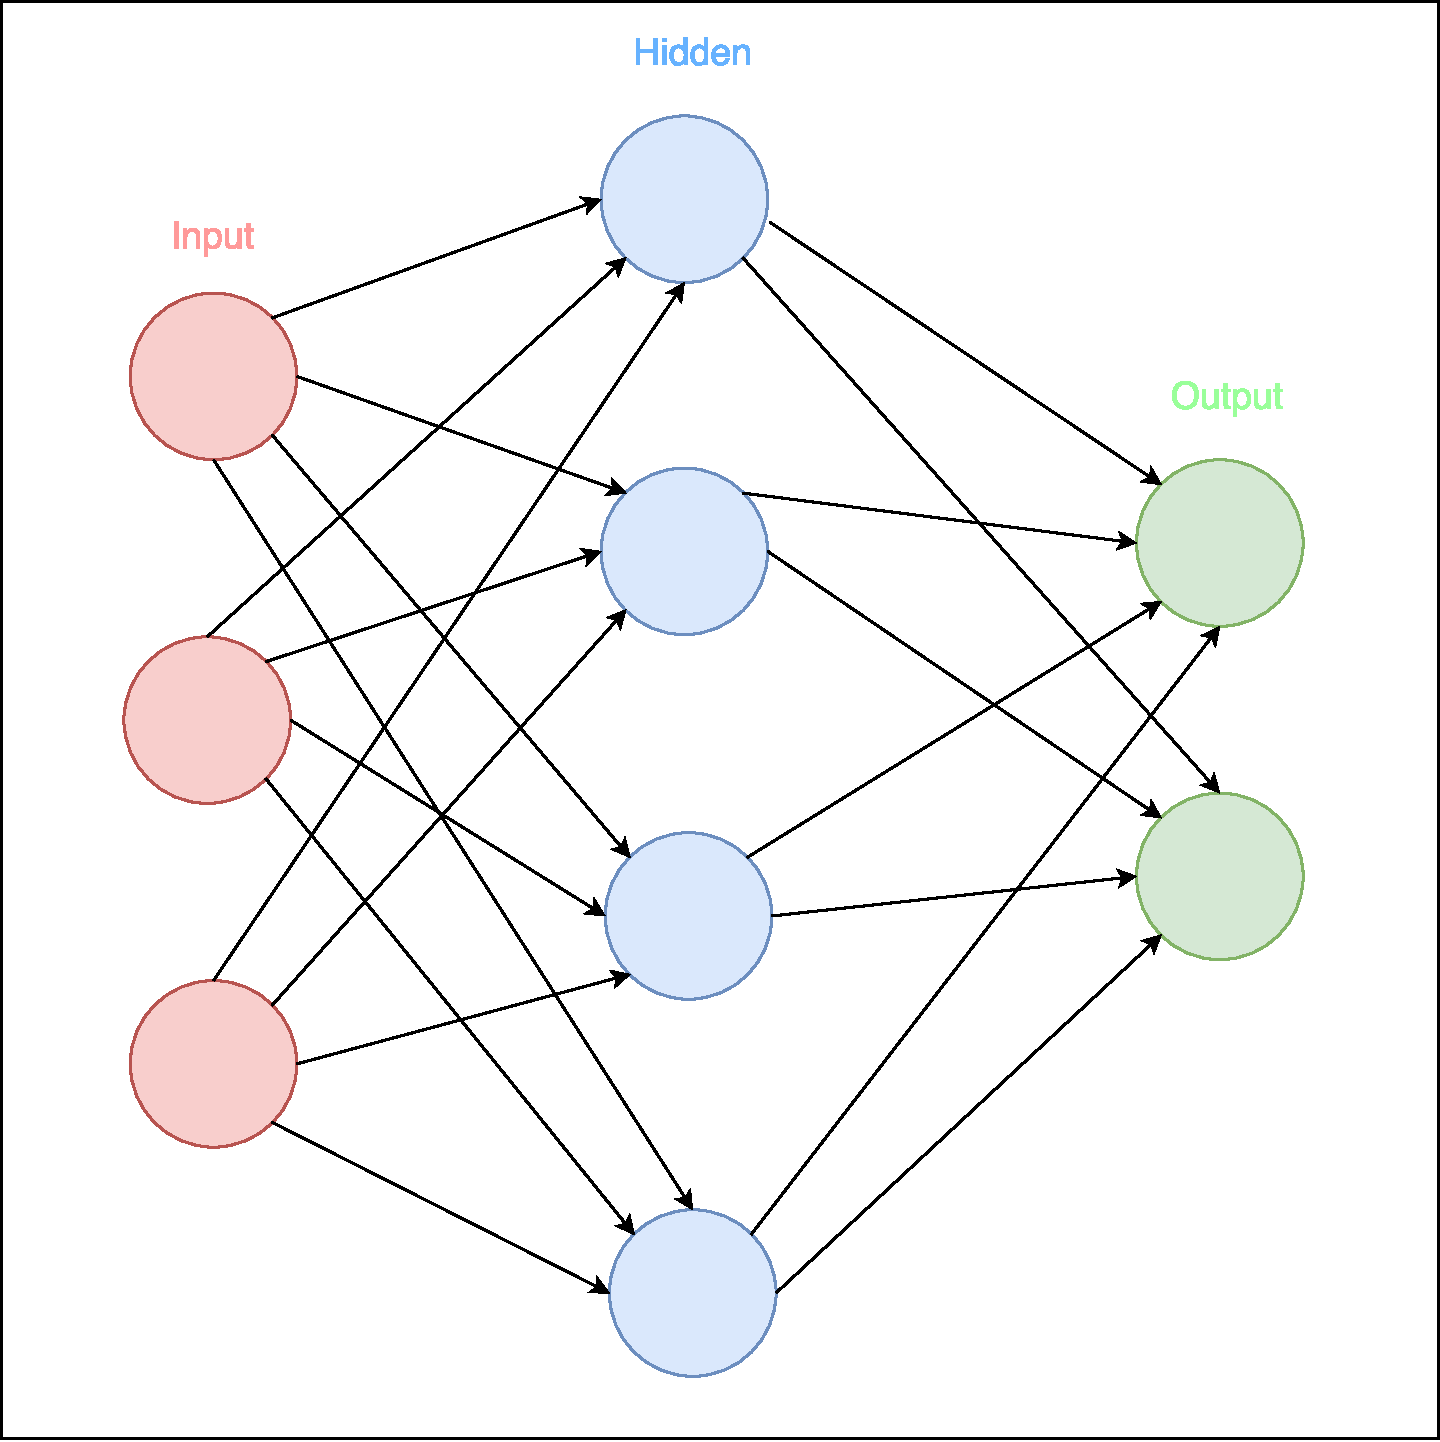
\includegraphics[width=10cm,center,keepaspectratio]{figures/simple_neural_network}
\caption{Feed-forward network}
\label{fig:simple_neural_network}
\end{figure}
Model architecture and tuning are therefore major components of ANN techniques in addition to the learning algorithms themselves. All of these characteristics of an ANN can have significant impact on the performance of the model.In addition, models are tuned by the activation function to convert a neuron's input to its output activation. \\
The meaning represented by a single artificial neuron is a form of local representation whereas the meaning of the entire neural network is a form of a distributed representation  due to the accumulated transformations across the neurons and layers.
\subsection{Deep learning}
Many machine-learning systems nowadays make an extended use of a class of techniques called deep learning. Deep learning also known as deep structured learning, is a branch of machine learning based on a set of algorithms that attempt to model high level abstractions in data. In a simple single-layer network we could have two sets of neurons: ones that receive an input signal and ones that send  an output signal. When the input layer receives an input it passes on a modified version of the input to the next layer. In a deep network, there are many layers between the input and the output, allowing the algorithm to use multiple processing layers, composed of multiple linear and non-linear transformations. \cite{Goodfellow-et-al-2016}\\
These methods have improved the state-of-the-art in speech recognition \cite{hinton_deep_2012}, object recognition \cite{girshick_rich_2014} and in other domains such as drug discovery \cite{gawehn_deep_2016} and genomics \cite{park_deep_2015}. The term ``Deep Learning'' was first introduced to machine learning by Dechter \cite{dechter_learning_1986}.
\subsection{Deep learning architecture}
We are going to list briefly the different deep learning architectures:
\begin{itemize}
\item \textbf{Generative deep architectures}, which are intended to characterize the high-order correlation of the observed or visible data for pattern analysis and characterize the joint statistical distributions of the visible data and their associated classes. \cite{dechter_learning_1986} Some of the types of generative models are hidden markov model and restricted boltzmann machine.
\item \textbf{Discriminative deep architectures}, which are intended to directly provide discriminative power for pattern classification, often by characterizing the posterior distributions of classes conditioned on the visible data. Some types of discriminative architecture are support vector machines, logistic regression which is a type of generalized of linear regression which is used for predicting binary or categorical outputs. 
\item \textbf{Hybrid deep architectures}, where the goal is discrimination but is assisted with the outcomes of generative architectures via better optimization and regularization, or discriminative criteria are used to learn the parameters in any of the deep generative models is the generative deep architectures category. \cite{deng_three_2012}
\end{itemize}
\subsection{Deep feed forward networks}
Deep feed-forward networks, also called feed-forward neural networks, or multilayer perceptrons (\ac{MLP}), are the quintessential deep learning models.\\
The goal of a feed-forward network is to approximate some function f$^{*}$ . For example, for a classifier, $y = f ^{*} (x)$ maps an input $x$ to a category $y$. A feedforward network defines a mapping $y = f(x;\theta)$ and learns the values of the parameters $\theta$ that result in the best function approximation.\cite{Goodfellow-et-al-2016}\\
In simple terms, the network can be defined as input, hidden and output nodes with data coming in from input node, processing is done in hidden nodes and then the output is produced  through the output nodes. The information  flows through the function being evaluated from $x$, through the intermediate computations used to define $f$, and finally to the output $y$. There are no feedback connections in which outputs of the model are fed back into itself and hence the models is called as feed-forward network. When feedforward neural networks are extended to include feedback connections, they are called recurrent neural networks. These kind of networks are used in many natural language applications \cite{mikolov_recurrent_2010}. The convolutional networks which are used for object recognition from photos are a specialized kind of feedforward network.\cite{Goodfellow-et-al-2016} \\
Deep feedforward networks also called \textbf{feedforward neural networks} or multilayer perceptronsare the most important deep learning models. Feedforward neural networks are called networks because they are typically represented by  composing together many different functions \cite{Goodfellow-et-al-2016}. The model is associated with a directed acyclic graph describing how the functions are composed together. For example, we might have three functions $f^{(1)},f^{(2)}$ and $f^{(3)}$ connected in a chain, to form $f(x) = f^{(3)}(f^{(2)}(f^{(1)}(x)))$. These chain structures are the most commonly used structures of neural networks. In this case, $f^{(1)}$ is called the first layer of the network, $f^{(2)}$ is called the second layer, and so on. The overall length of the chain gives the depth of the model. The name ``deep learning'' arose from this terminology. The final layer of a feedforward  network  is called the output layer. During neural network training, we drive $f(x)$ to match $f^{*}(x)$. The training data evaluate $f(x)$ with noisy, approximate examples of $f^{*}(x)$ at different training points. Each example $x$ is accompanied by a label $y \approx f^{*}(x)$. The training examples specify directly what the output layer must do at each point $x$; it must produce a value that is close to $y$. The learning algorithm must decide how to use those layers to produce the desired output, but the training data do not determine what each individual layer is expected to do. Instead, the learning algorithm must decide  how to use these layers to best implement an approximation of $f^{*}(x)$. Because the training data does not show the desired output for each of these layers, they are called \textbf{hidden layers}. \cite{Goodfellow-et-al-2016}\\
As these networks are inspired by neuroscience these networks are called neural. Each hidden layer of the network is vector valued. The dimensionality of these hidden layers determines the width of the model. Each element of the vector can be interpreted as playing a role analogous to a neuron. Rather than thinking of the layers as representing a single vector-to-vector function, we can imagine the layer as consisting of many inputs that act in parallel, each representing a vector-to-scalar function. Each unit resembles a neuron in the sense that it receives input from many other units and computes its own activation value. The idea of using many layers of vector-valued representations is originating from neuroscience.  The choice of the functions $f^{(i)}(x)$ used to compute these representations is also guided by neuroscientific observations about the functions that biological neurons compute. It is best to think of feedforward networks as machines that try to approximate functions which are designed to achieve statistical generalization.  \cite{Goodfellow-et-al-2016}\\
Linear models can help us to find a way to understand feedforward networks. Linear models such as logistic regression and linear regression, are appealing  because they can be fit efficiently and reliably. Linear models also have the obvious defect that the model is limited to linear functions, so the model cannot understand the interaction between any two input variables. \\
To represent nonlinear functions of $x$, we can apply the linear model not to $x$ itself but to a transformed input $\phi(x)$, where $\phi$ is a nonlinear transformation. We can think of $\phi$ as providing a set of features describing $x$, or as providing a new representation for $x$. 
The question arises on how to choose the mapping $\phi$.
\begin{itemize}
\item One option is to use a generic $\phi$. If $\phi(x)$ has high dimension, we can have enough capacity to fit the training set, but generalization to the test set remains poor. Very generic feature mappings are usually based only on the principal of local smoothness and do not encode enough prior information to solve advanced problems. \cite{Goodfellow-et-al-2016}
\item Another way is to manually configure $\phi$. Till the advent of deep learning, this was the dominant approach. It requires a lot of human effort for each separate task, with practicioners in different domains, such as speech recognition of computer vision.\cite{Goodfellow-et-al-2016}
\item The strategy of deep learning is to learn $\phi$. In this approach, we have a model $y = f(x;\theta,w)= \phi(x;\theta)^T w $. $\theta$ parameter is used to learn $\phi$ from a broad class of functions, and parameter $w$ that map from $\phi(x)$ to the desired output. This is an example of a deep feedforward network, with $\phi$ defining a hidden layer. In this approach, we parameterize the representation as $\phi(x;\theta)$ and use the optimization algorithm to find the $\theta$ that corresponds to a good representation. The advantage with this approach is that the human designer only needs to find the right general function family rather than finding precisely the right function.  \cite{Goodfellow-et-al-2016}\\
\end{itemize}
The general principle of improving models by learning features extends beyond the feedforward networks. Feedforward networks are the application of this principle to learnings deterministic mapping from $x$ to $y$ that lack feedback connections. Other models, apply these principles to learning stochastic mappings, functions with feedback and probability distributions over a single vector. \cite{Goodfellow-et-al-2016}\\
Last but not least, feedforward networks have introduced the concept of hidden layer, and this requires us to choose the activation functions that will determine the hidden layer values. We should also take into consideration about how many layers the network should contain, how these layers should be connected to each other and how many units should be in each layer. Learning in deep neural networks requires computing the gradients of complicated functions. The back-propagation is one of these algorithms which are used to compute these gradients. 
\subsection{Learning Conditional Statistics}
Instead of learning a full probability distribution $p(y |x;\theta)$, we want to learn just one conditional statistic of $y$ given $x$. For example, we may have a predictor $f(x;\theta)$ that we wish to employ to predict the mean of $y$. From this point of view, we can view the cost function as being a functional rather than just a function. A functional is a mapping from functions to real numbers. Therefore, we can think of learning as choosing a function rather than merely choosing a set of parameters. For example, we can design the cost functional to have its minimum lie on the function that maps $x$ to the expected value of $y$ given $x$. To solve the optimization problem with respect to a function requires a mathematical tool called \textbf{calculus of variations}. \cite{gelfand_calculus_2000}
Our first result derived using calculus of variations is that solving the optimization problem
\begin{equation}
f^{*} = argmin \mathbb{E}_{x,y \sim p_{data}}||y - f(x)||^2
\end{equation}
yields
\begin{equation}
f^*(x) = \mathbb{E}_{y \sim p_{data}(y|x)}[y] 
\end{equation}
so long as this function lies within the class we optimize over. To put it simply, if we could train on infinitely many samples from the true data generating distribution, minimizing the mean squared error cost function would give a function that predicts the mean of $y$ for each value of $x$.\\
Different cost functions give different statistics. A second result derived using calculus of variations is that:
\begin{equation}
f^* = arg min \mathbb{E}_{x,y \sim p_{data}}
\end{equation}
yields a function that predicts the median values of $y$ for each $x$, as long as such a function may be described by the family of functions we optimize over. This cost function is commonly called \textbf{mean absolute error}.\cite{Goodfellow-et-al-2016}\\
\subsection{Common Activation Functions}
When we construct an ANN model, on of the main consideration is to choose the proper activation function for hidden and output layers that are differentiable. The main reason behind that, is that when we calculate the backpropagated error signal that is used to determine ANN parameter updates requires the gradient of the activation function gradient. Four of the most common functions and their associated gradients are plotted in Fig.\ref{fig:activation_functions} :
\begin{figure}[h!]
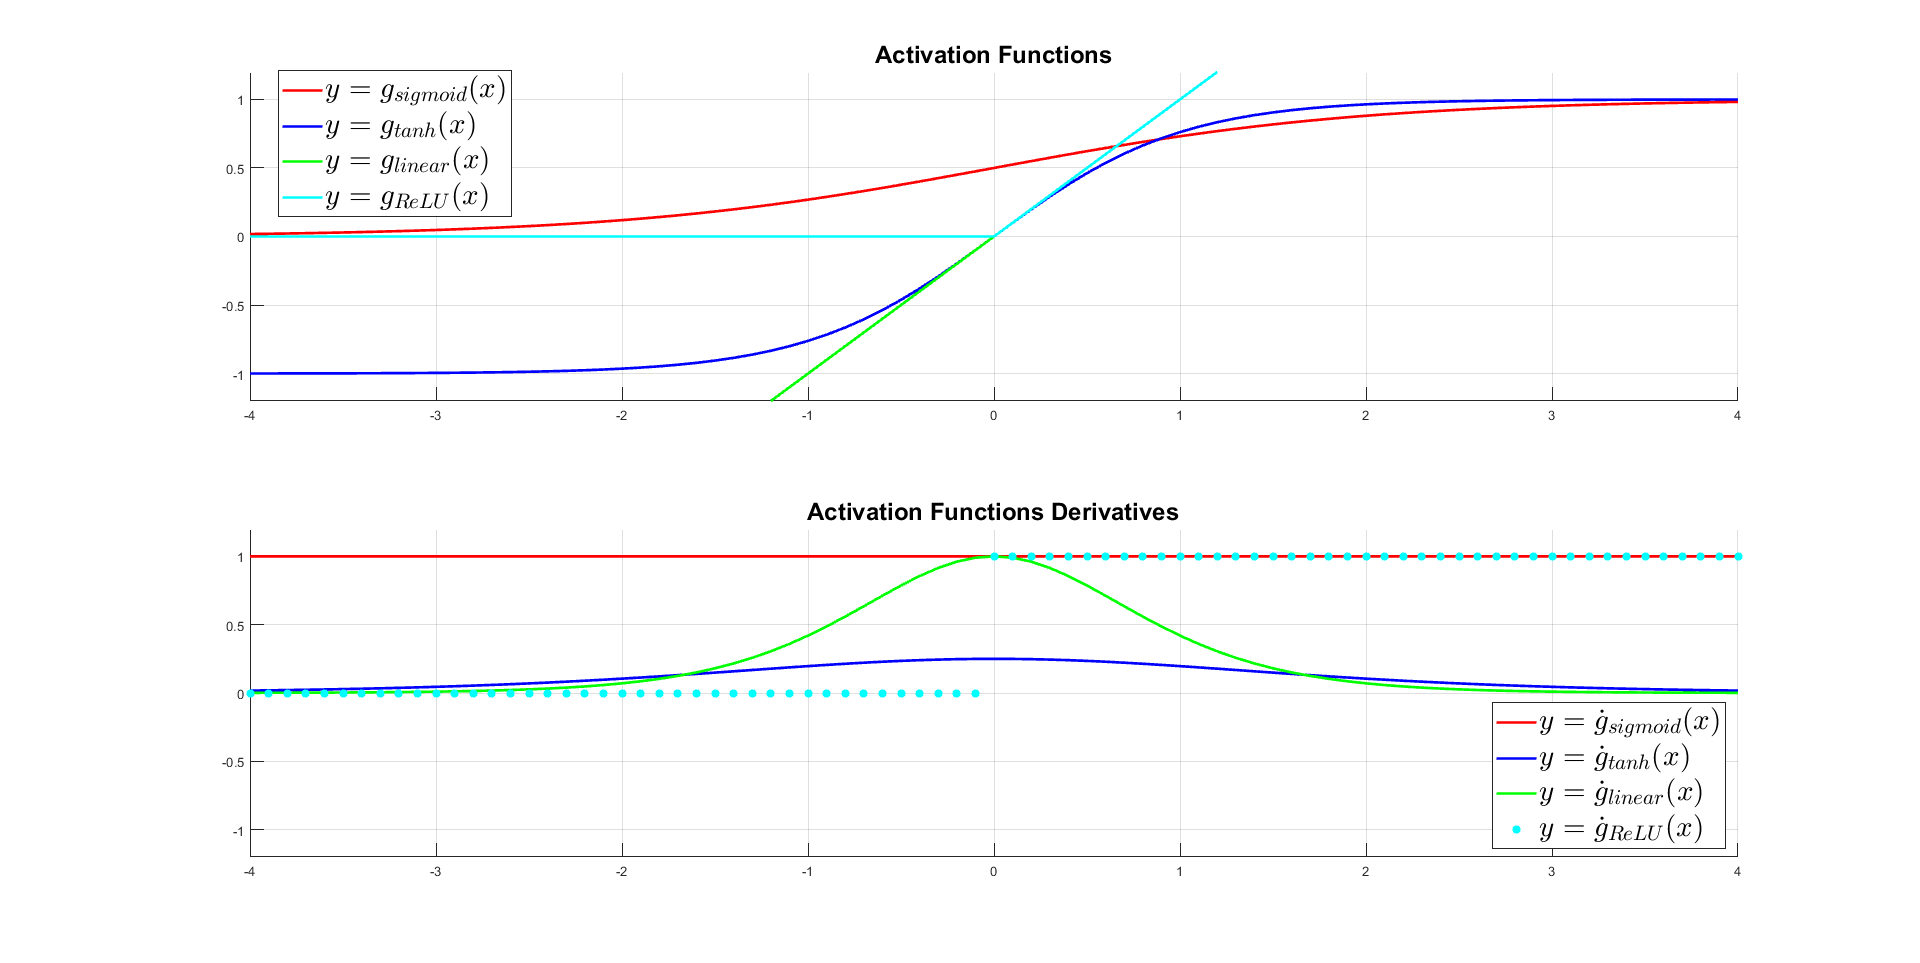
\includegraphics[width=20cm,center,keepaspectratio]{figures/activation_functions}
\caption{Common activation functions used in artificial neural networks along with their derivatives.}
\label{fig:activation_functions}
\end{figure}
\subsection{Identity Activation Function}
The simplest activation function, that is commonly used for the output layer in regression problems, is the identity/linear activation function:
\begin{equation*}
g_{linear}(z) = z
\end{equation*}
This activation function maps the pre-activation to itself and can output values that range $(-\infty,\infty)$. Even though, a multi-layered network with linear activations at each layer can be equally formulated as a single-layered linear network, the identity activation function seems to be extremely useful. In the case, where a multi-layered network that has nonlinear activations functions amongst the hidden units and an output layer  that uses the identity activation function implements a powerful form of nonlinear regression. \cite{Goodfellow-et-al-2016}
\subsection{Logistic Sigmoid}
A function that is often used as the output activation function for binary classification problems is the logistic sigmoid. The logistic sigmoid has the following form:
\begin{equation}
g(z) = \sigma (z) = \frac{1}{1 + \mathrm{e}^{-z}}
\end{equation}
and output values that range $(0,1)$. The logistic sigmoid can be interpreted as the probability of an artificial neuron ``firing'' given its inputs. Calculating the derivative of the logistic sigmoid makes use of the quotient rule:
\begin{equation}
\begin{split}
g'_{logistic} &= \frac{\partial}{\partial z}(\frac{1}{1+\mathrm{e}^{-z}})\\
          &= \frac{\mathrm{e}^{-z}}{(1+\mathrm{e}^{-z})^2}\\
          &= \frac{1 + \mathrm{e}^{-z} -1}{(1+\mathrm{e}^{-z})^2} \\
          &= \frac{1 + \mathrm{e}^{-z}}{(1+\mathrm{e}^{-z})^2} - (\frac{1}{1 + \mathrm{e}^{-z}})^2\\
          &= \frac{1}{(1+\mathrm{e}^{-z})} - (\frac{1}{1 + \mathrm{e}^{-z}})^2\\
          &= g_{logistic}(z) - g_{logistic}(z)^2\\
          &= g_{logistic}(z)(1 - g_{logistic}(z))
\end{split}
\end{equation}
This turns out to be convienient as we can see that $g'_{logistic}(z)$ evaluated at $z$ is $g_{logistic}(z)$ weighted by  $1-g_{logistic}(z)$ thus the gradients for the layers can be evaluated using simple multiplication and subtraction rather than performing any re-evaluating the sigmoid function, which requires extra exponentiation.\\
\subsection{Hyperbolic Tangent}
Although the logistic sigmoid has a biological interpretation, it turns out that the logistic sigmoid can cause a neural network to get ``stuck'' during training. In the case where a strongly-negative input is provided to the logistic sigmoid, it output values very near to zero. As we know, neural networks use the feedforward activations to calculate parameter gradients this affect the model parameters that are updated less regurarly than we would like and thus they are stuck in their current state.\cite{Goodfellow-et-al-2016} \\
An alternative to the logistic sigmoid is the hyperbolic tangent, or tanh function:
\begin{equation}
\begin{split}
g_{tanh}(z) &= \frac{sinh(z)}{cosh(z)}\\
			&= \frac{\mathrm{e}^z-\mathrm{e}^{-z}}{\mathrm{e}^z + \mathrm{e}^{-z}}
\end{split}
\end{equation}
As the logistic sigmoid, the tanh function is also sigmoidal but instead outputs values that range $(-1,1)$. Thus strongly negative inputs to the tanh will map to negative outputs. Additionally, zero-valued inputs are mapped to near-zero outputs. These properties make the network less likely to get ``stuck'' during training. Calculating the gradient for the tanh function also uses the quotient rule:
\begin{equation}
\begin{split}
g'_{tanh}(z) &= \frac{\partial}{\partial z}\frac{sinh(z)}{cosh(z)}\\
					&= \frac{\frac{\partial}{\partial z}sinh(z)cosh(z)-\frac{\partial}{\partial z}cosh(z)sinh(z)}{{cosh}^2(z)}\\
					&= \frac{{cosh}^2(z)-{sinh}^2(z)}{{cosh}^2(z)}\\
					&= 1 - \frac{{sinh}^2}{{cosh}^2}\\
					&= 1 - {tanh}^2(z)
\end{split}
\end{equation}
Similar to the derivative for the logistic sigmoid, the derivative of $g_{tanh}(z)$ is a function of feedforward activation evaluated at $z$, namely $(1 - g_{tanh}(z)^2)$.
\subsection{Rectified Linear Units}
Rectified linear units use the activation function $g(z) = max\{ 0,z \}$. These units are easy to optimize because they are similar to linear units. The only difference between a linear unit and a rectified linear unit is that a rectified linear unit outputs zero across half its domain. Therefore, this  makes the derivatives  through a rectified linear unit remain large whenever the unit is active. The gradients are not only large but also consistent. The second derivative of the rectifying operation is 0 almost everywhere, and the derivative of the rectifying operation is 1 everywhere the unit is active.\cite{Goodfellow-et-al-2016}\\
Rectified linear units are typically used on top of an affine transformation:
\begin{equation}
h = g(W^T x + b)
\end{equation}
When initializing the parameters of the affine transformation, it can be a good practice to set all elements  of b to a small positive value, such as 0.1. By doing so, it will be most likely that the rectified linear units will be active for most inputs in the training set and allow the derivatives to pass through. \\
When using a neural network to approximate a function, the data is forwarded through the network layer by layer until it reaches the final layer. The final layer's activations are the predictions that the network outputs. The essence of training our model  is to find the right set of weights for all the connections to make the right decision. To measure how well is our model performing we determine a metric which is also known as cost function. The discrepancies between the outputs in the estimations and the training set data are the principle values for our cost function. The goal of the training is to get the value of this cost function as low as possible.\cite{Goodfellow-et-al-2016}\\
\subsection{Softmax function}
The softmax transfer function is typically used as the transfer function for the output layer. It divides each output such that the total sum of the outputs is equal to one. The softmax function computes a categorical probability distribution that tells the probability that any of the classes are true. The mathematical formula for the softmax function is the following:
\begin{equation}
f{(z)}_i = \frac{e^{z_i}}{\sum_{j=1}^c e^{z}_j}
\end{equation}
In the above equation $z$ is a vector of the inputs to the output layer and $i$ indexes the output units.
\subsection{Minimization of the cost function}
One of the mostly used cost function is that of Mean-Squared-Error (\ac{MSE}) and we denote is as $J(W)$. 
\begin{equation}
J(W) = \frac{1}{m}\sum_{i=1}^m(h_W(x^{(i)})-y^{(i)})^2
\label{Eq:MSE_cost_function}
\end{equation}
where $m$ is the number of training examples, $x^{(i)}$ is the input vector for the $i^{th}$ training example and $y^{(i)}$ is the class label for the $i^{th}$ training example and $W$ are the chose parameter values or weights. Last but not least, $h_W(x^{(i)})$ is the algorithm's prediction for the $i^{th}$ training example using the parameters $W$.\cite{mccormickml}\\
We need to find the proper weights that will make the score of  this cost function as low as possible. Simply put we want to $\mathop{J(W)}_{\textbf{W}}$. To successfully minimize this function we need to take the first derivative and set it to zero and solve, which eventually will give us the locations of every minimum/maximum in this function. However, there are some difficulties with this approach:
\begin{itemize}
\item The cost function often is complex, so computing an expression for its derivative is time and resource consuming.
\item The cost function is also multi-dimensional and the need to find the points where all of those derivatives are zero is not trivial.
\item There is a large number of minima and maxima throughout the function and sorting out which one is the one we should be using is also computationally expensive. 
\end{itemize}
In addition to the aforementioned problems, as the size of networks begins to scale up, solving for the weights directly becomes increasingly infeasible. We overcome this problem by applying the so called iterative optimization algorithms which progressively work their way towards the optimal solution.\\
The most basic of the iterative optimization algorithms is the gradient descent. Generally, the cost function should be more or less convex, as Fig. \ref{fig:3D_convex_function} shows. To be truly convex however it is almost impossible. For the sake of simplicity, we need this example in order to explain how gradient descent works. \\
We start off by initializing our weight randomly, which puts us at the red as the Fig. \ref{fig:3D_convex_function} shows.
\begin{figure}[h!]
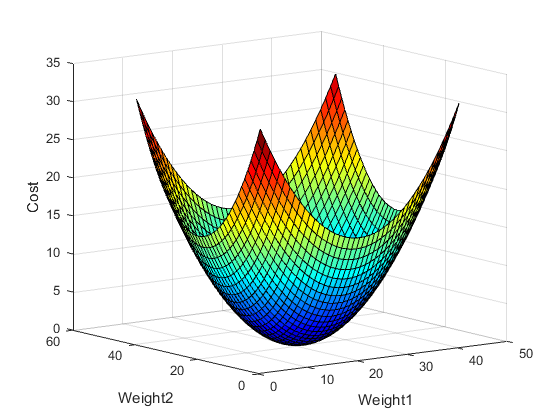
\includegraphics[width=10cm,center,keepaspectratio]{figures/3D_convex_function}
\caption{Convex function $z = x^2 + y^2$}
\label{fig:3D_convex_function}
\end{figure}
Taking the derivative, we see the slope at this point is a large positive number. Thus, we want to move closer to the center therefore we should take a large step in the opposite direction of the slope. If we repeat this process, eventually we will find the minimum of the curve as shown in Fig.\ref{fig:2D_convex_function} and much closer the optimal weight configuration for our model.
\begin{figure}[h!]
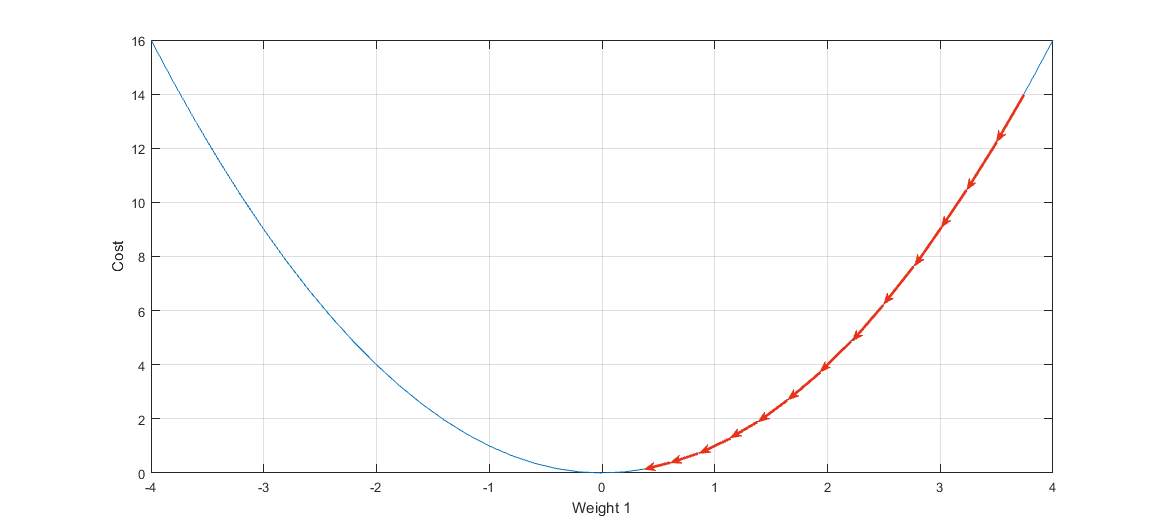
\includegraphics[width=16cm,center,keepaspectratio]{figures/2D_convex_function}
\caption{Convex function $y = x^2$}
\label{fig:2D_convex_function}
\end{figure}
The formula of gradient descent is as follows:
\begin{equation}
W := W - \alpha \frac{\partial J}{\partial W}
\end{equation}
where $\alpha$ is a parameter called  the learning rate. For example, we assume that we have as a cost function $J(W) = W^2$. We want to find the value of $W$ which minimizes $J(W)$. Let's assume that we start with $W=3$ and $\alpha = 0.1$. By doing simple calculations the Table \ref{table:gradient_descent_case} expresses how the value of $J'(W) = 2W$ changes and approaches to zero.
\begin{table}[h!]
\centering
{\rowcolors{2}{blue!10}{blue!20}
\renewcommand{\arraystretch}{1.3}
\begin{tabular}{ |p{2.5cm}|p{2.5cm}|p{2.5cm}|  }
\hline
Iteration & $W$ & $\alpha \frac{\partial J}{\partial W}$ \\
\hline
1 & 3     & 0.6 \\
2 & 2.4   & 0.48 \\
3 & 1.92  & 0.384 \\
4 & 1.536 & 0.307 \\
5 & 1.229 & 0.246 \\
6 & 0.983 & 0.197 \\
7 & 0.786 & 0.157 \\
8 & 0.629 & 0.126 \\
9 & 0.503 & 0.101 \\
10 & 0.403 & 0.081 \\
\hline
\end{tabular}
}
\caption{The values of W prior to each iteration and the update amounts.}
\label{table:gradient_descent_case}
\end{table}
As can be seen in our simple example, every time the weights are updated, there is a subtraction of the cost function with respect to the weight scaled by the learning rate $\alpha$. Thus, leads to the derivative term getting smaller and smaller and converging near to zero. Also, selecting the right learning rate is critical. If the learning rate is too large, we can overstep the minimum and diverge. On the contrary, if we choose a too small value for the learning rate we need to run more iteration of gradient descent and this will lead to the increase of the training tim \cite{mccormickml}.\\
In the above example we examined the case of a single variable cost function. Additionally to the single variable cost function we can have two or more variables in the cost function. Let's examine the case of the function $J(W) = W_1^2 + W_2^2$. This convex function is shown in Fig. \ref{fig:3D_convex_function}. When there are multiple variables in the minimization objective, gradient descent defines a separate update rule for each variable. Let's try to show mathematically how the derivatives of the cost functions build up:
\begin{align*}
\frac{\partial}{\partial W_1}J(W_1,W_2) = \frac{\partial}{\partial W_1}{W_1}^2 + \frac{\partial}{\partial W_1} {W_2}^2 = 2W_1 \\
\frac{\partial}{\partial W_2}J(W_1,W_2) = \frac{\partial}{\partial W_2}{W_1}^2 + \frac{\partial}{\partial W_2} {W_2}^2 = 2W_2
\end{align*}
As we can see, when we take the partial derivative with respect to $W_1$ we treat $W_2$ as a constant.\\
We showed the MSE cost function in Eq. \ref{Eq:MSE_cost_function}. Similarly, with the previous derivatives let's develop the derivative of the MSE cost function:
\begin{align*}
\frac{\partial}{\partial W_0}J(W_0,W_1) &= \frac{\partial}{\partial W_0}(\frac{1}{m}\sum_{i=1}^m (h_W(x^{(i)})-y^{(i)})^2)\\
&= \frac{1}{m}\sum_{i=1}^m \frac{\partial}{\partial W_0}(h_W(x^{(i)})-y^{(i)})^2)\\
&= \frac{1}{m}\sum_{i=1}^m 2(h_W(x^{(i)})-y^{(i)})\frac{\partial}{\partial W_0}(h_W(x^{(i)})-y^{(i)})\\
&= \frac{2}{m}\sum_{i=1}^m(h_W(x^{(i)})-y^{(i)})
\end{align*}
Lastly, each update of the $W$ variables is averaged over the training set. Every training example suggests its own modification to the weight values and then we average these suggestions to make our actual update. This means that the statistics of our training set are being taken into account during the learning process. An outlier training example (mislabeled or corrupted one) is going to have less influence over the final weights. \cite{mccormickml} \\
\subsection{Backpropagation}
Before the backpropagation algorithm there were many other methods implemented to adjust the weights in a random, uninformed direction (ie. increase or decrease) and check if the performance of the ANN is increasing. If it did not increase, then one would attempt to either go in the other direction or reduce the perturbation size or combine both \cite{ayearofai}.\\
Backpropagation give us an understanding on how to change the weights and biases in a network to have the desired changes on the cost function. For other machine learning algorithms like logistic regression (the sigmoid function) or linear regression computing the derivatives is an elementary application of differentiation. The same, however, cannot be said for neural networks. To demostrate this, we will demonstrate a diagram of a double-layered neural network:
\begin{figure}[h!]
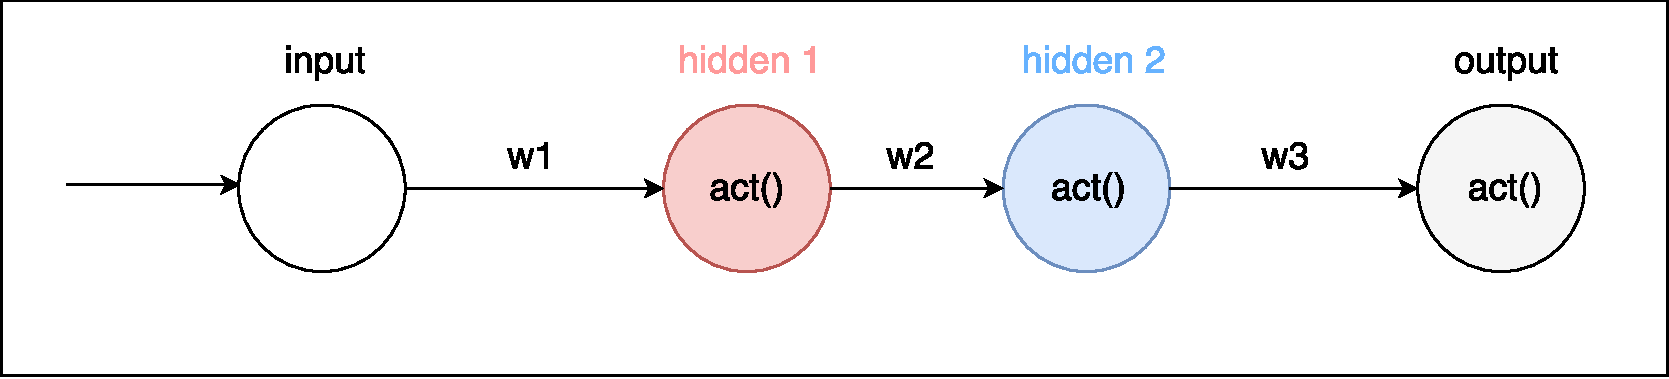
\includegraphics[width=15cm,center,keepaspectratio]{figures/double_layered_neural_network}
\caption{Double layered neural network}
\label{fig:double_layered_neural_network}
\end{figure}
In Fig. \ref{fig:double_layered_neural_network} we see that each neuron is dependent of the previous one connected to it. Put it simply, if we change the value of $w_1$, both ``hidden 1'' and ``hidden 2'' neurons (output layer inclusive) neurons will change. So we have the composite functions to compose the output function:
\begin{align*}
output &= act(w3 * hidden2)\\
hidden2 &= act(w2 * hidden1) \\
hidden1 &= act(w1 * input)
\end{align*}
Therefore we have:
\begin{equation}
output = act(w3 * act(w2*act(w1*input)))
\end{equation}
As we see, the output is a composite function of the weights, inputs and activation functions. Now, let's calculate the derivative  of this function with respect to the arbirtary weight for example $w1$. For this we have to apply the chain rule and we will have the following equation:
\begin{equation*}
\frac{\partial}{\partial w1}= \frac{\partial}{\partial hidden2}output* \frac{\partial}{\partial hidden1}hidden2 * \frac{\partial}{\partial w1}hidden1
\end{equation*}
If we are to compute the derivative of the error with any arbitrary weight the result equation will be:
\begin{equation*}
\frac{\partial error}{\partial w1}= \frac{\partial error}{\partial output}* \frac{\partial output}{\partial hidden2}* \frac{\partial hidden2}{\partial hidden1}*\frac{\partial hidden1}{\partial w1}
\end{equation*}
Each of these derivatives can be simplified once we choose an activation and error function as we discussed earlier. At this point, any abstraction has been removed, and the error derivative can be used in gradient descent to iteratively improve upon the weight. We compute the error derivatives according to every other weight in the network and apply gradient descent similarly. This procedure is called the backpropagation where the computation of the derivatives are fed to an optimization algorithm. The name backpropagation justifies the whole procedure as we are traversing from the output error to the weights, taking iterative steps using the chain rule until we reach the weight \cite{ayearofai}.\\
\subsection{Summary of training neural network}
We can summarize the steps of training an entire neural network:
\begin{enumerate}
\item Create our connected neural network and prepare training data
\item Initialize all the weights to random values. Here we have to emphasize we must not initialize the weights to zero. If weights are initialized to zero, the outgoing weights of each neuron will be identical because the gradients will be identical. Due to this, the proceeding hidden neurons will keep the same value and will continue to follow each other. This means that our neural network may get stuck at local optima. Therefore, random weight initialization allows us to overcome this problem by starting with many random values.\cite{ayearofai}
\item Perform one feed-forward using the training data
\item Perform backpropagation to get the error derivatives for each and every weight in the neural network
\item Perform gradient descent to update each weight of the respective error derivative.
\item If we have converged  training is complete. In reality most time, we stop when we have reached the number of maximum iterations. 
\end{enumerate}
\section{Data evaluation}
To test the optimal parameters for our neural network we need evaluation data. We created a new database with finger gestures consisted only from EMG signals. The signals were acquired with the Myo armband. The IMU data was discarded since there was no motion of the hand only motion of the fingers and keeping still the hand during the whole experiment. The 80\% percent of the new acquired data was used to train the neural nets and the rest 20\% was used to test the newly trained neural nets.\\
After the protocol for the new finger gestures was created and we created a database with the 14 new finger gestures and classify them into two classes: extension and flexion. We acquired new signals from the forearms of 21 subjects aged between 20-30. Below are the images with the extensions and the flexions of the gestures:
\begin{figure}
  \begin{subfigure}[t]{0.5\linewidth}
  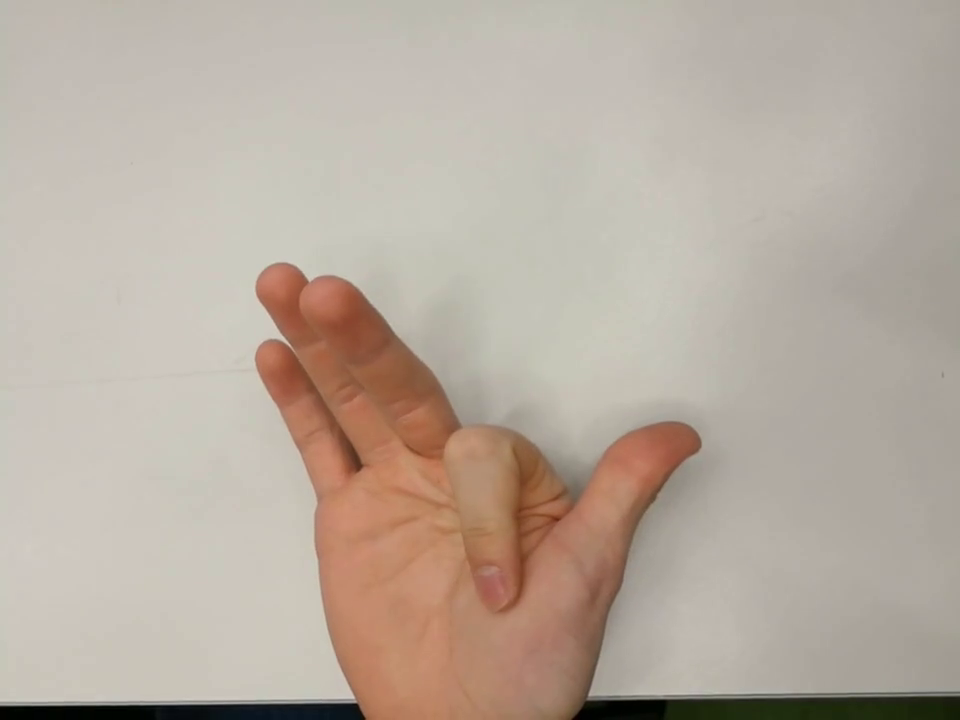
\includegraphics[width=100pt]{figures/ext_index1}
  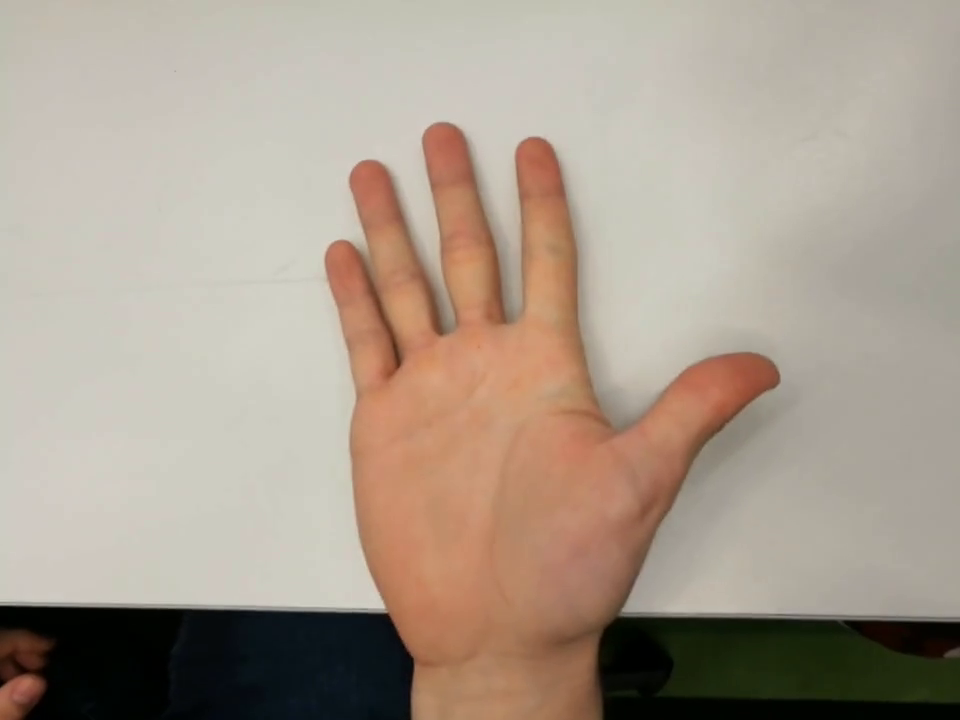
\includegraphics[width=100pt]{figures/flx_index1}
  \caption{G1: Index extension and flexion with the palm facing upwards}
  \end{subfigure}
  \hspace*{\fill}
  \begin{subfigure}[t]{0.5\linewidth}
  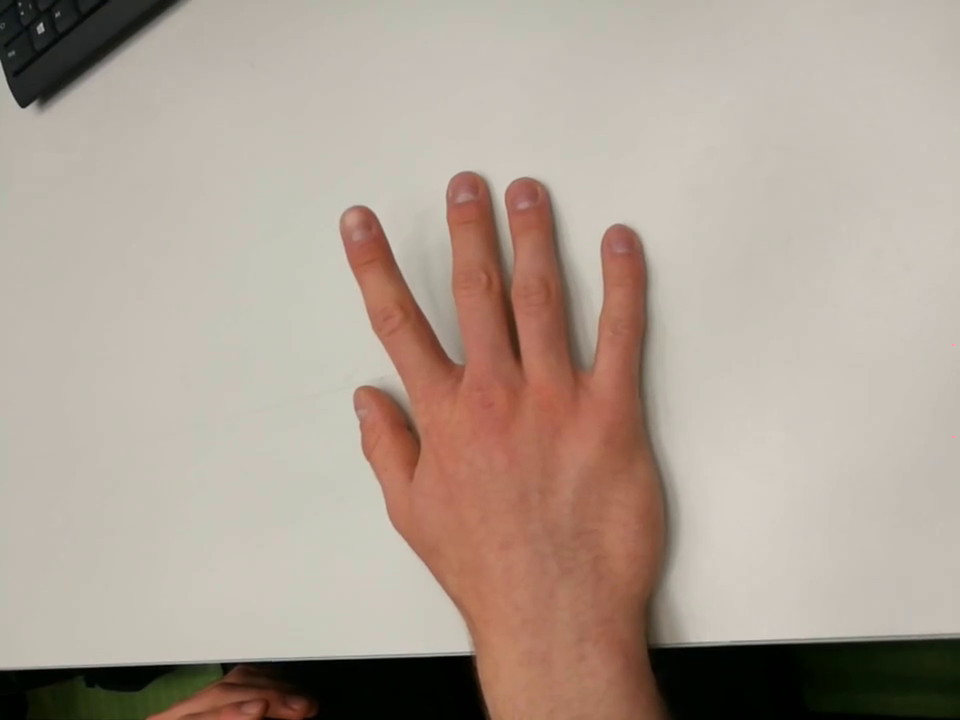
\includegraphics[width=100pt]{figures/ext_index2}
  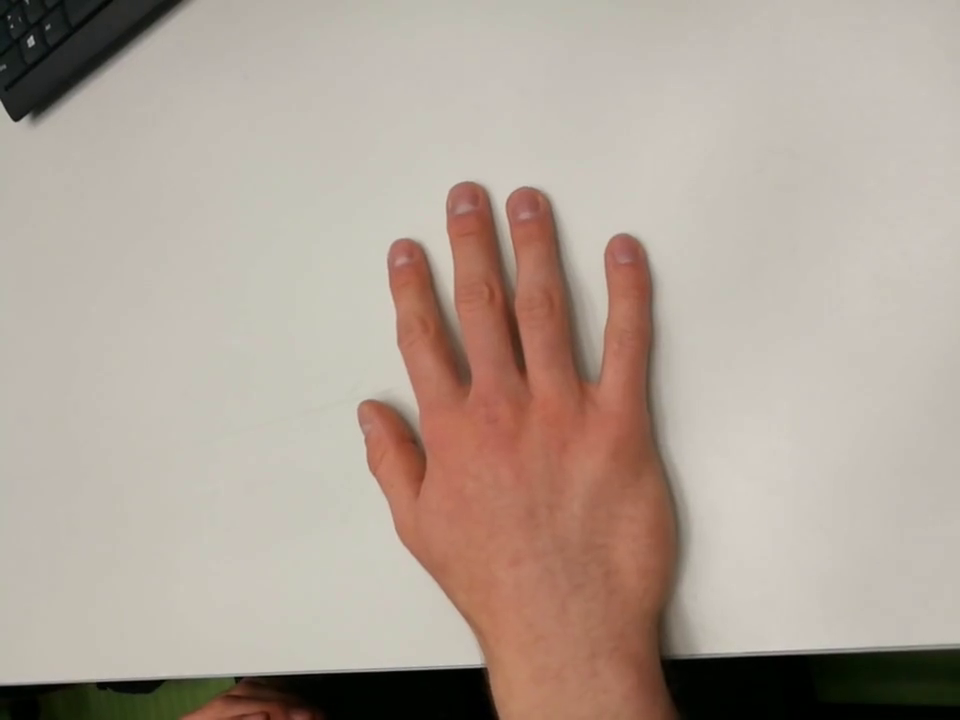
\includegraphics[width=100pt]{figures/flx_index2}
  \caption{G2: Index extension and flexion with the palm facing downwards}
  \end{subfigure}\par\medskip
  \begin{subfigure}[t]{0.5\linewidth}
  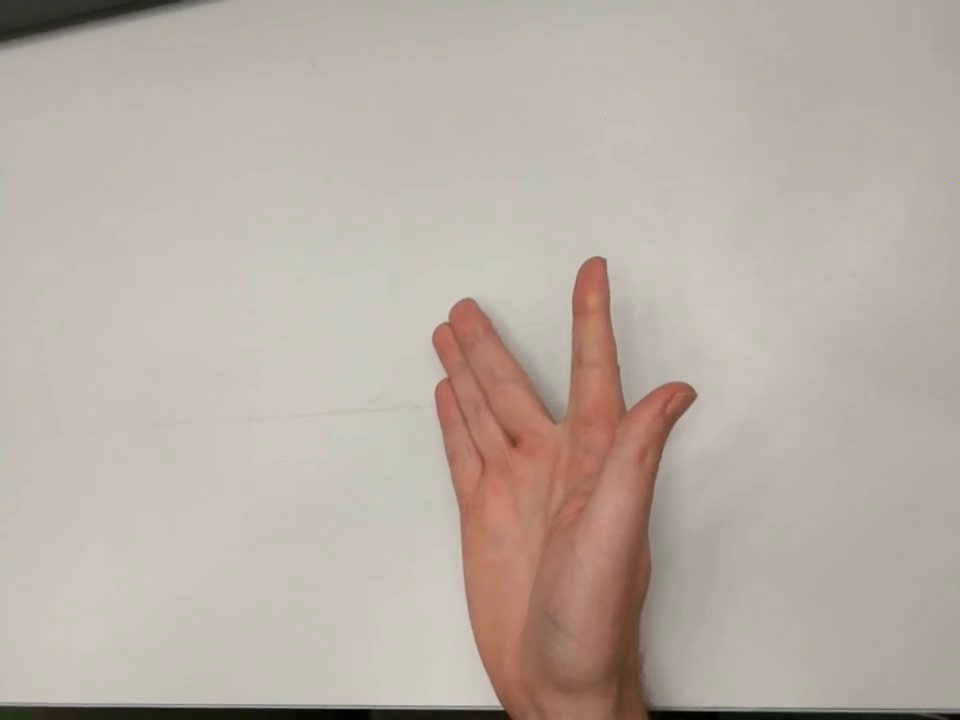
\includegraphics[width=100pt]{figures/ext_indextopair}
  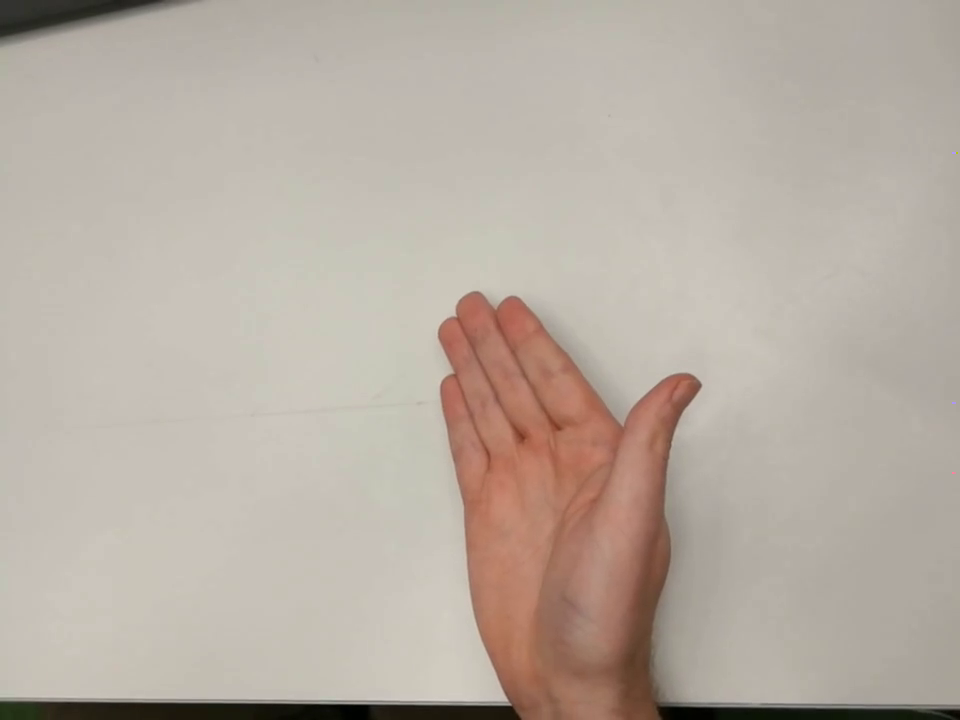
\includegraphics[width=100pt]{figures/flx_indextopair}
  \caption{G3: Moving index finger from and to pair(middle,ring,pinky)}
  \end{subfigure}
  \hspace*{\fill}
  \begin{subfigure}[t]{0.5\linewidth}
  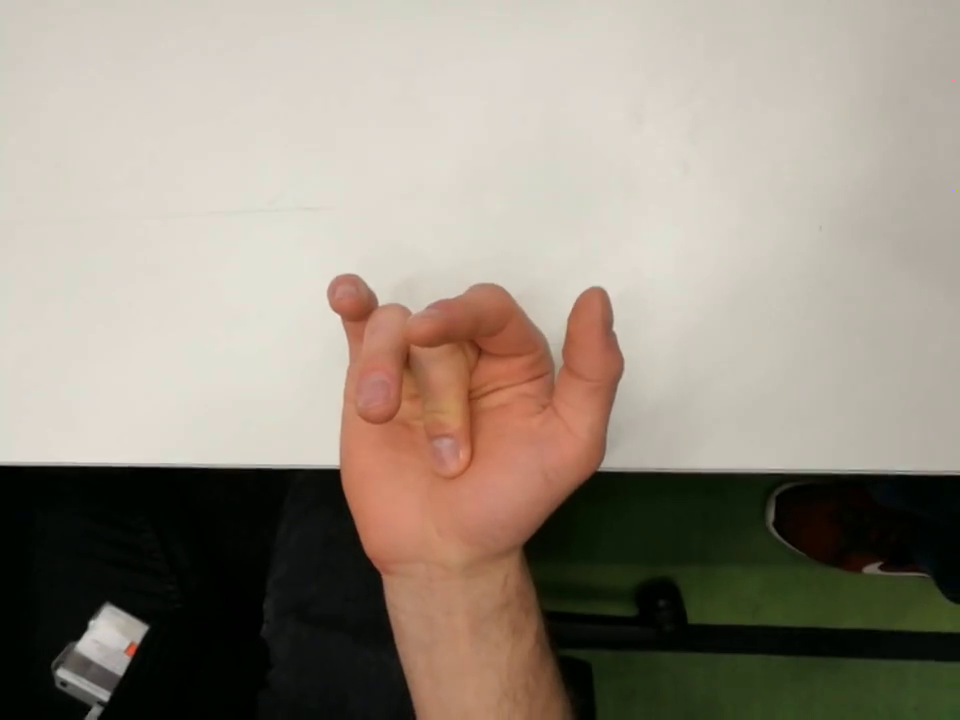
\includegraphics[width=100pt]{figures/ext_middle1}
  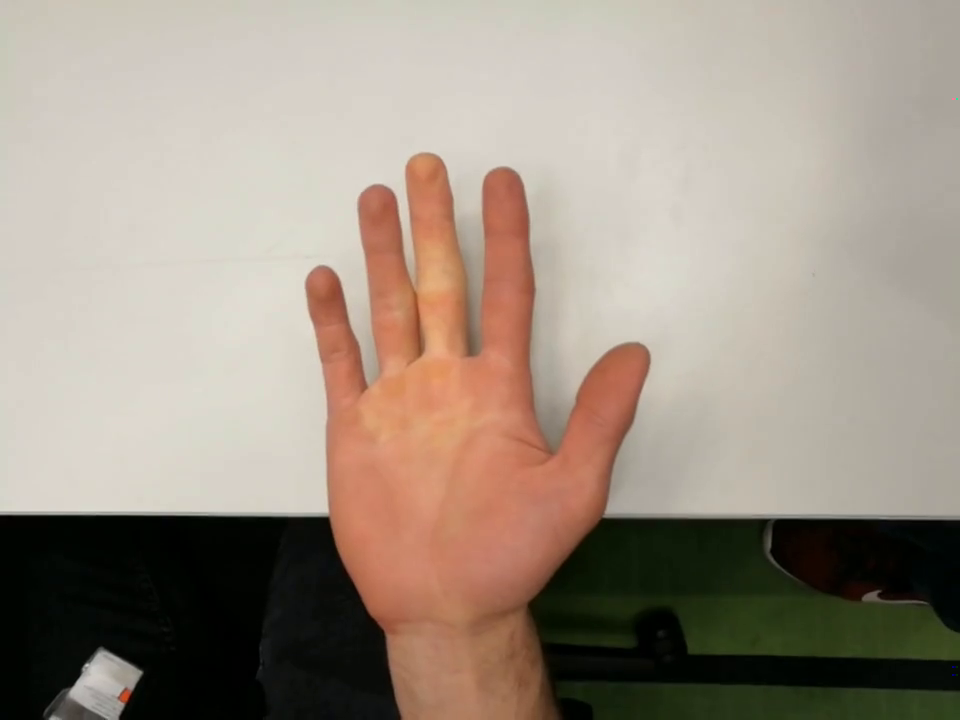
\includegraphics[width=100pt]{figures/flx_middle1}
  \caption{G4: Middle finger extension and flexion with the palm facing upwards}
  \end{subfigure}\par\medskip
  \begin{subfigure}[t]{0.5\linewidth}
  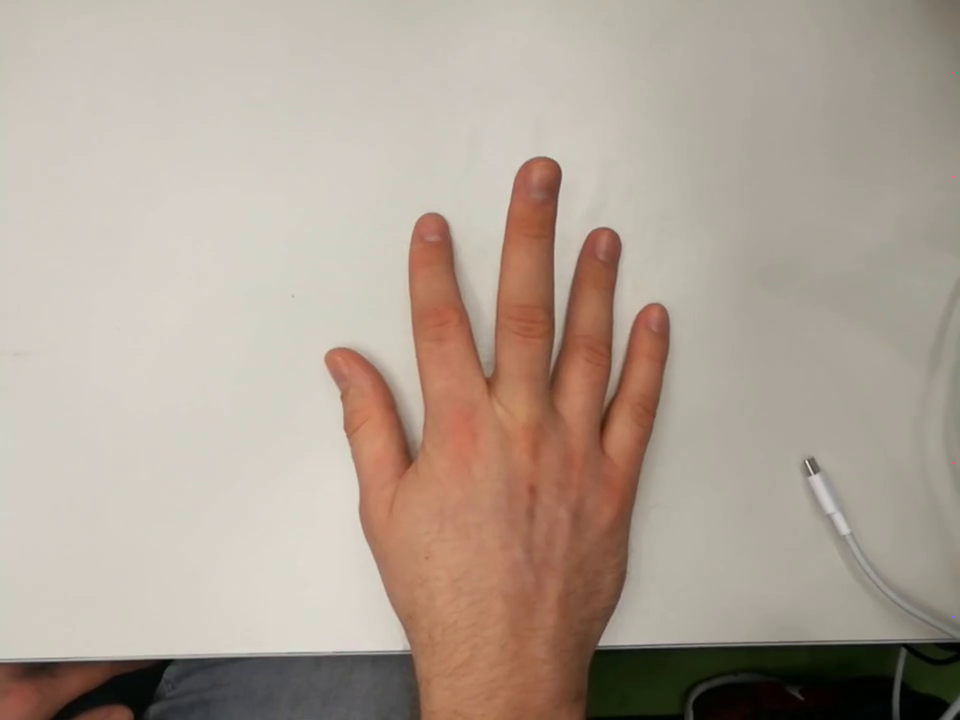
\includegraphics[width=100pt]{figures/ext_middle2}
  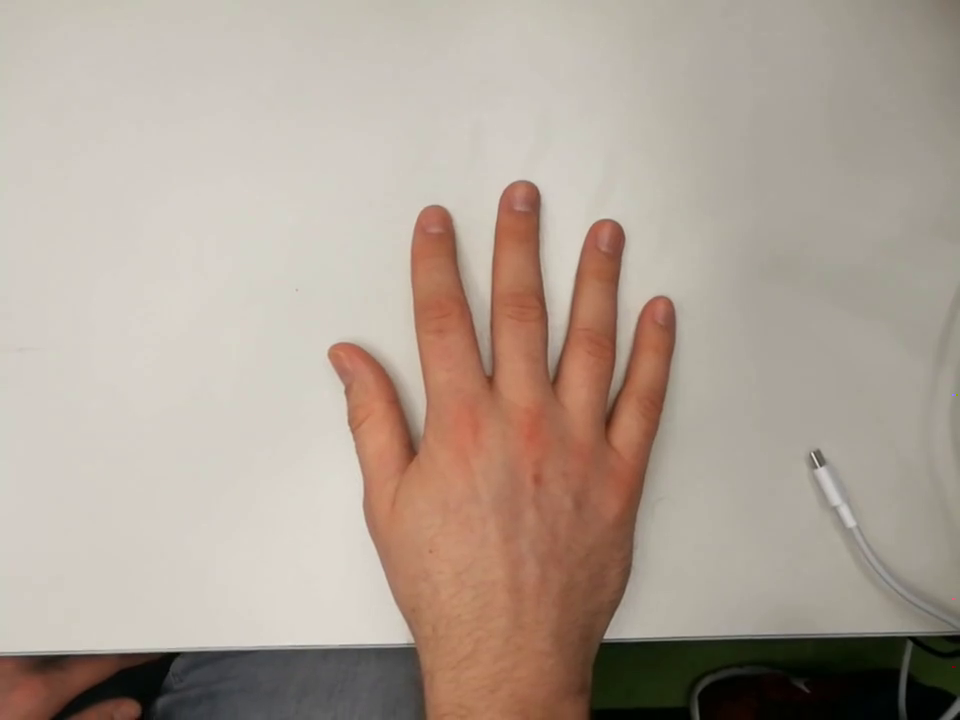
\includegraphics[width=100pt]{figures/flx_middle2}
  \caption{G5: Middle finger extension and flexion with the palm facing downwards}
  \end{subfigure}
  \hspace*{\fill}
  \begin{subfigure}[t]{0.5\linewidth}
  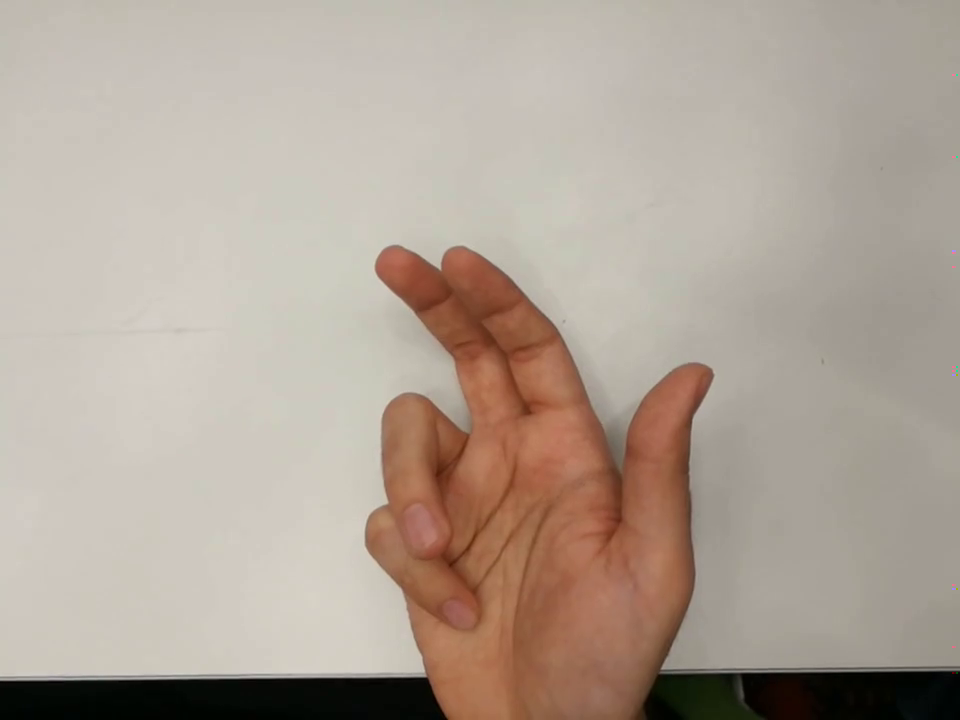
\includegraphics[width=100pt]{figures/ext_pinky1}
  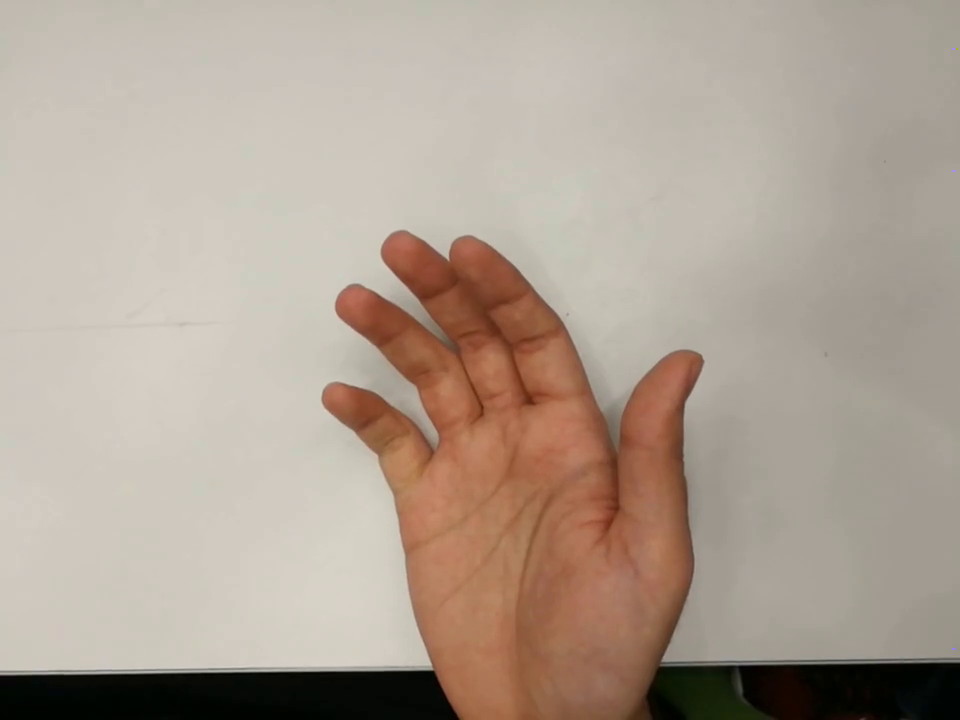
\includegraphics[width=100pt]{figures/flx_pinky1}
  \caption{G6: Pinky finger extension and flexion with the palm facing upwards}
  \end{subfigure}\par\medskip
  \begin{subfigure}[t]{0.5\linewidth}
  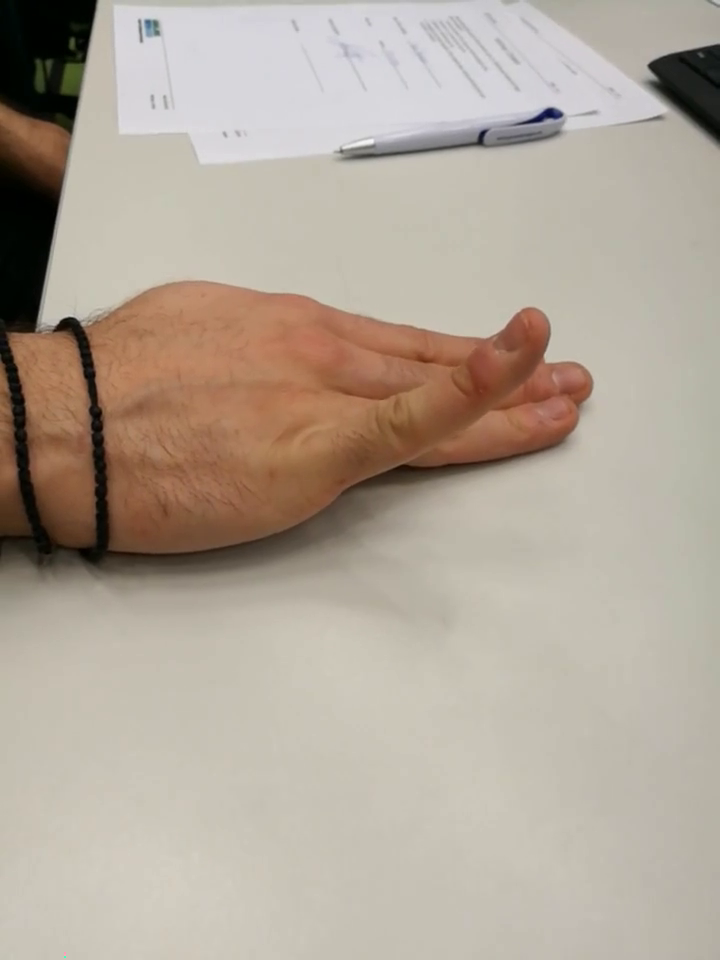
\includegraphics[width=100pt]{figures/ext_pinky2}
  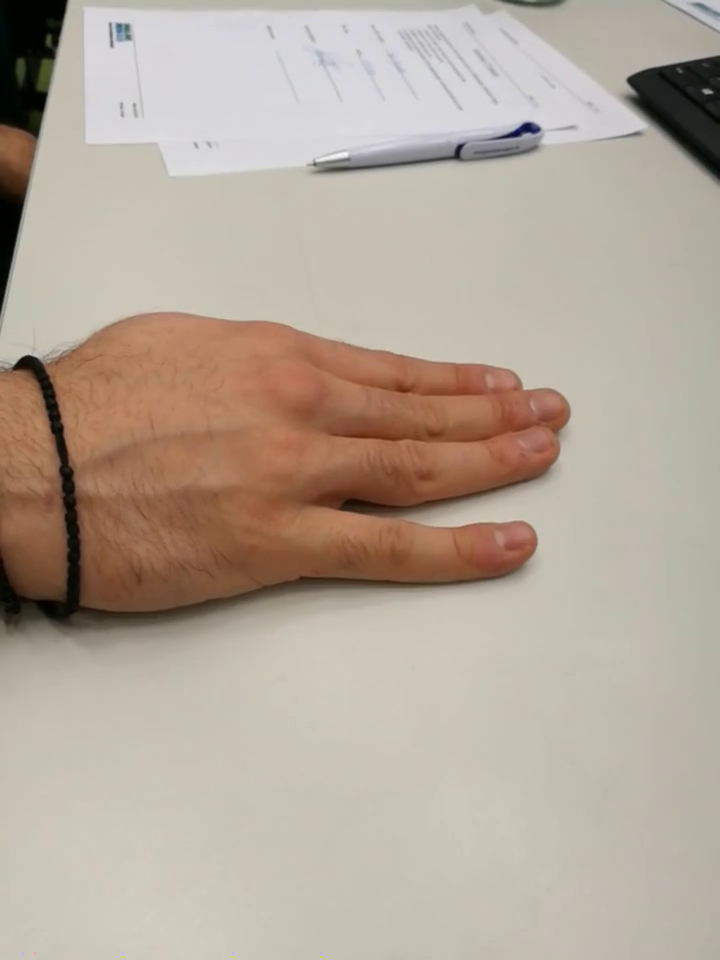
\includegraphics[width=100pt]{figures/flx_pinky2}
  \caption{G7: Pinky finger extension and flexion with the palm facing downwards}
  \end{subfigure}
  \hspace*{\fill}
  \begin{subfigure}[t]{0.5\linewidth}
  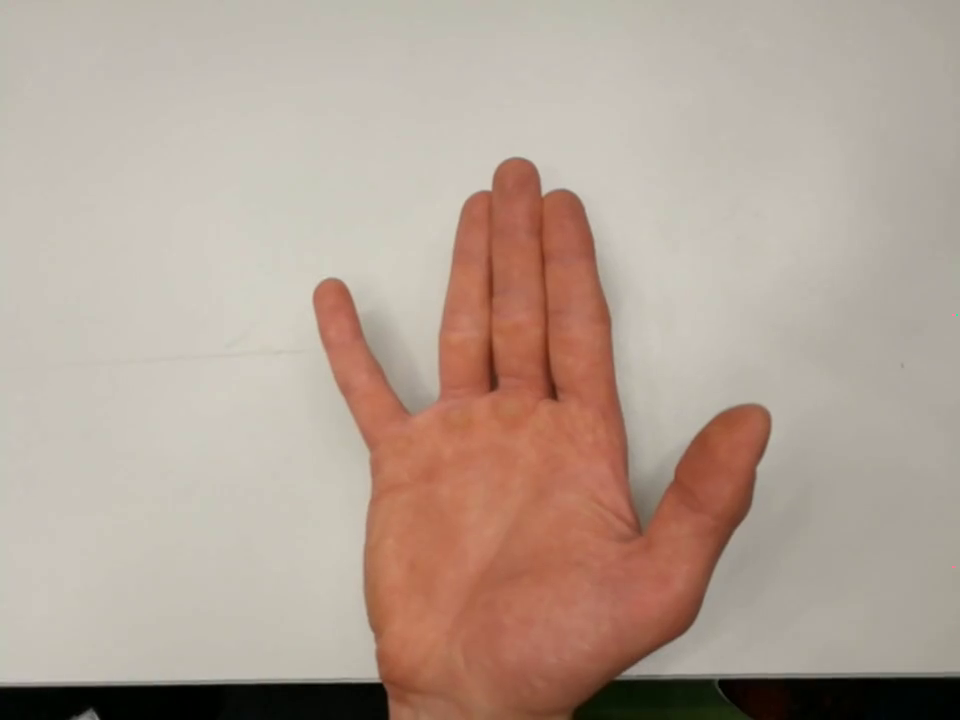
\includegraphics[width=100pt]{figures/ext_pinkytopair}
  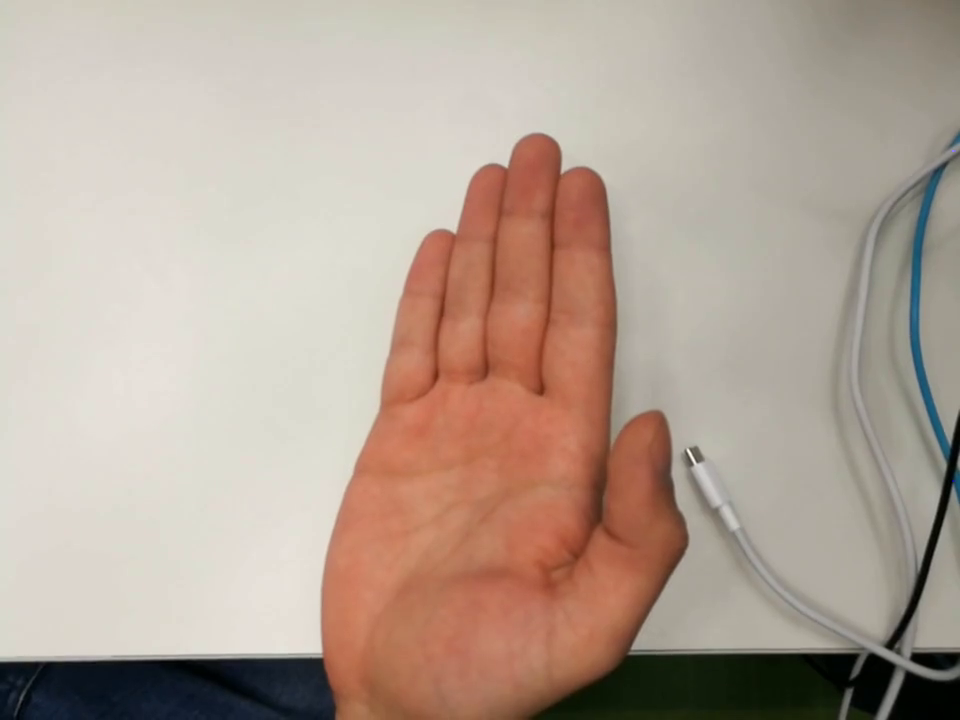
\includegraphics[width=100pt]{figures/flx_pinkytopair}
  \caption{G8: Moving pinky finger from and to pair (ring, middle, index)}
  \end{subfigure}\par\medskip
  \begin{subfigure}[t]{0.5\linewidth}
  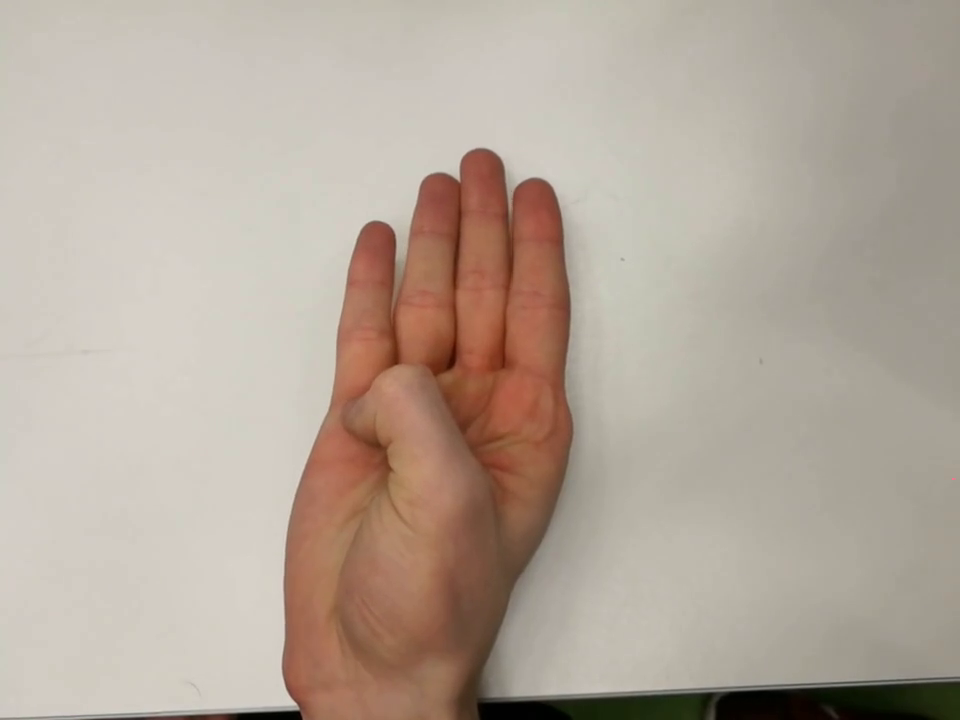
\includegraphics[width=100pt]{figures/ext_thumb1}
  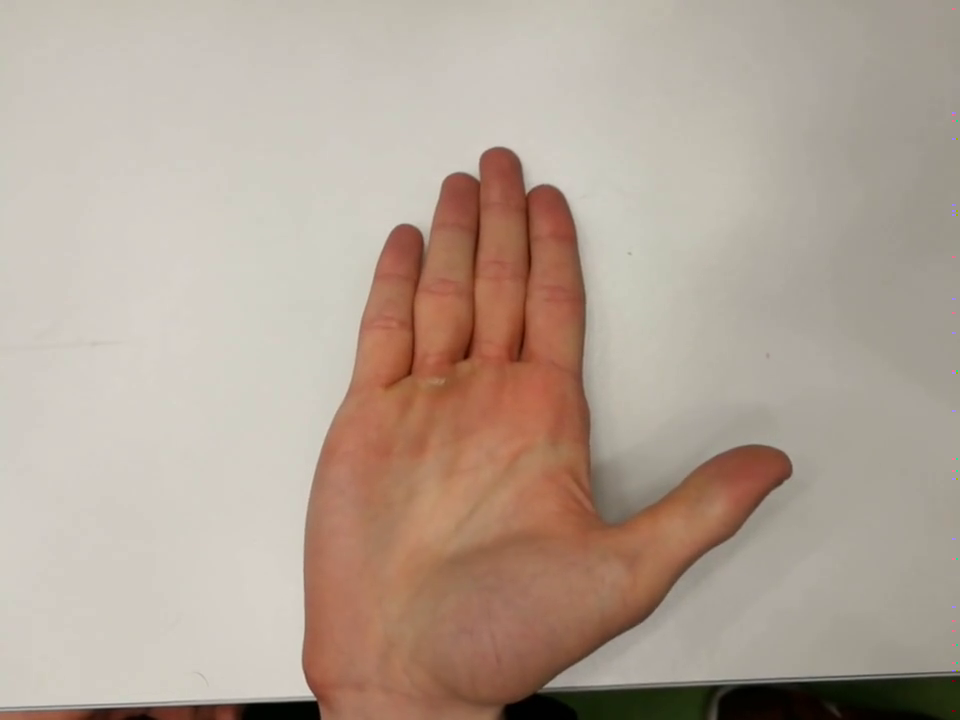
\includegraphics[width=100pt]{figures/flx_thumb1}
  \caption{G9: Thumb finger extension and flexion with the palm facing upwards}
  \end{subfigure}
  \hspace*{\fill}
  \begin{subfigure}[t]{0.5\linewidth}
  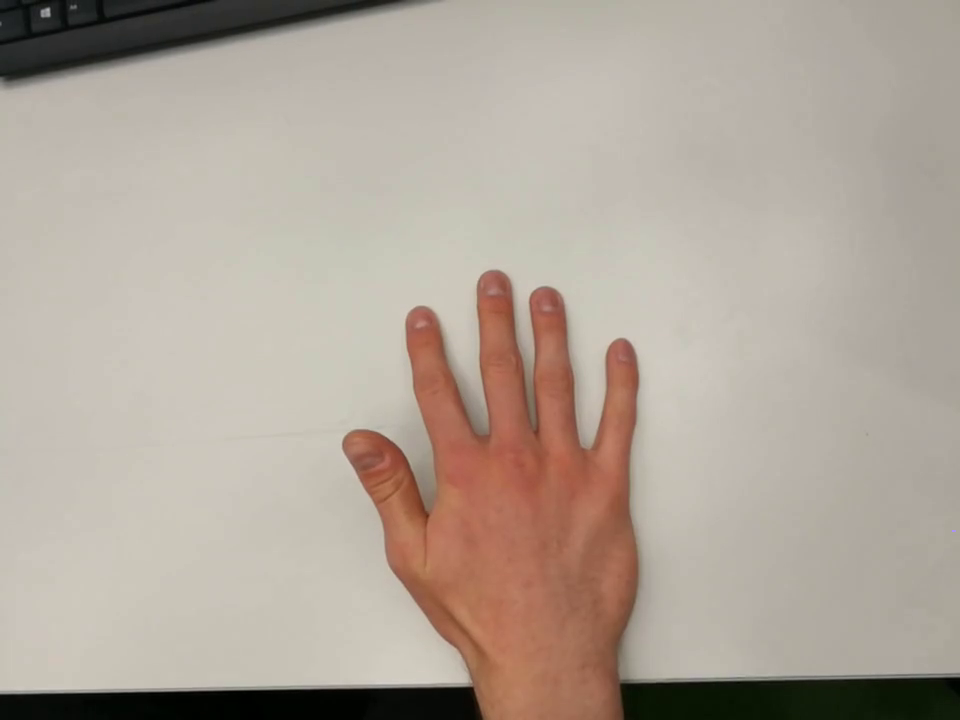
\includegraphics[width=100pt]{figures/ext_thumb2}
  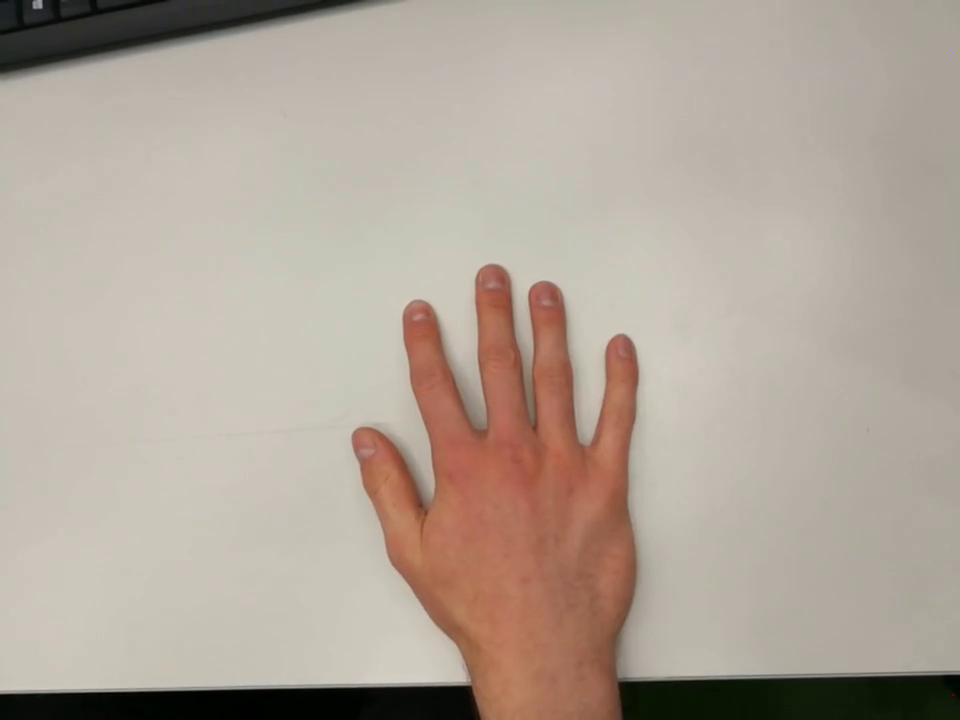
\includegraphics[width=100pt]{figures/flx_thumb2}
  \caption{G10: Thumb finger extension and flexion with the palm facing downwards}
  \end{subfigure}\par\medskip
\end{figure}
\begin{figure}
  \begin{subfigure}[t]{0.5\linewidth}
  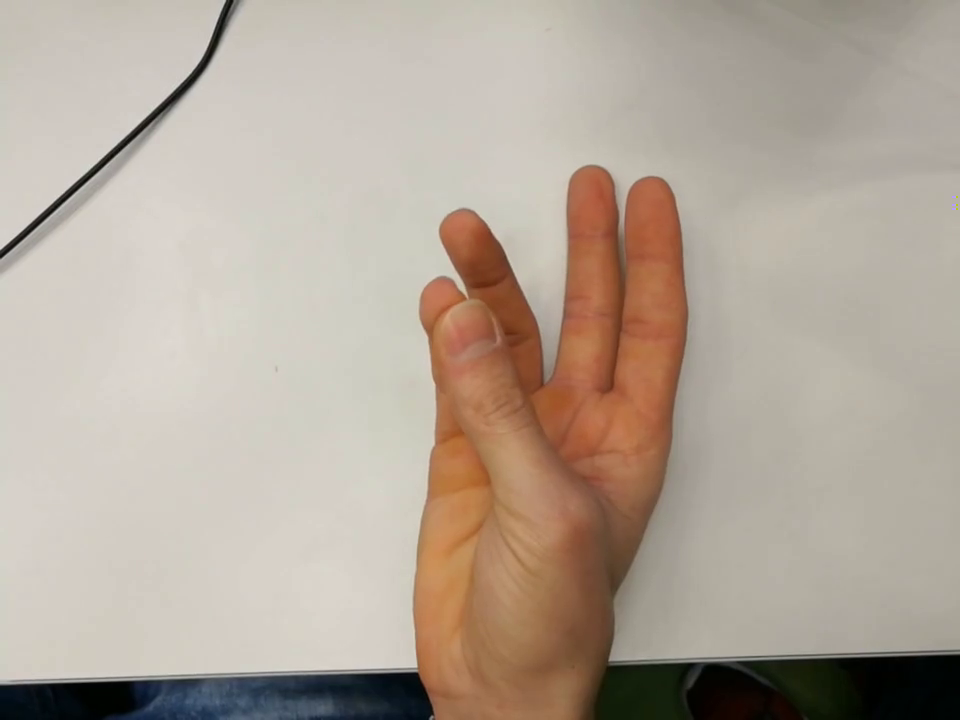
\includegraphics[width=100pt]{figures/ext_thumbtopinky}
  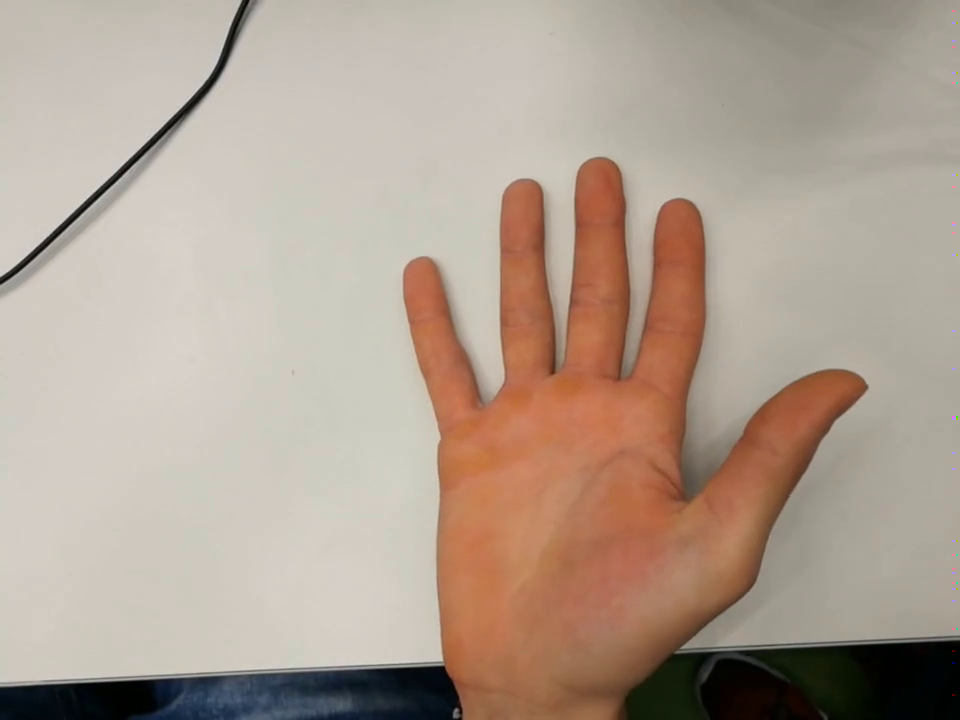
\includegraphics[width=100pt]{figures/flx_thumbtopinky}
  \caption{G11: Pairing and unpairing thumb with pinky}
  \end{subfigure}
  \hspace*{\fill}
  \begin{subfigure}[t]{0.5\linewidth}
  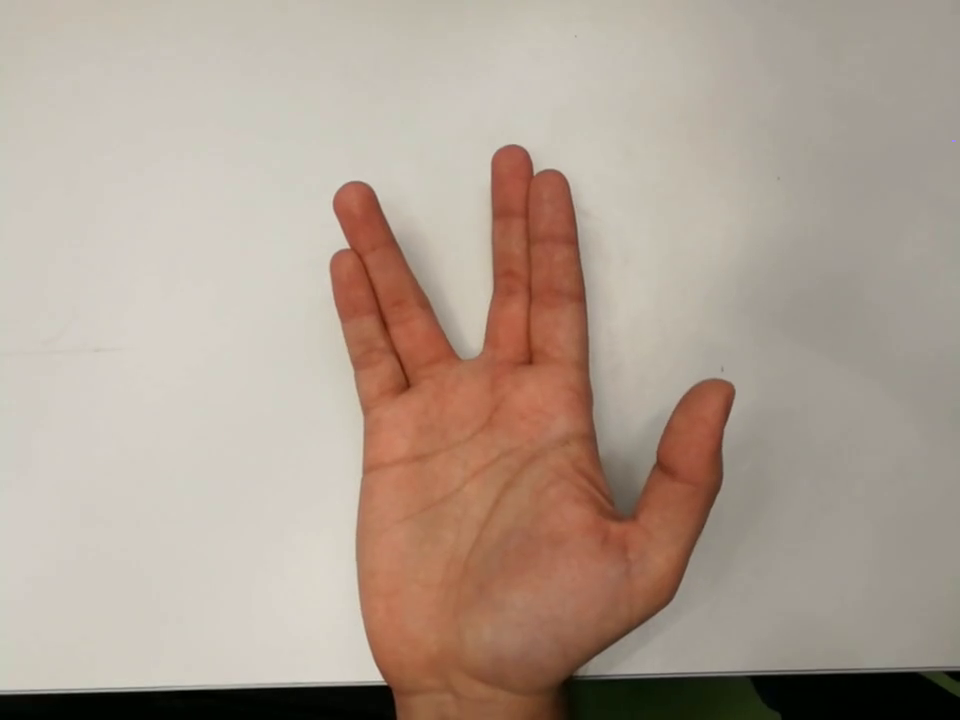
\includegraphics[width=100pt]{figures/ext_vulcan}
  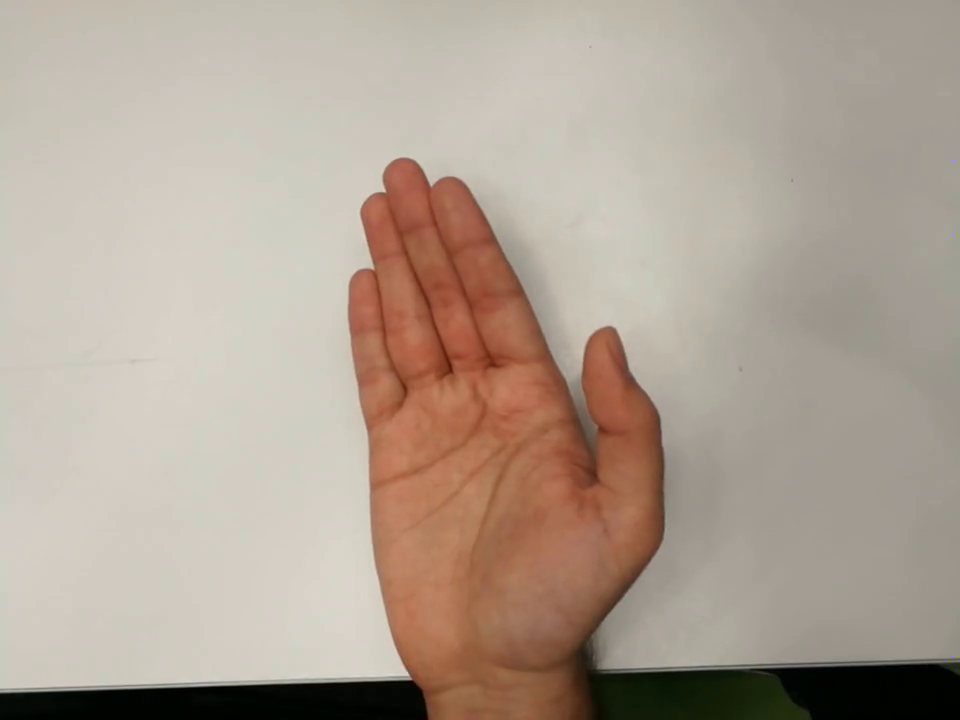
\includegraphics[width=100pt]{figures/flx_vulcan}
  \caption{G12: Pairing and unpairing pair1(index, middle) with pair2(ring, pinky)}
  \end{subfigure}\par\medskip 
  \begin{subfigure}[t]{0.5\linewidth}
  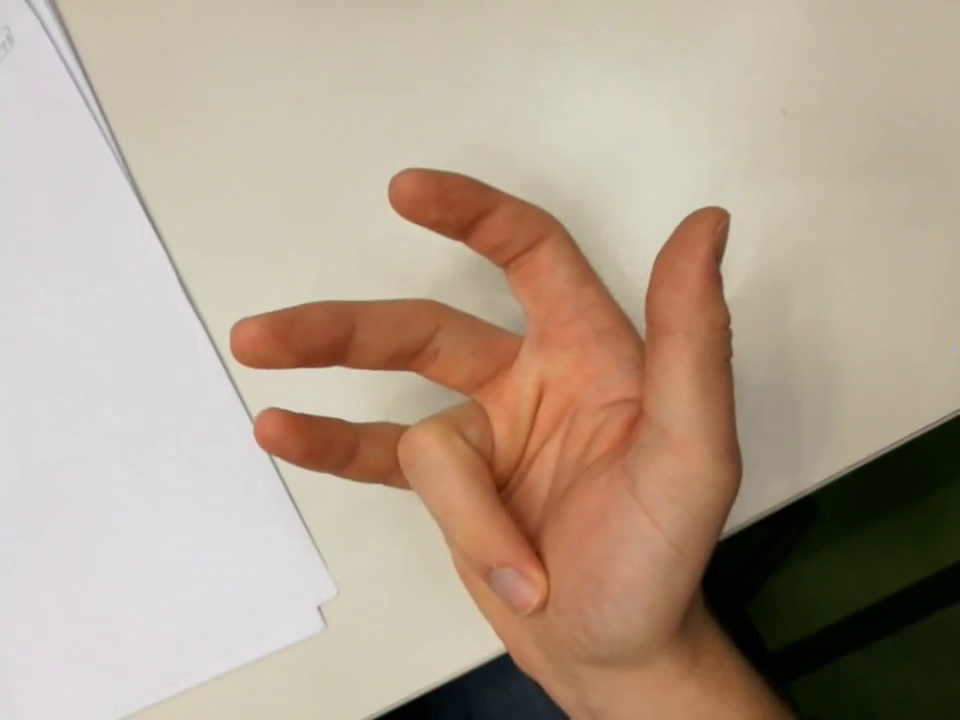
\includegraphics[width=100pt]{figures/ext_wedding1}
  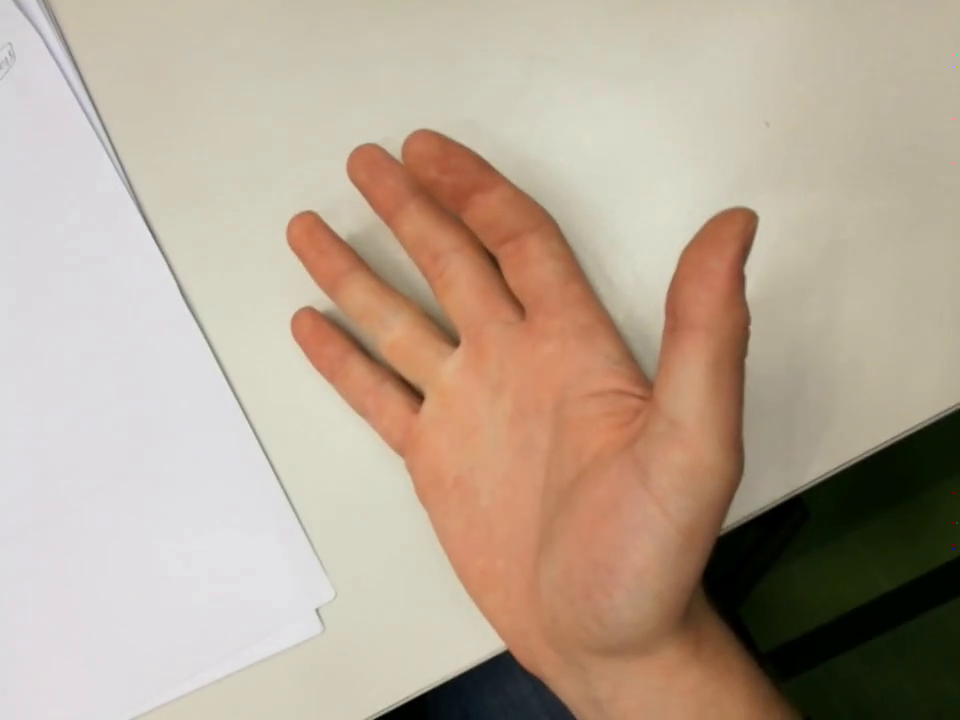
\includegraphics[width=100pt]{figures/flx_wedding1}
  \caption{G13: Rind finger extension and flexion with the palm facing upwards}
  \end{subfigure}
  \hspace*{\fill}
  \begin{subfigure}[t]{0.5\linewidth}
  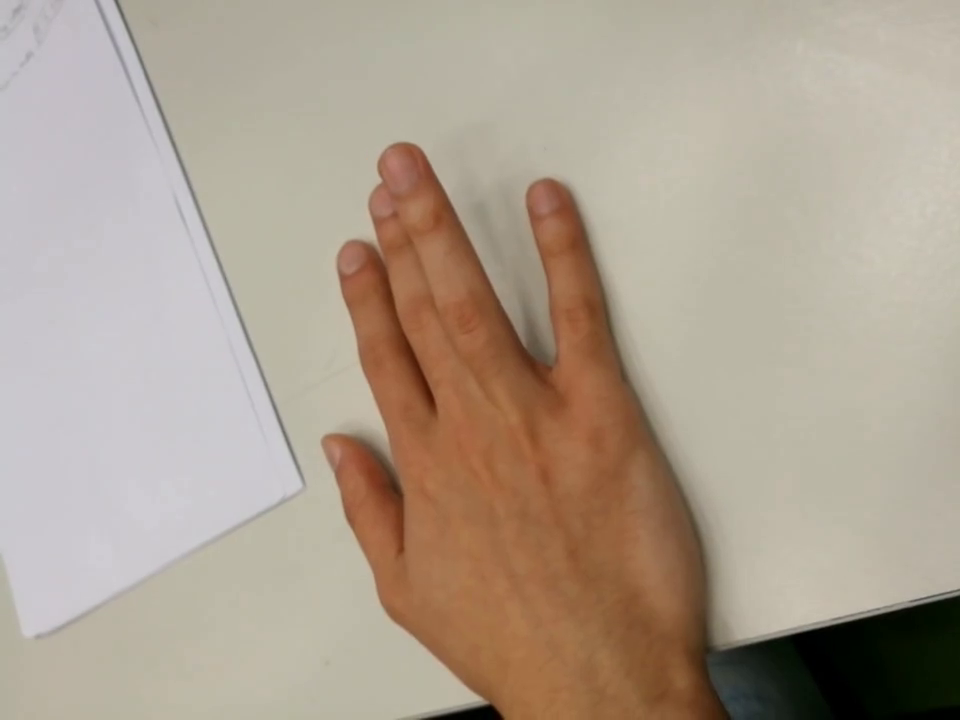
\includegraphics[width=100pt]{figures/ext_wedding2}
  \includegraphics[width=100pt]{figures/flx_wedding2}
  \caption{G14: Ring finger extension and flexion with the palm facing downwards}
  \end{subfigure}\par\medskip
\caption{14 finger gestures from 21 different subjects were acquired using the Myo armband}
\end{figure}
\chapter{Results}
In this chapter we will present the results coming from the process of parameter adjustment and the results coming from the final evaluation. During the parameter adjustment we use as an input for our neural network, EMG data with the Myo armband coming from the forearm regarding extension and flexion of the thumb. For the evaluation stage we acquired EMG signals from 21 subjects regarding extension and flexions of different gestures. 
\section{Parameter adjustment}
The first experiment we ran had the purpose to find the best average accuracies for the detection between thumb extension and flexion per feature.
\begin{figure}[h!]
\includegraphics[width=15cm,left,keepaspectratio]{figures/HL1HN5step1}
\caption{Average performances with one hidden layer, five neurons and step one}
\label{fig:HL1HN5step1}
\end{figure}
As fig. \ref{fig:HL1HN5step1} shows, we have estimated the average accuracies for the training and testing of each of the 55 folds of data we have created. The best accuracy was from the discrete wavelet bior1.3 which gave $64 \%$ detection accuracy and the worst performance was from the root-mean-square with $53.1 \%$.\\
The time for training the model and testing it for the existing amount of data has found to be prohibitively long. Therefore, due to the large quantity of data we chose for the next experiments to decrease the amount of it by increasing the step of the windowing from 1 to 64. The second experiment had the purpose to check whether the neural net with one hidden layer and five hidden nodes can give us similar or better results with less data.
\begin{figure}[h!]
\includegraphics[width=15cm,left,keepaspectratio]{figures/HL1HN5step64}
\caption{Average performances with one hidden layer, five neurons and step 64}
\label{fig:HL1HN5step64}
\end{figure}
Fig. \ref{fig:HL1HN5step64} shows slightly better results than the first batch. As we can observe in almost every feature we got better results with less data.\\
For the next experiment we decided to combine all possible combinations of the train and test data extracted  with the window step of 64 produced from the different features we selected for the current work. In total, we have 11  features and each feature has five folds for the training data and five folds for the test data. Combining all 11 features in groups of two then there are 55 combinations which is calculated by the following equation:
\begin{equation}
\binom{n}{k} = \frac{n(n-1) \cdots (n-k+1)}{k(k-1) \cdots 1} = \frac{n!}{k!(n-k)!}
\end{equation}
Taking into account that each combination is accompanied by five folds of training and test data it means that we will run $55 \times 5 = 275$ neural nets. The overall runtime of the whole experiment was $5.8$ days. The average time for one experiment was $30.7$ minutes.
In Table \ref{table:perf_features_duet} we can see the results of the average detection accuracies between extension and flexion of the thumb from testing the trained neural nets with one hidden layer and five hidden neurons. The best performances are highlighted with blue color.
\begin{table}
\renewcommand{\arraystretch}{1.2}
\begin{tabular}{ |p{1.3cm}||p{1cm}|p{1cm}|p{1cm}|p{1cm}|p{1cm}|p{1cm}|p{1.1cm}|p{1.1cm}|p{1cm}|p{1cm}|  }
 \hline
 \multicolumn{11}{|c|}{Average accuracies from the combinations of all features} \\
 \hline
 Features  & rms & stft & haar & db8 & sym4 & sym8 & bior1.3 & bior2.2 & coif3 & coif4\\
 \hline
 smooth   & $64.4\%$ &$63.0\%$ &$58.9\%$ &$65.4\%$ &$63.7\%$ &$67.1\%$ &$67.4\%$ &$65.3\%$ &$66.2\%$ &$69.3\%$ \\
 rms & - &$66.1\%$ &$61.7\%$ &$69.2\%$ &$62.9\%$ &\cellcolor{blue!35}$69.9\%$ &\cellcolor{blue!35}$70.0\%$ &$63.1\%$ &$69.0\%$ &$68.0\%$\\
 stft & - & - & $67.0\%$ &$61.6\%$ &$66.3\%$ &$60.9\%$ &$68.8\%$ &$67.9\%$ &$62.4\%$ &$63.0\%$\\
 haar & - & - & - & $67.9\%$ &$66.9\%$ &$64.0\%$ &$66.3\%$ &$62.7\%$ &$63.1\%$ &$64.8\%$\\
 db8 & - & - & - & - &$69.2\%$ &$66.7\%$ &$68.7\%$ &$59.5\%$ &$66.4\%$ &$65.8\%$\\
 sym4 & - & - & - & - & - &\cellcolor{blue!35}$70.3\%$ &$68.2\%$ &$62.0\%$ &$67.8\%$ &$66.1\%$\\
 sym8 & - & - & - & - & - & - &$66.8\%$ &$59.4\%$ &$64.2\%$ &$64.7\%$\\
 bior1.3 & - & - & - & - & - & - & - &$66.8\%$ &$69.4\%$ &$59.5\%$\\
 bior2.2 & - & - & - & - & - & - & - & - &$69.3\%$ &$65.7\%$\\
 coif3 & - & - & - & - & - & - & - & - & - &$65.9\%$\\
 \hline
\end{tabular}
\caption{Combined features and ran on neural net with one hidden layer and five hidden neurons.}
\label{table:perf_features_duet}
\end{table}
From the Table \ref{table:perf_features_duet} we can see that the best performance is when we combine the features sym4 with sym8. For the next step we decided to concatenate the sym4 with sym8 and combine their concatenation with each and every other feature from the feature set.  \\
In Table \ref{table:sym4sym8} we can see the average performances per 3 features for classification in one hidden layer and five hidden neurons network.
\begin{table}[h!]
\renewcommand{\arraystretch}{1.3}
\begin{tabular}{ |p{1.6cm}||p{1.2cm}|p{1cm}|p{1cm}|p{1cm}|p{1cm}|p{1.1cm}|p{1.1cm}|p{1cm}|p{1cm}|  }
 \hline
 \multicolumn{10}{|c|}{Average accuracies from the combinations of all features} \\
 \hline
 Features  & smooth & rms & stft & haar & db8 & bior1.3 & bior2.2 & coif3 & coif4\\
 \hline
 sym4sym8  & $58.0\%$ &$61.0\%$ &$65.1\%$ &$65.2\%$ &$64.5\%$ &$65.7\%$ &\cellcolor{blue!35}$68.7\%$ &\cellcolor{blue!35}$68.4\%$ &$67.9\%$\\
 \hline
\end{tabular}
\caption{Combined features per 3 and ran on neural net with one hidden layer and five hidden neurons.}
\label{table:sym4sym8}
\end{table}
For the next experiment we chose the second best performance from the Table \ref{table:perf_features_duet} which was between the rms and sym8. We concatenated the two features and again tested against every other feature. The Table \ref{table:rmssym8} show us the results:
\begin{table}[h!]
\renewcommand{\arraystretch}{1.3}
\begin{tabular}{ |p{1.6cm}||p{1.2cm}|p{1cm}|p{1cm}|p{1cm}|p{1cm}|p{1.1cm}|p{1.1cm}|p{1cm}|p{1cm}|  }
 \hline
 \multicolumn{10}{|c|}{Average accuracies from the combinations of all features} \\
 \hline
 Features  & smooth & stft & haar & db8 &sym4 & bior1.3 & bior2.2 & coif3 & coif4\\
 \hline
 rmssym8  & $58.1\%$ &\cellcolor{blue!35}$64.8\%$ &$59.7\%$ &$57.9\%$ &$62.1\%$ &$58.2\%$ &$62.0\%$ &$60.3\%$ &\cellcolor{blue!35}$63.3\%$\\
 \hline
\end{tabular}
\caption{Combined features per 3 and ran on neural net with one hidden layer and five hidden neurons.}
\label{table:rmssym8}
\end{table}
\newpage
For the next experiment we chose the third best performance from the Table \ref{table:perf_features_duet} which was between between the rms and bior1.3. Again, we concatenated these two features and tested against every other feature. The Table \ref{table:rmsbior13} show us the results:
\begin{table}[h!]
\renewcommand{\arraystretch}{1.3}
\begin{tabular}{ |p{1.6cm}||p{1.2cm}|p{1cm}|p{1cm}|p{1cm}|p{1cm}|p{1cm}|p{1.1cm}|p{1cm}|p{1cm}|  }
 \hline
 \multicolumn{10}{|c|}{Average accuracies from the combinations of all features} \\
 \hline
 Features  & smooth & stft & haar & db8 & sym4 & sym8 & bior2.2 & coif3 & coif4\\
 \hline
 rmsbior1.3  & $61.9\%$ &$62.3\%$ &\cellcolor{blue!35}$65.8\%$ &$62.9\%$ &$61.8\%$ &$63.3\%$ &$62.9\%$ &$62.8\%$ &\cellcolor{blue!35}$64.8\%$\\
 \hline
\end{tabular}
\caption{Combined features per 3 and ran on neural net with one hidden layer and five hidden neurons.}
\label{table:rmsbior13}
\end{table}
For the next experiment, we decided to concatenate the duplet of sym4 and sym8 and test it against all the other features and also incrementing the number of layers from one to eight layers with each consisting of 5 hidden neurons. The total number of nets that had to be trained was 585. The duration of this experiment was 73 days. The average time for each training and classification was 2.9 hours. The Table \ref{table:sym4sym8_1-5layers} shows us the results:
\begin{table}[h!]
\renewcommand{\arraystretch}{1.2}
\begin{tabular}{ |p{1.7cm}||p{1.2cm}|p{1cm}|p{1cm}|p{1cm}|p{1cm}|p{1.1cm}|p{1.1cm}|p{1cm}|p{1cm}|}
 \hline
 \multicolumn{10}{|c|}{sym4sym8} \\
 \hline
 Layers  & smooth & rms & stft & haar & db8 & bior1.3 & bior2.2 & coif3 & coif4\\
 \hline
 1 Layer  & \cellcolor{blue!35}$68.1\%$ & $61.0\%$ &$63.5\%$ &\cellcolor{blue!35}$67.0\%$ &$61.0\%$ &\cellcolor{blue!35}$68.0\%$ &$66.0\%$ &$64.4\%$ &$66.0\%$\\
 2 Layers & \cellcolor{blue!35}$69.7\%$ & $66.0\%$ &\cellcolor{blue!35}$70.5\%$ &$68.4\%$ &$69.2\%$ &$67.1\%$ &\cellcolor{blue!35}$69.5\%$ &$68.4\%$ & $67.0\%$\\
 3 Layers &\cellcolor{blue!35} $67.0\%$ & $63.7\%$ & $72.4\%$ & $70.0\%$ &$68.4\%$ &\cellcolor{blue!35}$71.2\%$ &$69.7\%$ &$69.1\%$ &\cellcolor{blue!35}$70.7\%$\\
 4 Layers & \cellcolor{blue!35}$72.0\%$ & $65.0\%$ & $71.4\%$ & $71.5\%$ &\cellcolor{blue!35}$72.1\%$ &$71.1\%$ &$70.5\%$ &$69.4\%$ &\cellcolor{blue!35}$73.0\%$\\
 5 Layers & $71.3\%$ & $67.8\%$ &\cellcolor{blue!35}$74.0\%$ &\cellcolor{blue!35}$72.5\%$ &$71.0\%$ &$71.5\%$ &\cellcolor{blue!35}$72.5\%$ &$70.5\%$ &$67.0\%$\\
 6 Layers & \cellcolor{blue!35}$74.2\%$ & $71.1\%$ & $73.0\%$ & \cellcolor{blue!35}$73.8\%$ &\cellcolor{blue!35}$74.2\%$ &$72.6\%$ &$74.1\%$ &$72.3\%$ &$71.5\%$\\
 7 Layers & $73.2\%$ & $68.6\%$ & \cellcolor{blue!35}$74.0\%$ & $73.5\%$ &$71.7\%$ &$73.0\%$ &\cellcolor{blue!35}$74.3\%$ &\cellcolor{blue!35}$73.8\%$ &$73.2\%$\\
 8 Layers &$72.9\%$ & $71.0\%$ & $72.3\%$ & $72.2\%$ &\cellcolor{blue!35}$73.5\%$ &\cellcolor{blue!35}$73.6\%$ &$73.5\%$ & \cellcolor{blue!35}$74.3\%$ &$72.0\%$\\
 9 Layers & \cellcolor{blue!35}$74.2\%$ & $63.2\%$ & \cellcolor{blue!35}$74.8\%$ & $72.8\%$ &$74.0\%$ &$73.5\%$ &$72.1\%$ & \cellcolor{blue!35}$74.4\%$ &$71.5\%$\\
 10 Layers & $73.0\%$ & $71.6\%$ & $73.8\%$ & \cellcolor{blue!35}$74.2\%$ &$72.3\%$ &$73.0\%$ &\cellcolor{blue!35}$74.1\%$ & \cellcolor{blue!35}$74.8\%$ &$73.4\%$\\
 11 Layers & \cellcolor{blue!35}$74.1\%$ & $71.8\%$ & $73.8\%$ & $74.0\%$ &\cellcolor{blue!35}$74.6\%$ &$73.7\%$ &\cellcolor{blue!35}$74.2\%$ & $73.7\%$ &$72.5\%$\\
 12 Layers & $73.3\%$ & $70.1\%$ & \cellcolor{blue!35}$74.1\%$ & $73.1\%$ & $74.3\%$ & $74.1\%$ & \cellcolor{blue!35}$74.4\%$ & $74.0\%$ & \cellcolor{blue!35}$74.8\%$\\
 13 Layers & $74.6\%$ & $70.0\%$ & $74.5\%$ & $73.7\%$ & $74.3\%$ &\cellcolor{blue!35} $74.9\%$ & \cellcolor{blue!35}$74.9\%$ & \cellcolor{blue!35}$74.8\%$ & $74.6\%$\\
 \hline
\end{tabular}
\caption{Best three performances per layer. Combined features per 3 and ran on neural net with incrementing the number of layers from one to eight.}
\label{table:sym4sym8_1-5layers}
\end{table}
Due to the time-consuming nature of the feature elimination process we decided to complete the experiments as we reached 13 layers in our neural network. Taking into account all the estimated average accuracies we plotted in 3 axes, the features according to their accuracies they had between each other in each layer.
\begin{figure}[h!]
\includegraphics[width=14cm,center,keepaspectratio]{figures/sym4sym8}
   \caption{Average performances of networks from 1 to 13 layers, five neurons each. Each network was trained with the concatenation of sym4sym8 data and tested with 9 other features. The colors represent the names of the features and are shown in the legend box.}
   \label{fig:sym4sym8} 
\end{figure}
The following plot of the heatmap of the Table \ref{table:sym4sym8_1-5layers} is helping to give us a better visualization on which features had the best improvement over the increase of the layers of the neural networks.
\begin{figure}[h!]
\includegraphics[width=17cm,center,keepaspectratio]{figures/accuracy_heatmap}
   \caption{Heatmap with the detection accuracies}
   \label{fig:accuracy_heatmap} 
\end{figure}
\section{Final evaluation}
To conduct the final evaluation we take the best parameters derived from the previous experiments for the adjustment of the parameters.\\
As we can see \ref{fig:sym4sym8} the rms feature does not perform so well as the other features. We will avoid to use 13 layers for our neural model as there is a risk of overfitting the train data. As we can notice the plateau with the best performances happen for 8 layers. Therefore, this is the number we will use for the final neural model. The features we will choose for the feature extraction are going to be db8, bior2.2, coif3, as they are the features with the best performances for 8 layers. We will evaluate the new finger gestures with a neural model which will consist of 8 layers and will train it with the triplet of sym4 and sym8 and one of the following best performed features for 8 layers: db8, bior2.2 and coif3.\\
We acquired new signals from the forearms of 21 subjects with age between 20-30. The new finger gestures we classify are the following:
The detection accuracies of the new gestures are listed below:
\begin{table}[h!]
\renewcommand{\arraystretch}{1.2}
\centering
\begin{tabular}{ |p{1.7cm}||p{1.1cm}|p{1.1cm}|p{1.1cm}|}
 \hline
 \multicolumn{4}{|c|}{sym4sym8} \\
 \hline
 Gestures  & db8 & bior2.2 & coif3 \\
 \hline
 G1 & $64.5\%$ & $74.6\%$ & $50.1\%$ \\
 G2 & $73.7\%$ & $69.6\%$ & $62.7\%$ \\
 G3 & $68.8\%$ & $68.3\%$ & $66.1\%$ \\
 G4 & $58.2\%$ & $64.4\%$ & $62.6\%$ \\
 G5 & $58.1\%$ & $51.3\%$ & $52.0\%$ \\
 G6 & $74.5\%$ & $75.2\%$ & $72.0\%$ \\
 G7 & $54.4\%$ & $53.1\%$ & $56.0\%$ \\
 G8 & $63.8\%$ & $74.2\%$ & $62.7\%$ \\
 G9 & $62.8\%$ & $57.3\%$ & $70.0\%$ \\
 G10 & $61.8\%$ & $74.7\%$ & $65.0\%$ \\
 G11 & $73.1\%$ & $68.2\%$ & $70.0\%$ \\
 G12 & $55.7\%$ & $71.2\%$ & $52.2\%$ \\
 G13 & $63.5\%$ & $73.2\%$ & $67.6\%$ \\
 G14 & $54.8\%$ & $50.8\%$ & $73.0\%$ \\
 \hline
\end{tabular}
\caption{Detection accuracies for extension and flexion of finger gestures with calibrated EMGs and trained with a neural network with 8 hidden layers and 5 hidden neurons in each layer.}
\label{table:sym4sym8_8layers}
\end{table}
The total number of neural nets that had to be trained were 42. The duration of the training all of them lasted for 5.2 days. The average time to train every neural net was 2.9 hours. 
\chapter{Discussion}
In this chapter we are going to review the steps of each stage of the pipeline we proposed and we will discuss the presented results of the parameter adjustment phase and the evaluation of the final model.
\section{Parameter Adjustment}
Although the testing of the final neural network may not give the optimal detection accuracies, the adjustment of the parameters has proven to increase the detection accuracies. Furthermore, the outputs from the ANNs varies for each initialization so a potential lower or higher detection accuracy may be a result of a random variation. During the process of adjusting the parameter we classified the data between the extension and flexion of the thumb.\\
\subsection{Increase on the window step}
Firstly, we trained a neural network with one hidden layer and five hidden neurons on each layer. The initial problem we had was that each and every clip of the isolated gestures had different durations. So, we needed to trim them into same duration clips to have a consistent size matrices because MatLab is more efficient with manipulating matrices instead of cells. Thus, on the dataset we extracted for a thumb extension and flexion we applied a window of 128 and a step of 1 between each window and this lead to constructing our same size clips. The result was to extract a lot of data which affected the training time. The training time was 12 days. The detection accuracies for the first experiment proved to be below our expectations. Firstly, to overcome the problem with the training time we decided to increase the step between the different windows. We increased the step from one to 64. When we decreased the amount of the extracted data increasing the windowing step to 64 the accuracies slightly increased as we can see in Fig. \ref{fig:HL1HN5step64}.\\
\subsection{Forward Selection, Backward Elimination: a hybrid approach}
The next combinatorial experiment was conducted to examine which features are performing well when combined in pairs. For the next block of experiments, we decided to combine every two features and then train each pair on a neural network with one hidden layer and 5 hidden neurons and test against the corresponding pair.\\
 Table. \ref{table:perf_features_duet} shows us that the best three detection accuracies were between the pair of rms-sym8 with 69.9\% accuracy, rms-bior1.3 with 70.0\% accuracy and sym4-sym8 with 70.3\% accuracy. All the data used in these experiments were extracted using the 64 window step. We can also notice in Table. \ref{table:perf_features_duet} that there is a marginal difference between the detection accuracies of the differents duplets. The lowest detection accuracy was noted for the combination of sym8 with bior2.2. However, we cannot exclude the chance of getting these detection accuracies randomly as we know that the outputs of the neural networks are fluctuating on each and every run.\\
Next, we focused on the three best performances and concatenated each pair and used it as a new, fixed pair with which we concatenate each other feature. This resulted in creating a triplet of different features concatenated together and used this triplet to train the neural network. With each different triplet we trained a neural network with one hidden layer and 5 hidden neurons and found the derived detection accuracies. We observe from the Tables. \ref{table:sym4sym8}, \ref{table:rmssym8}, \ref{table:rmsbior13} that best detection accuracies are coming from the duplet sym4-sym8. The difference between this duplet and the other two is that the duplet sym4-sym8 is consisted of wavelets with three decomposition levels.\\
For the next block of experiments we decided to take the best performed duplet which is the sym4-sym8 and combine this duplet with each other feature to train different neural networks. In this block of experiments, we incremented the number of hidden layers by one. Normally, when the detection accuracy stops improving then we stopped increasing the number of hidden layers and focused on the features that performed the best. In our case, since the  huge amount of data with the increasing number of hidden layers caused an increasing training time. Thus,  we decided to set the maximum limit for 13 layers. In the Table. \ref{table:sym4sym8_1-5layers} we see that for the triplet sym4-sym8-rms the detection accuracy follows an arbitrary pattern and noted the lowest performance as well. We note here that the features with  the best constantly increasing performance are the wavelets and in particular bior2.2 and coif3. In the following Fig. \ref{fig:accuracy_heatmap} we can see the fluctuating values between the different features for each number of layers which we used in the neural networks.
\section{Evaluation results}
According to the results we received from the classification of the evaluation data in Table. \ref{table:sym4sym8_8layers} we can not receive a confident picture of which of the features are performing well. We observe that our neural model underperformed for some gestures and performed better for some other gestures. For example, we noted the best performance for all the three features for the extension and flexion of the pinky finger. For the detection accuracy of the finger gesture G9 which is the data we acquired from the extension and flexion of the thumbs from the 21 subjects  we can conclude that there is not an overfitting. Below we will show some statistics from the performance of our neural network with the new acquired data based on the results from the Table \ref{table:sym4sym8_8layers}.\\
The average performance per feature is depicted below:
\begin{table}[H]
\renewcommand{\arraystretch}{1.2}
\centering
\begin{tabular}{ |p{3.8cm}|p{1.4cm}|p{1.4cm}|p{1.4cm}|}
 \hline
 \multicolumn{4}{|c|}{sym4sym8} \\
 \hline
  Features & db8 & bior2.2 & coif3 \\
 \hline
 Average performance & $63.4\%$ & $66.15\%$ & $63.0\%$ \\
 \hline
\end{tabular}
\caption{Average detection accuracies per feature from Table \ref{table:sym4sym8_8layers}}
\end{table}
The average detection accuracy between the different finger gestures is depicted below: 
\begin{table}[H]
\renewcommand{\arraystretch}{1.2}
\centering
\begin{tabular}{|p{1.4cm}|p{2.2cm}|p{1.4cm}|p{2.2cm}|}
 \hline
 \multicolumn{4}{|c|}{sym4sym8} \\
 \hline
  Gestures & Average performance & Gestures & Average performance \\
 \hline
 G1 & $63.0\%$ & G8  & $66.9\%$\\
 G2 & $68.6\%$ & G9  & $63.3\%$\\
 G3 & $67.3\%$ & G10 & $67.1\%$\\
 G4 & $61.7\%$ & G11 & $70.4\%$\\
 G5 & $53.8\%$ & G12 & $59.7\%$\\
 G6 & $73.9\%$ & G13 & $68.1\%$\\
 G7 & $54.5\%$ & G14 & $59.5\%$\\
 \hline
\end{tabular}
\caption{Average detection accuracies per finger gesture from Table \ref{table:sym4sym8_8layers}}
\end{table}
The variance in the results can be justified because the acquired signals are coming from 21 different subjects where the majority of them executed the protocolled finger gestures slightly differently. What's more, the height of the placement of the Myo armband on the forearm could not be in all 21 subjects exactly same but it was estimated approximately. That means that the acquired signals might be recorded from different forearm muscles from subject to subject.  Furthermore, the signals from different fingers have varying amplitude which could lead to a biased performance of the classification algorithm. Also, the fact that multiple muscles are flexing and extending the fingers can affect the results of the classification algorithm. We observed also, that  the majority of the subjects when flexing and extending their pinky finger caused the ring finger to get strained as well. Last but not least the EMG's amplitude and frequency is affected by each subject's percent of fat, muscle tissue, hairiness, muscular fatigue, the subject's age, neuromuscular diseases and the temperature of the skin. \\
A lot of literature related to our work can be found yet there are some basic differences in the tools that were used. In the work of Vijayan et al. \cite{vijayan_surface_2015}, they acquired 6-channel EMG signals from the flexion of the five fingers of the hand and for the classification they used Multi class SVMs. Their classification results for the flexions of the thumb, index, middle, ring and pinky were 100\%, 88.8\%, 94.4\%, 100\%, 83.3\% respectively. \\
In the work of Abreu et al. \cite{abreu_evaluating_2016} they acquired EMG signals with the Myo armband regarding the recognition of gestures of the LIBRAS (Brazilian Sign Language) alphabet. For the classification of the 20 different hand gestures they used SVMs. In their real time evaluation they had good performances for the letters that could be easily performed with strength and as for the gestures that could not be performed with strength or because their gestures are similar to the gestures of other letters the classifier's performance proofed to be worse.\\
In the work of Benalcázar et al. \cite{benalcazar_hand_2017} the developed an online system that could classify with 86\% detection accuracy on the contrary with 83\% detection accuracy of the Myo proprietary software on five different hand gestures such as pinch, fist, open, wave in and wave out. For the feature extraction they used rectification of the signal combined with a low-pass Butterworth filter because it reduces the noises and smooths each channel and  they classified the different hand gestures with the k-NN classification algorithm.\\
In the work of Côté-Allard et al. \cite{cote-allard_deep_2018} they recorded two datasets from the forearms of 19 and 17 able-bodied participants and they used the first dataset for the pre-training and the second dataset for the evaluation. They proposed two separate convolutional deep neural networks one for the CWT data and one for the STFT data. They concluded that the CWT-convolutional neural network outperformed the STFT-based with an average accuracy of 98.31\% for the recognition of 7 hand gestures in 17 participants.\\
In the work of Atzori et al. \cite{atzori_deep_2016} they proposed a Convolutional Neural Network for the classification of 50 hand movements acquired from 67 intact subjects and 11 transradial amputees. The whole dataset was divided into 3 subsets. The average classification accuracy of the convolutional neural network was 66.5\% on the first dataset which and 60.27\% for the second dataset. For the third dataset which consisted only from the signal of the amputees, the convolutional neural network had an accuracy of 38.09\%. To acquire the signals from the amputees they were asked to imagine imitating the movements with the missing hand as naturally as possible. 
\chapter{Conclusion}
In this thesis a classification pipeline has been developed to detect 14 different finger gestures using solely EMG signals. This chapter provides a summary of this thesis and explains the reasons behind the choices that were made. Future suggestions to improve the existed EMG method are also included in the section 5.1.\\
To build an ideal EMG based gesture recognition system should consist of an EMG signal analysis system which is precise, quick and credible. However, the purpose of this thesis is not to develop a complete functional system but rather to explore the performance of a feed forward neural network when its input is consisting of different extracted features from the EMG signals. \\ 
In this work, we proposed an EMG method for the classification of finger gestures from intact subjects. For the classification we decided to experiment with a feedforward neural network. In order to adjust correctly the parameters for our neural network we used as initial input EMG signals from my forearm for the flexion and the extension of the thumb with the palm facing upwards.\\
The motive of this work is to examine a majority of possibilities of using machine learning to classify EMG data. This work only supports the simplest neural network architecture, the fully connected feed forward neural networks. In this work we experiment with one kind of network architecture the Multi-layer Perceptron with the focus to determine which parameters are of great significance to the accuracy and possibly performance. \\
We decided to follow a hybrid approach of the forward selection, backward elimination. We started training a neural network of one hidden layer and 5 hidden neurons with all the possible duplets of the existing features. After the training, we tested also the trained neural networks and we got the detection accuracies. From the detection accuracies we got the 3 best performances. We combined each of the best three duplets with the rest features and trained another neural network with one hidden layer and five hidden neurons. The duplet with the best detection performance was chosen and we used that duplet to combine with the rest features forming triplets. With each triplet we trained feed-forward neural networks with one hidden layer and five hidden neurons but this time incrementing the number of hidden layers by one. \\
The limitation of time did not allow us to experiment with other parameters than the number of hidden layers. The maximum number of hidden layers we reached was 13. For decided for the evaluation of the data we would a number of hidden layers which would not be close to the maximum number of layers in order to avoid possible overfitting of the evaluation data. We decided to choose  8 hidden layers for the final neural network. For that decision the Fig. \ref{fig:sym4sym8} helped us to come to the conclusion that the beginning of the plateau of the accuracies started to form around for 8 hidden layers. For that specific number of hidden layers we noted which triplets gave the best detection accuracies. \\
For the evaluation stage we created a database consisting solely of EMG signals coming from 14 finger gestures of 21 intact subjects. Each finger gesture is consisting of one flexion and one extension. As aforementioned,  the final neural network had 8 hidden layers with 5 hidden neurons each. Furthermore, the final training did not happen with all the possible triplets but only for the best performed during the process of the parameter adjustment.  For each finger gesture a classifier was built in order to distinguish between the extension and the flexion and the final corresponding detection accuracy was noted. \\
Based on the results we received, we believe it is difficult to distinguish delicate finger gestures only with EMG data and that classifiers would perform poorly if we are to compare them with other vision techniques or wearable gloves. Although, the importance of the results they make us believe that EMG data could be used as an addition to systems that also depend on other types of data. One of the most significant characteristics of the Myo armband is that its EMG sensors are portable. Regarding the fact that the basis for a successful gesture recognition system are portability and convenience we believe that a hybrid approach using both visual and EMG data could be robust, compact and considerably less cumbersome than wearable gloves.
\section{Future Work}
In this section we will provide potential improvements to the current pipeline.
\subsection{Size of data}
Creating a huge dataset to include all the relevant variations helps us to resolve to a great extent the problem of considerable changes in EMG signals from person to person, as we already mentioned. This will also improve the robustness of the EMG signals regardless the potential changes of the Myo's position on the subject's arm. 
\subsection{Amount of features and reduction of the feature vector}
For this work, we used only 11 features to extract useful information. We recommend for the further exploration of the EMG signals the use of more features on them that performed well on other works similar to ours but did not apply them on this work. For example, for the further adjustment of the preprocessing phase we recommend:
\begin{itemize}
\item to experiment with the window size for the windowing part.
\item test more discrete wavelets and different decompositiong levels.
\item further experiment with the continuous wavelet transform as an alternative to DWT.
\end{itemize}
What's more, the size of the final feature vector which we used was big enough and this leads to a long run time. For the future exploration of the existing finger gesture database we recommend the application of a method which has as purpose the reduction of the dimension of the final feature vector such as the Principal Component Analysis (PCA) or Linear Discriminant  Analysis (LDA).
\subsection{Network Architectures}
This work is based on a simple feed forward network architecture. We encourage the further experimentation with other kinds of network architectures. In case we keep the time information along with the amplitude of the EMG signal we can use the Recurrent Neural Network architecture (RNN) which has the ability to remember and make use of the sequential information. This feature can be useful for analyzing a sequence of gestures.\\
Another deep learning architecture which is recently widely used achieving a considerable performance is the Convolutional Neural Network (CNN) architecture \cite{schmidhuber_deep_2015, he_deep_2016}. Even though CNN architecture is used in image analysis, it has also its applications on time-series data, such as speech recognition \cite{qian_very_2016} and gesture recognition \cite{atzori_deep_2016} . 
%%%%%%%%%%%%%%%%%%%%%%%%%%%%%%%%%%%%%%%%%%%%%%%%%%%%%%%%%%%%%
%% LITERATUR UND ANDERE VERZEICHNISSE
%%%%%%%%%%%%%%%%%%%%%%%%%%%%%%%%%%%%%%%%%%%%%%%%%%%%%%%%%%%%%
%% Ein kleiner Abstand zu den Kapiteln im Inhaltsverzeichnis (toc)
\ifnotdraft{
\addtocontents{toc}{\protect\vspace*{\baselineskip}}
\cleardoublepage
%% Literaturverzeichnis
\phantomsection % phantomsection wird benötigt, damit z.B. hyperref die richtige Seite verlinkt.
\addcontentsline{toc}{chapter}{Bibliography}
%\nocite{*} %Auch nicht-zitierte BibTeX-Einträge werden angezeigt.
\bibliography{literature/literature}%Eine Datei 'literatur.bib' wird hierfür benötigt.
\bibliographystyle{styles/vancouver}%Art der Ausgabe: plain / apalike / amsalpha / ...
}

%% Abbildungsverzeichnis
\clearpage
\addcontentsline{toc}{chapter}{List of Figures}
\listoffigures

%% Tabellenverzeichnis
\clearpage
\addcontentsline{toc}{chapter}{List of Tables}
\listoftables


%%%%%%%%%%%%%%%%%%%%%%%%%%%%%%%%%%%%%%%%%%%%%%%%%%%%%%%%%%%%%
%% ANHÄNGE
%%%%%%%%%%%%%%%%%%%%%%%%%%%%%%%%%%%%%%%%%%%%%%%%%%%%%%%%%%%%%
\appendix
\chapter{Appendix}

\section{List of Abbreviations}

\begin{acronym}[ABCDEFGH]
	\setlength{\itemsep}{-\parsep}
	
	\acro{EMG}{Electromyography}
	\acro{ANN}{Artificial Neural Network}
	\acro{CWT}{Continuous Wavelet Transform}
	\acro{DWT}{Discrete Wavelet Transform}
	\acro{IMU}{Inertia Measurement Unit}
	\acro{AI}{Artificial Intelligence}
	\acro{MLP}{Multilayer Perceptron}
	\acro{RBF}{Radial Basis Function}
	\acro{MSE}{Mean Squared Error}

\end{acronym}
% \includepdf[pages=-,offset=-2.5cm -3cm ]{figures/appendix1.pdf}


\end{document}
